%#########################################################
\chapter{Compressed Sensing Velocity Encoded Phase-Contrast Imaging}
%#########################################################
This chapter includes a brief introduction into theory of compressed sensing and provides the details of compressed sensing application to Velocity Encoded Phase-Contrast imaging (VEPC).
%=========================================================
\section{Compressed Sensing}
%=========================================================
One of the greatest challenge in MR imaging is long scan time, which is directly proportional to the number of samples collected in the Fourier domain (\textit{k-}space).
In recent years the theory of compressed sensing as well as the sampling and reconstruction framework was developed \cite{Donoho:2006cia, 2008ISPM...25...21C, Lustig:2007cua}.
%-new paragraph-%

%-new paragraph-%
Let $k(\omega)$ be the \mbox{\textit{k-}space} data collected and the inverse Fourier transform of $k(\omega)$ is a reconstructed image $a(t)$, $t = (t_1, ... t_d) \in \mathbb{Z}^d_N$
%.........................................................
\begin{equation}
	k(\omega) = \sum_t{a(t)e^{-2\pi i (\omega_1 t_1 + ... + \omega_d t_d)/N}}
\end{equation}
%.........................................................
Is it possible to recover the same image $a$ from $k(\omega)$, where $\omega = (\omega_1, ..., \omega_d) \in \Omega$ and $\#\Omega < N^d$~? The answer emerges from the fact that MR images meet two important conditions: ($i$) MR images are sparse in a certain domain and ($ii$) Fourier encoding is not coherent with these sparse transformations. 
%Therefore image can be recovered for the undersampled dataset by solving constrained optimization problem.
%~~~~~~~~~~~~~~~~~~~~~~~~~~~~~~~~~~~~~~~~~~~~~~~~~~~~~~~~~
\subsection{Data Sparsity and Undersampling}
%~~~~~~~~~~~~~~~~~~~~~~~~~~~~~~~~~~~~~~~~~~~~~~~~~~~~~~~~~
MR data in the image domain in general are not sparse, yet in another domains the sparsity can still be achieved. 
Consider the signal $\mathbf{a}(t)$ expanded in the orthonormal basis $\mathcal{W}=\left[\mathbf{w}_1 \dots \mathbf{w}_n\right]$, where $\mathbf{w_i}$ are row vectors:
%.........................................................
\begin{equation}\label{signal of interest}
\mathbf{a}(t) = \sum_{i=1}^n	x_i \mathbf{w}_i(t)
\end{equation}
%.........................................................
with $x_i$ being an inner product of $\mathbf{a}$ and $\mathbf{w}_i$. 
If signal $\mathbf{a}(t)$ is sparse it's possible to discard a certain number of coefficients in the expansion without significant loss of information. 
Thus sparsity can be quantified by the percentage of largest transformation coefficients preserved for the sufficiently good reconstruction. 
A more rigorous quantification would be to call the the signal $\mathbf{a}(t)$ $S$-sparse if it has at most $S$ nonzero elements. 
Undersampled acquisition thus will collect only a subset of $m \in M$ coefficients, where $M \subset N$:
%.........................................................
\begin{equation}
	k_j = \left< \mathbf{a}, \mathbf{s}_j \right>
\end{equation}
%.........................................................
here $\mathbf{s}_j$ is one of the $m$ rows of the sensing basis $\mathcal{S} = [\mathbf{s}_1 \dots \mathbf{s}_m]$. 
%-new paragraph-%

%-new paragraph-%
Many different sparsifying transformations can be applied, some of the most widely used are wavelet transform, discrete cosine transformation (DCT), finite difference and Gabor transform \cite{Baker:2016vs}. 
Example in Figure~\ref{WaveletCSExample} shows: magnitude MR image obtained using FGRE (Fast gradient echo) (a), its wavelet transform (b) and image obtained from top 2.5\% of the wavelet coefficients (c).
Image in Figure~\ref{WaveletCSExample}c is visually indistinguishable from image in Figure~\ref{WaveletCSExample}a thus by preserving only limited number of largest wavelet coefficients it's still possible to get a sufficiently good reconstructed image.
This approach works well when fully-sampled image is known beforehand (e.g. image compression).
In MRI experiment the image data are \textit{a priori} unknown, therefore an acquisition strategy must be adopted.
%*********************************************************
\begin{figure}[!htb]
\vspace{+0.2cm}
    \centering
    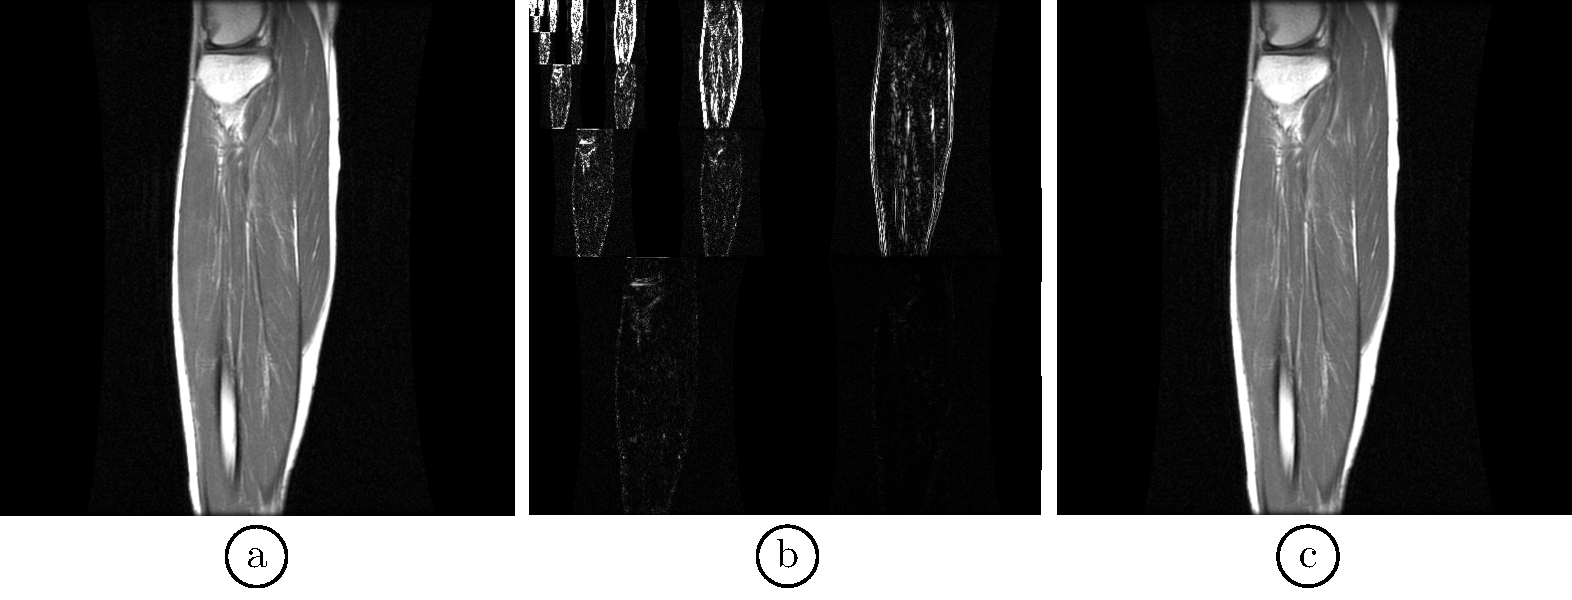
\includegraphics[width=0.9\textwidth]{Figures/CS2.pdf}
    \caption[MRI image reconstructed from top 2.5\% of its wavelet coefficients]{Magnitude FGRE image (a); wavelet transformation (b) and image reconstructed from 2.5\% of the largest wavelet coefficients (c).}
    \label{WaveletCSExample}
\end{figure}
%*********************************************************
\FloatBarrier
%~~~~~~~~~~~~~~~~~~~~~~~~~~~~~~~~~~~~~~~~~~~~~~~~~~~~~~~~~
\subsection{Incoherent Measurements and Random Sampling}
%~~~~~~~~~~~~~~~~~~~~~~~~~~~~~~~~~~~~~~~~~~~~~~~~~~~~~~~~~
Undersampled data can be represented as following:
%.........................................................
\begin{equation} \label{kspace_multicoil}
\mathbf{k} = \mathcal{A} \mathbf{x} + \sigma,
\end{equation}
%.........................................................
where $\mathcal{A} = \mathcal{S}\mathcal{W}$ is sensing matrix of size $m \times n$, $\mathbf{x}$ is a vector represented by the set of coefficients $x_i$ defined in Equation~\ref{signal of interest} and $\sigma$ is noise. 
The recovered signal $\mathbf{a}^\star$ is given by $\mathbf{a}^\star = \mathcal{W} \mathbf{x}^\star$, where  $\mathbf{x}^\star$ is the solution to the following convex minimization problem:
%.........................................................
\begin{equation} \label{COP}
\begin{aligned}
	\min_{\mathbf{z} \in \mathbb{R}^n} \quad &\norm{\mathbf{z}}_1 \\
	\text{subject to} \quad  &\norm{\mathcal{A} \mathbf{z}-\mathbf{k}}_2 < \epsilon,
\end{aligned}
\end{equation}
%.........................................................
here $\epsilon$ is a threshold parameter to control the fidelity of reconstructed data and is set to be below expected noise level $\sigma$, $\ell_1$ and $\ell_2$ -norms are defined for a vector $\mathbf{z}$ according to the Equation~\ref{L12Norm}:
%.........................................................
\begin{equation} \label{L12Norm}
\begin{aligned}
	\norm{\mathbf{z}}_1 & = \sum_{n=1}^{N}{|z_n|} \\
	\norm{\mathbf{z}}_2 & = \sqrt{\sum_{n=1}^{N}{|z_n|}^2}
\end{aligned}
\end{equation}
%.........................................................
Before discussing reconstruction procedure it's important to address the properties of the sensing matrix. 
Sensing matrix should maintain two important properties: $(i)$ incoherence and ($ii$) restricted isometry property (RIP) \cite{Candes:2005fx}.
%---------------------------------------------------------
\subsubsection{Incoherence}
%---------------------------------------------------------
For compressed sensing framework the incoherence of a sensing basis $\mathcal{S}$ and the sparsifying basis $\mathcal{W}$ is of a great importance. 
Coherence $\mu$ measures the maximum correlation between elements of $\mathcal{S}$ and $\mathcal{W}$ and is defined as:
%.........................................................
\begin{equation}
	\mu (\mathcal{S}\mathcal{W}) = \sqrt{n} \max_{1\leq p, q\leq n}{\left|\left<{s_p , w_q}\right>\right|}
\end{equation}
%.........................................................
since $\mathcal{S}$ and $\mathcal{W}$ are orthonormal lower and upper boundary for $\mu \in \left[1,\sqrt{n}\right]$. 
Suppose that $\mathbf{a}$ in basis $\mathcal{W}$ is $S$-sparse then if:
%.........................................................
 \begin{equation}
 	m\geq C \cdot \mu^2(\mathcal{S}\mathcal{W}) \cdot S \cdot \log{n}
 \end{equation}
%.........................................................
the reconstruction of the signal of interest is exact with overwhelming probability \cite{2007InvPr..23..969C}. 
Clearly this result implies that the smaller coherence leads to less number of samples required for reconstruction.
%---------------------------------------------------------
\subsubsection{Restricted isometry property}
%---------------------------------------------------------
Application of compressed sensing framework to experiment requires to consider two important issues. 
First sparsity of signal of interest is always approximate rather than exact and second is noise. 
These two issues are crucial for robustness of the reconstruction algorithm. As shown in~\cite{Candes:2006fb}, when sensing matrix $\mathcal{A}$ satisfies Restricted Isometry Property (RIP):
%.........................................................
\begin{equation}
	\left(1-\delta_S\right)\norm{\mathbf{x}}^2_2\leq\norm{\mathcal{A}\mathbf{x}}^2_2\leq\left(1+\delta_S\right)\norm{\mathbf{x}}^2_2, \quad 0 < \delta_S < 1
\end{equation}
%.........................................................
the reconstruction is accurate. In other words all subsets of S columns of sensing matrix $\mathcal{A}$ are nearly orthogonal, so $S$-sparse vectors $\mathbf{x}$ cannot be in the nullspace of $\mathcal{S}$. 
Suppose that sensing matrix $\mathcal{A}$ satisfies the RIP of order $2S$ with isometry constant $\delta_{2s} < \sqrt{2} -1$ then the solution $\mathbf{x}^\star$ of \ref{COP} obeys:
%.........................................................
\begin{equation}\label{Reconstruction error}
	\norm{\mathbf{x}-\mathbf{x}^\star}_2 \leq C_1 \frac{\norm{\mathbf{x}-\mathbf{x}_S}_1}{\sqrt{S}} + C_2 \epsilon
\end{equation}
%.........................................................
where $C_1$ and $C_2$ are constants, which are typically small, $\mathbf{x_S}$ is $\mathbf{x}$ with all $x_i$ except largest $S$ set to zero. 
Hence reconstruction error is limited by sum of noise-less term $C_1$ and term $C_2$ proportional to noise threshold parameter $\epsilon$.
Since obeying RIP guarantees robust reconstruction \cite{Candes:2006fb} it's important for sensing matrix $\mathcal{A}$ to satisfy RIP. 
It was demonstrated by Cand{\`e}~et~al.~\cite{2008ISPM...25...21C} that possible sampling schemes for sensing matrix are: sampling $m$ columns uniformly at random from $n$, i.i.d from normal distribution with mean 0 and variance $1/m$ and many other random sampling schemes satisfy RIP with high probability~if:
%.........................................................
\begin{equation}
	m\geq C \cdot S \log{\frac{n}{S}}
\end{equation}
%.........................................................
%-new paragraph-%

%-new paragraph-%
Figure~\ref{CS1} illustrates incoherence between wavelet and Fourier transformations for point spread function, here random \textit{k-}space undersampling results in incoherent interference in the wavelet domain. 
The interference spreads mostly within the wavelet coefficients of the same scale and orientation. 
%*********************************************************
\begin{figure}[!htb]
\vspace{+0.2cm}
    \centering
    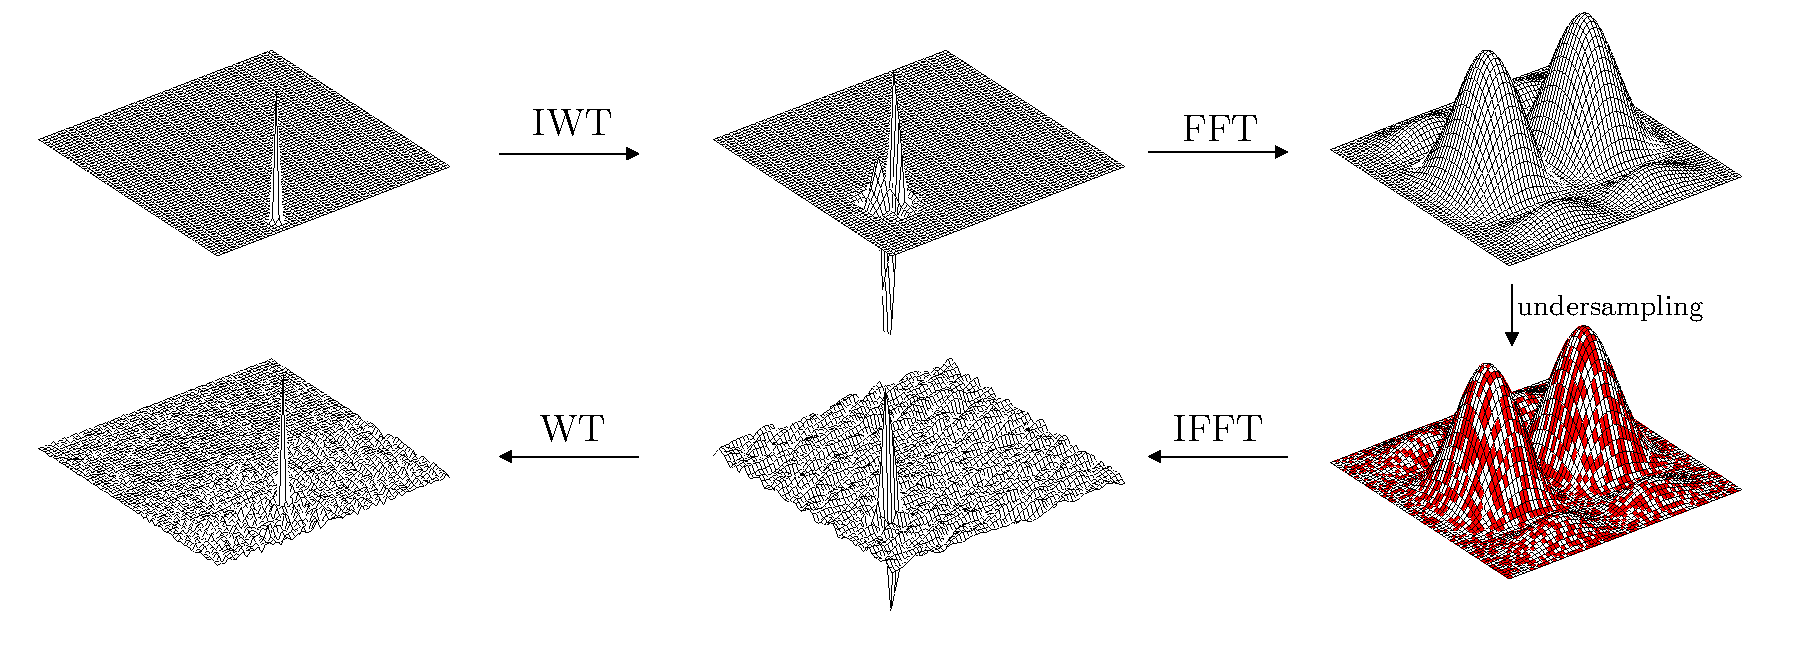
\includegraphics[width=\textwidth]{Figures/CS1.pdf}
    \caption[Incoherence between wavelet and Fourier domains]{Incoherence between wavelet and Fourier domains.}
    \label{CS1}
\end{figure}
%*********************************************************
%~~~~~~~~~~~~~~~~~~~~~~~~~~~~~~~~~~~~~~~~~~~~~~~~~~~~~~~~~
\subsection{Solution to the Constrained Optimization Problem}
%~~~~~~~~~~~~~~~~~~~~~~~~~~~~~~~~~~~~~~~~~~~~~~~~~~~~~~~~~
Reconstruction process requires to solve the constrained optimization problem~(Equation~\ref{COP}). 
For the velocity encoded MR signal this problem can be restated as following:
%.........................................................
\begin{equation} \label{CS COP}
\begin{aligned}
	\min_{\mathbf{I}}  \quad &\norm{\mathcal{F}_t \, \mathbf{I}}_1 \\
	\text{subject to} \quad  &\norm{\mathcal{F}_s \, \mathbf{I}-\mathbf{k}}_2 < \epsilon,
\end{aligned}
\end{equation}
%.........................................................
where vector $\mathbf{I}$ is an image of interest, sparsifying transform $\mathcal{F}_t$ is temporal Fourier operator, $\mathcal{F}_s$ is spatial Fourier operator, and vector $\mathbf{k}$ is undersampled MR \mbox{\textit{k-}space} data. 
Development of efficient solution algorithms to problem stated in Equation~\ref{CS COP} has been a subject of the research for many years by now. 
Multiple computational approaches exist and some of the most known and widely used are: Convex Relaxation, Iterative Thresholding, Gradient Pursuit and other~\cite{Qaisar:2013ff}. Nonlinear conjugate gradient method is one of the possible choices.
%---------------------------------------------------------
\subsubsection{Nonlinear conjugate gradient method}
%---------------------------------------------------------
Due to presence of noise in vector $\mathbf{k}$ constrained optimization problem~\ref{CS COP} should be relaxed to the least squares problem \cite{Yin:2011ts}:
%.........................................................
\begin{equation} \label{CS UOP}
	\min_{\mathbf{I}} \quad \norm{\mathcal{F}_s \mathbf{I} - \mathbf{k}}_{2}^{2} + \lambda_1 \, {\norm{\mathcal{F}_t \mathbf{I}}}_1
\end{equation}
%.........................................................
where $\lambda_1$ is the Lagrangian multiplier of the constraint from the Equation~\ref{CS COP}, which controls the tradeoff between sparsity term ($\ell_1$-norm term) and image consistency ($\ell_2$-norm term). 
Nonlinear conjugate gradient method (NCG) allows to solve minimization problem (Equation~\ref{CS UOP}) numerically if gradient  of the cost function $f(\mathbf{I})$ defined by Equation~\ref{CS UOP} can be computed \cite{Lustig:2007cua}. 
The second term of the cost function is an $\ell_1$-norm defined as a sum of absolute values, its derivative is not defined at $I_i = 0$, therefore an approximation by a smooth function is necessary. 
The most computationally efficient choice is $\left| x \right| \approx \sqrt{x^2 + \mu}$ \cite{Ramirez:2014up}. 
The gradient of $f(\mathbf{I})$ is then approximated:
%.........................................................
\begin{equation}
	\nabla f(\mathbf{I}) =  2 \mathcal{F}_s^* \left(\mathcal{F}_s \, \mathbf{I}-\mathbf{k} \right) + \lambda \mathcal{F}_t^*\mathcal{U}^{-1}\mathcal{F}_t\mathbf{I}
\end{equation} where $\mathcal{U}$ is a diagonal matrix defined as following:
\begin{equation}
	\mathcal{U}=\DiagMat{\sqrt{(\mathcal{F}_t\mathbf{I})^*_i \, (\mathcal{F}_t\mathbf{I})_i + \mu }}
\end{equation}
%.........................................................
with smoothing parameter $\mu \in \left[ 10^{-15} , 10^{-6} \right]$ \cite{Lustig:2007cua}.
NCG method is summarized in the following outline:
%-new paragraph-%

%-new paragraph-%
\noindent \begin{samepage} \textbf{NCG outline} \\
%+++++++++++++++++++++++++++++++++++++++++++++++++++++++++++++++++++++++++++++++++++++++++++++++++++++++
\indent \qquad \qquad \textit{input:} \, $f(\mathbf{I})$ - cost function, $\alpha$, $\beta$ - line search parameters\\ 
\indent \qquad \qquad \textit{output:} $\mathbf{I}$ - reconstructed image\\
\noindent\rule{15cm}{0.4pt} \\
$n=0$ \quad $I_0 = 0$ 
\begin{itemize}
	%\renewcommand{\labelitemi}{\scriptsize$-$}
	\item Initial search direction: $g_0 = \nabla f(I_0)$; $\Delta I_0 = -g_0$
	\item Backtracking-Armijo line search: $\tau = 1$
		\begin{itemize}
			\item \textbf{while} \quad $f(I_0 + \tau \Delta I_0) \leq f(I_0) + \alpha \tau \cdot \Re(g^*_0 \Delta I_0)$ \, \textbf{do} \, $\tau = \beta \tau$ \quad ($\star$)
		\end{itemize}
	\item Update search direction:
		\begin{itemize}
			\item $I_1 = I_0 + \tau \Delta I_0$, $g_1 = \nabla f(I_1)$, $\gamma = \cfrac{\norm{g_1}^2_2}{\norm{g_0}^2_2}$
			\item $\Delta I_1 = -g_1 + \gamma \Delta I_0$
		\end{itemize}
	\item $n=1$ 
\end{itemize} \vspace{-3mm} \noindent\rule{15cm}{0.4pt} \\
%+++++++++++++++++++++++++++++++++++++++++++++++++++++++++++++++++++++++++++++++++++++++++++++++++++++++
\textbf{for} \quad $0<n<N$, where $n \in \mathbb{N}$, $N$ - maximum number of iterations \quad \textbf{do}
\begin{itemize}
	%\renewcommand{\labelitemi}{\scriptsize$-$}
	\item Backtracking-Armijo line search: 	$\tau = 1$
		\begin{itemize}
			\item \textbf{while} \quad $f(I_{n} + \tau \Delta I_{n}) \leq f(I_{n}) + \alpha \tau \cdot \Re(g^*_{n} \Delta I_{n})$  \, \textbf{do} \, $\tau = \beta \tau$ \quad ($\star\star$)
		\end{itemize}
	\item Update search direction:
		\begin{itemize}
			\item $I_n = I_{n-1} + \tau \Delta I_{n-1}$, $g_n = \nabla f(I_n)$, $\gamma = \cfrac{\norm{g_n}^2_2}{\norm{g_{n-1}}^2_2}$
			\item $\Delta I_n = -g_n + \gamma \Delta I_{n-1}$
		\end{itemize}
	\item $n=n+1$ 
\end{itemize}
\textbf{end} \\
\noindent\rule{15cm}{0.4pt}
\end{samepage}\\
\newpage

%+++++++++++++++++++++++++++++++++++++++++++++++++++++++++++++++++++++++++++++++++++++++++++++++++++++++
At each iteration Backtracking-Armijo line-search is used since general backtracking line search fails to prevent the step $\tau$ from getting too large relative to the decrease~in~$f$. 
The Armijo-Goldstein condition ($\star$  and $\star \star$ in NCG outline) has a second term on the right-hand side requiring the achieved reduction in $f$ to be at least a fixed fraction $\alpha$ of the reduction promised by the first term of the Taylor series of $f(I_n)$~\cite{Armijo:1966di}. 
Both parameters $\alpha$ and $\beta \in (0,1)$. 
Compared to conjugate gradient (CG) method where $f$ is quadratic NCG has a number of choices for $\gamma$ parameter~\cite{Hager:2006wp}. 
Two most popular  are Fletcher-Reevs (given above in the NCG outline) and Polak-Ribi\`ere. 
The Fletcher-Reeves method converges if the starting point is sufficiently close to the desired minimum, whereas the Polak-Ribi\`ere method can, in rare cases, cycle infinitely without converging~\cite{Shewchuk:1994uc}.
%=========================================================
\section{Application of Compressed Sensing Methods for Monitoring Skeletal Muscle Kinematics}
\label{sec: CS_paper}
%=========================================================
Magnetic Resonance imaging has been established as a viable technique to study muscle kinematics (including strain mapping)~\cite{RNS31, RNSS4, RNCS3, RNCS4, RNCS5}. 
Several studies have established the feasibility of the VEPC based MRI technique for monitoring muscle velocity and strain rate mapping during passive muscle motion and for different contraction modes (e.g., for isometric, concentric and eccentric contraction patterns)~\cite{RNCS3, RNCS4, RNCS5} as well applied it to study differences in aging and young muscle as well as pre- and post- unloading~\cite{RNS16, Malis:2018fr}. 
However, the limitation of the VEPC is the long scan time that requires execution of $\sim 75$ consistent contractions for dynamic imaging ($\sim \SI{2}{\minute}~\SI{40}{\second}$).
Several methods have been developed to maintain the consistency of contraction; e.g., by providing a visual feedback of the measured force superposed on the target force curve~\cite{RNS16, Malis:2018fr}. 
However, this still limits the force that can be maintained for the duration of the scan; this is usually set at 30-35\% Maximum Voluntary Isometric Contraction (MVIC) to enable $\sim 75$ consistent contractions. 
Studying muscle kinematics for several \%MVICs including higher \%MVICs may provide better insights into differences in muscle kinematics between normal and diseased (e.g., sarcopenia, disuse atrophy, dystrophy) conditions~\cite{RNS16, Malis:2018fr}. 
The long scan times also prevent acquisition of multiple slices to extract the full 3D strain or strain rate tensor. 
Further, in order to decrease scan times, views per segment (VPS) up to 4 are employed, but this limits the acquired temporal resolution of the scans. 
A faster VEPC sequence with improved temporal resolution could possibly expand the domain of exploration of muscle kinematics. 
%-new paragraph-%

%-new paragraph-%
Compressed sensing (CS) has been applied successfully and extensively in MRI to accelerate scan times~\cite{Lustig:2007cua}. 
CS allows for reconstruction of undersampled MRI data based on the concept that an image with a sparse representation in a known transform domain can be recovered (without artifacts) from randomly undersampled \mbox{\textit{k-}space} data using a non-linear reconstruction. 
The maximum acceleration (CS undersampling factor) will be determined by the image sparsity in the transform domain; the experimental observation is that the number of required samples is approximately $\sim 4$ times the number of non-zero coefficients in the transform domain. 
Various sparsifying transforms have been introduced such as wavelet, Principal Component Analysis (PCA) and Fourier Transform (FT)~\cite{Lustig:2007cua}. 
For 2D imaging, practical considerations limit the randomness to the phase encode direction ($k_y$) while for 3D acquisitions, random undersampling can be performed in the two phase-encode directions ($k_y$ and $k_z$) allowing for higher acceleration factors. 
Further, in 2D dynamic imaging as in 2D VEPC, researchers have exploited the fact that each temporal frame can have a different random phase encode pattern and a joint reconstruction of all temporal frames exploits the randomness in two axes ($k_y$\textit{-t}) allowing for higher acceleration factors compared to independent reconstructions of each temporal frame. 
$k_y$\textit{-t} CS reconstruction has also been integrated with multiple coil sensitivity profiles to perform a joint reconstruction of raw data from all the coils: this allows higher acceleration factors than CS without multiple coils that still yields images without significant artifacts. 
This latter technique, termed $k_y$\textit{-t} SPARSE SENSE to reflect the combination of multi-coil (parallel) imaging and CS techniques, has been applied to first-pass cardiac perfusion imaging as well as to studying cardiovascular and hepatoportal vascular dynamics~\cite{RNCS9, RNCS10}. 
However, the $k_y$\textit{-t} SPARSE SENSE technique has not been applied to imaging muscle kinematics. 
It should be noted that muscle velocities are much lower than that encountered in cardiac or portal and hepatic veins blood flow imaging ($venc = \SI{80}{\centi\meter/\second}$), so the velocity encoding gradients are much larger for the VEPC sequence to map muscle motion ($venc = \SI{10}{\centi\meter/\second}$). 
The larger velocity encoding gradients result in noisier images, so that integrating compressed sensing with VEPC sequences mapping lower velocities may pose additional challenges. 
One recent paper reported 4D VEPC integrated with compressed sensing applied to muscle dynamics~\cite{RNCS11}.
The latter paper performed 3D volume acquisition with undersampling in the $k_y$ and $k_z$ axes with 3-directional velocity encoding. 
In order to leverage the undersampling in the slice direction, a fairly high number of partitions is required (e.g. $\Rightarrow 32$) that results, for the best acceleration factor reported in the latter paper ($\sim \times 6.4$), in scan times of $\sim \SI{2}{\minute}~\SI{46}{\second}$. 
Admittedly, the optimum approach for 3D strain rate tensor computation is to acquire in 3D with 3 directional velocity encoding to cover the entire muscle. 
However, the long acquisition time of the 3D sequence even with ($\sim \times 6.4$) undersampling~\cite{RNCS11} limits its application with regards to the goal of the current work to reduce the acquisitions to less than a minute. 
Further, earlier experimental observation was~\cite{Malis:2018fr}, that with appropriate orientation of the acquisition slice in the plane of the muscle fibers (e.g., oblique sagittal for the medial gastrocnemius), 5 contiguous slices of $\SI{5}{\milli\meter}$ thickness allows the extraction of the 3D strain/strain rate (SR) tensor in 3 slices and this is sufficient to capture the spatial variation of the 3D strain tensor along the length of the muscle. 
%-new paragraph-%

%-new paragraph-%
The advantages of a faster VEPC sequence for muscle imaging is that it will allow scans to be completed with a shorter number of contraction cycles; this will expand the applicability to cohorts that are limited in their ability to sustain consistent contraction levels for a large number of repetitions. 
These cohorts include older subjects (normal and sarcopenic) and subjects with skeletal muscle disorders such as disuse atrophy dystrophy. 
Further, a short VEPC sequence will also enable acquisitions at higher \%MVIC (and at several \%MVIC) in contrast to current MRI based muscle kinematics studies limited to a single \%MVIC ($\sim 35$\%MVIC) achievable using traditional longer VEPC sequences~\cite{RNS16, Malis:2018fr}. 
Differences in muscle performance between normal and abnormal (sarcopenic, dystrophy, disuse atrophy) muscle function may be characterized better by investigating over a range of \%MVICs to explore force-strain patterns~\cite{RNCS12}. 
%-new paragraph-%

%-new paragraph-%
The objective of this study was to integrate compressed sensing and multi-coil methods with 2D VEPC imaging to decrease total scan time to less than a minute and implement this to study muscle kinematics. 
The new sequence was first validated with a constant flow phantom and velocity from the fully sampled and undersampled acquisitions (at different accelerations) were compared to reference flowmeter values. 
Calf muscle tissue motion (velocity and strain rate) under isometric contraction was monitored by the reference VEPC sequence and compared to the undersampled VEPC sequences for different acceleration factors (obtained by combinations of \mbox{CS\textit{-factor}} and views per segment).
%~~~~~~~~~~~~~~~~~~~~~~~~~~~~~~~~~~~~~~~~~~~~~~~~~~~~~~~~~
\subsection{Methods}
%~~~~~~~~~~~~~~~~~~~~~~~~~~~~~~~~~~~~~~~~~~~~~~~~~~~~~~~~~
%---------------------------------------------------------
\subsubsection{Velocity encoded phase-contrast pulse sequence}
%---------------------------------------------------------
The VEPC pulse sequence with 3 directional velocity encoding and the reference (without any velocity encoding) shown in Figure~\ref{fig: VEPC} was modified for random undersampling with a different random pattern along the $k_y$ direction at each temporal frame. 
The reference VEPC sequence was implemented with 4 views per segment that resulted in an acquired temporal resolution of $\SI{285}{\milli\second}$  ($\sim 8$ acquired frames for the contraction cycle duration of $\SI{2.3}{\second}$); this acquired data was then interpolated using view sharing to reconstruct 17 temporal frames. 
As part of this study, both CS acceleration factors and views per segment were modified to reduce scan time while maintaining/increasing the acquired temporal resolution.
%---------------------------------------------------------
\subsubsection{Compressed sensing}
%---------------------------------------------------------

%`````````````````````````````````````````````````````````
\textit{k-space undersampling:}
%`````````````````````````````````````````````````````````
Undersampling was performed along the $k_y$ direction with a different random pattern at each temporal frame. 
The undersampling along the $k_y$ was a random variable density pattern that yielded a dense sampling at the center of \mbox{\textit{k-}space}. 
The pattern was drawn from a probability density function (PDF) (Figure~\ref{fig: CS2}a) given by 10th order polynomial:
%.........................................................
\begin{equation}\label{eq: CS1}
\mathrm{PDF} = (1-|k|)^{10} + m
\end{equation}
%.........................................................
Here $k$ is the magnitude of $k_y$ with the maximum and minimum values of $k_y$ normalized to $+1$ and $-1$ respectively and $m$ is the sampling density computed by using an iterative bisection method, where the value in each iteration is divided successively by 2. 
%*********************************************************
\begin{figure}[!htb]
\vspace{+0.2cm}
\centering
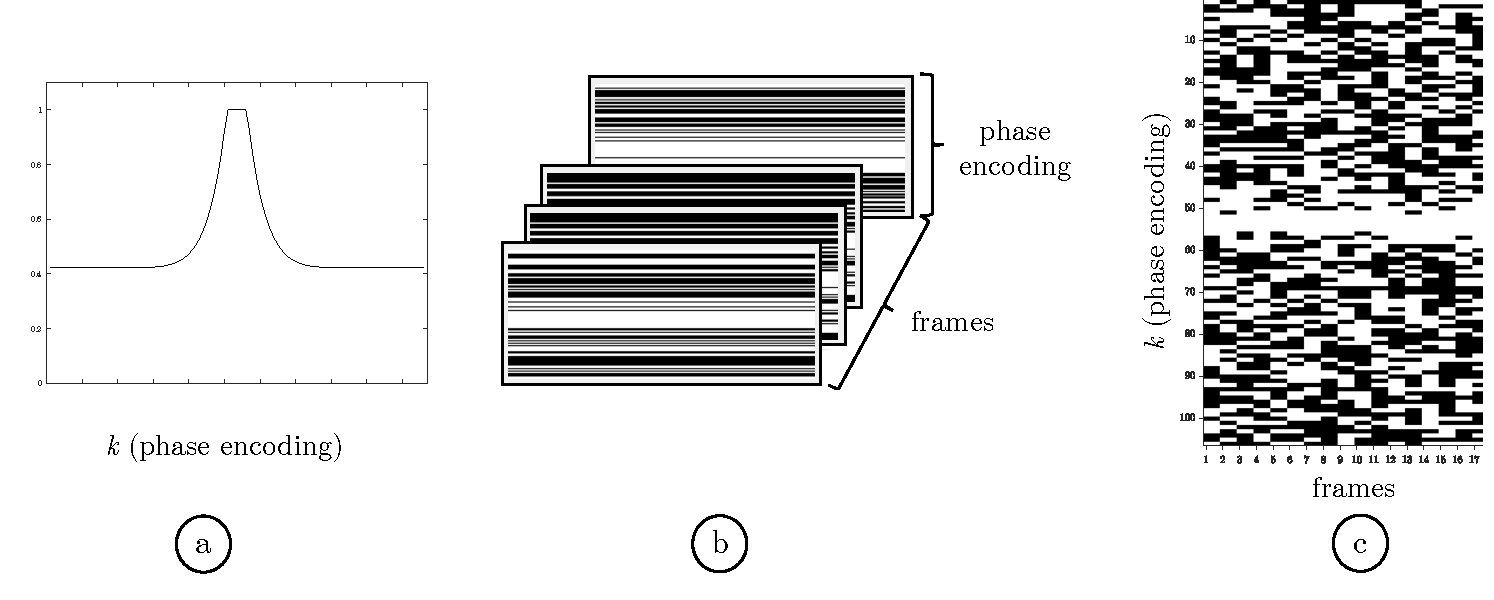
\includegraphics[width=0.9\textwidth]{Figures/CS1_1.pdf}
\caption[The probability density function, two times undersampled pattern for selected temporal frames and combined phase encode/temporal frame undersampling pattern]{The PDF from which the random undersampled phase encode (PE) pattern is drawn (a); CS\textit{-factor} $\times 2$ undersampling pattern for selected temporal frames with different patterns for each: black indicates not acquired, white indicates the acquired PE line (b); combined phase encode/temporal frame undersampling pattern (c).}
\label{fig: CS2}
\end{figure}
%*********************************************************
This method ensured dense sampling at the center of $k_y$ with decreasing $k_y$ density toward the edges of $k_y$ space~\cite{RNCS10}. 
Dense sampling at the center has been established as providing better CS reconstructed images than uniform random undersampling~\cite{Lustig:2007cua, RNCS9}.
%-new paragraph-%

%-new paragraph-%
The undersampling pattern for each temporal frame of the dynamic series was an independent random pattern (Figures~\ref{fig: CS2}b~and~\ref{fig: CS2}c) selected as recommended by Lustig~\cite{Lustig:2007cua}. 
In brief, an impulse at the origin in a 1D image is Fourier transformed to give a constant image. 
This constant 1D image is undersampled by the chosen random pattern and then a 1D iFFT is performed to obtain the 1D image of the impulse. 
If no undersampling is performed, then the impulse is completely recovered while the undersampling results in side lobes which are quantified as the sum of the coefficients not including the origin (denoted as interference) in the 1D image reconstructed by undersampling. 
The undersampling pattern with the lowest value for the interference (from 100 iterations) was chosen in separate iterations for a temporal frame. 
Different combinations of compressed sensing acceleration factors (\mbox{CS\textit{-factor}}) and views per segment (VPS) were tested for both \textit{in-vitro} phantom as well as for \textit{in-vivo} calf muscle studies (Figure~\ref{fig: CS3}).
%*********************************************************
\begin{figure}[!htb]
\vspace{+0.2cm}
\centering
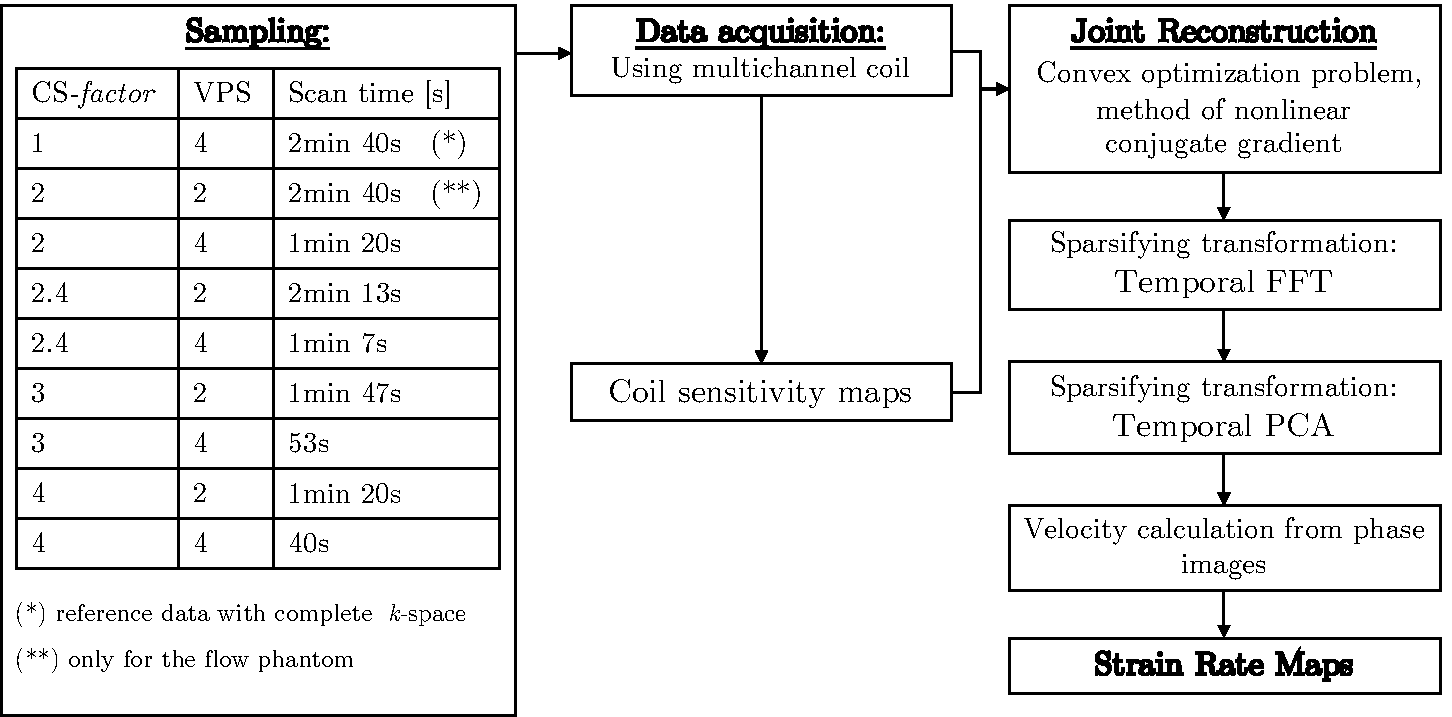
\includegraphics[width=0.9\textwidth]{Figures/CS1_2.pdf}
\caption[The $k_y$\textit{-t} SPARSE SENSE acquisition and reconstruction pipeline]{The $k_y$\textit{-t} SPARSE SENSE acquisition and reconstruction pipeline. Different sampling patterns and views per segment were tested to identify the highest acceleration factors that would still produce artifact free images after CS reconstruction. \mbox{\textit{k-}space} data was the input, the zero filled iFFT was the start point for the Temporal FFT.}
\label{fig: CS3}
\end{figure}
%*********************************************************
The undersampled patterns generated as detailed above were integrated into the velocity encoded FGRE sequence by modifying the proprietary pulse sequence (GE Medical Systems, version 15M4, WI, USA) using the EPIC programming environment. 
The undersampled mask for each temporal frame was read from an external file. 
The entire sequence was tested on the simulation platform as well as during run-time to verify that the undersampled patterns were correctly reproduced.

%`````````````````````````````````````````````````````````
\textit{Compressed sensing iterative reconstruction:}
%`````````````````````````````````````````````````````````
The flowchart for the iterative non-linear reconstruction algorithm is shown in Figure~\ref{fig: CS3} and follows the $k_y$\textit{-t} SPARSE SENSE method reported earlier~\cite{RNCS9, RNCS10, RNCS14}. 
Data was downloaded from the scanner as the complex \mbox{\textit{k-}space} data for each coil for each temporal frame. 
Data from the multiple channels was combined to form a self-calibrated coil sensitivity map $\mathbb{C}$. 
The coil sensitivity map is obtained by a temporal average over all the phases followed by an adaptive array combination~\cite{RNCS15}.
%-new paragraph-%

%-new paragraph-%
A two-stage process is used to reconstruct the image; the first stage uses the temporal Fourier transform as the sparsifying transform while the second stage uses the temporal PCA as the sparsifying transform (Figure~\ref{fig: CS3}). 
The starting point of the first stage (temporal FT as the sparsifying transform) is the sensitivity-weighted multicoil image combination of the zero-filled Fourier reconstruction of the undersampled data. 
A joint reconstruction is performed over all coils and all temporal frames. 
CS reconstruction minimizes the functional shown in Equation~\ref{eq: CS2}:
%.........................................................
\begin{equation}\label{eq: CS2}
f\left(\mathbf{I}\right) = \min_{\mathbf{I}} |{\mathcal{F}_{\mathrm{su}} \mathbb{C} \cdot \mathbf{I} - \mathbb{K}| _{2}^{2}} + \lambda_{\mathcal{F}/\mathcal{PCA}} |{\mathcal{W}_{\mathcal{F}/\mathcal{PCA}} \cdot \mathbf{I}}|_1
\end{equation}
%.........................................................
where $\mathbf{I}$ (current reconstructed image) and $\mathbb{K}$ (acquired undersampled \mbox{\textit{k-}space} data) are defined according to Equations~\ref{eq: CS3}~and~\ref{eq: CS4} respectively:
%.........................................................
\begin{equation}\label{eq: CS3}
\mathbf{I} = \begin{bmatrix} 
    \mathbf{i}_{11} & \dots & \mathbf{i}_{t1} \\
    \vdots & \ddots & \\
    \mathbf{i}_{1N} &        & \mathbf{i}_{tN} 
    \end{bmatrix}
\end{equation}
%.........................................................
%.........................................................
\begin{equation}\label{eq: CS4}
    \mathbb{K} =\mathcal{F}_{\mathrm{su}} \mathbb{C} \cdot \mathbf{I} = \begin{bmatrix} 
    \mathbf{k}_{11} & \dots & \mathbf{k}_{t1} \\
    \vdots & \ddots & \\
    \mathbf{k}_{1N} &        & \mathbf{k}_{tN} 
    \end{bmatrix}
\end{equation}
%.........................................................
with $N$ being the number of coils and $t$, the number of temporal frames and $\mathcal{F}_{\mathrm{su}}$ and $\mathbb{C}$ are the spatially undersampled Fourier operator and coil sensitivity vector respectively defined by Equations~\ref{eq: CS5}:
%.........................................................
\begin{equation}\label{eq: CS5}
    \mathcal{F}_{\mathrm{su}} = \begin{bmatrix} 
    \mathrm{F_{su}}^{1} \\
    \vdots \\
    \mathrm{F_{su}}^{t}
    \end{bmatrix} , \quad \mathbb{C} = \left[ \mathrm{C}_1 \dots \mathrm{C}_N \right]
\end{equation}
%.........................................................
The functional in Equation~\ref{eq: CS1} was minimized using a nonlinear conjugate gradient method~\cite{Lustig:2007cua}. 
The $\ell_1$ norm term (second term on LHS) maximizes the sparsity in the transform domain, $\mathcal{W}_{\mathcal{F}/\mathcal{PCA}}$ is the sparsifying transform (temporal FT in the first stage and PCA in the second stage of CS reconstruction), the $\ell_2$ norm (first term on LHS) ensures data fidelity between the estimated image and the acquired data, and $\lambda_{\mathcal{F}/\mathcal{PCA}}$ is the regularization parameter whose value controls the balance between image sparsity and image fidelity.
%-new paragraph-%

%-new paragraph-%
The CS reconstruction was performed offline using in-house built software developed in MATLAB (version R2018b. The MathWorks Inc. MA, USA) running on macOS (version 10.14.5 Apple Inc. CA, USA). 
Using a computer with Intel Core i5 CPU at $\SI{3.5}{\giga\hertz}$ with $\SI{16}{\gibi\byte}$ global memory, the total computational time was $\sim \SI{30}{\minute}$ for each series.
%-new paragraph-%

%-new paragraph-%
%`````````````````````````````````````````````````````````
\textit{Optimization:}
%`````````````````````````````````````````````````````````
 The regularization parameters $\lambda$ and the number of iterations for the temporal FT and for the temporal PCA of the CS reconstruction were optimized independently for the flow phantom data and for the muscle data. 
 The acquired undersampled images were used for phantom optimization while simulated undersampled images were used in the muscle data optimization. 
 The latter choice was based on the fact that comparing the reference to the acquired undersampled images may be biased by small differences in the contraction patterns in two separate acquisitions. 
 Optimization was performed to minimize the Root Mean Square Error (RMSE) in velocity estimated from the difference between the velocity from the full \mbox{\textit{k-}space} and from the undersampled \mbox{\textit{k-}space} data. 
 For the phantom, the velocity was estimated in the three flow tubes while for the muscle data, the velocity was estimated in a region of interest (ROI) [20 pixels $\times$ 7 pixels $= \SI{23}{\milli\meter} \times \SI{8}{\milli\meter}$] placed in the medial gastrocnemius. 
 The optimization was performed for each CS acceleration factor stepping through a grid of values for $\lambda$ and the number of iterations in the following range: 
%.........................................................
\begin{align}\label{eq: CS6}
\lambda_{\mathcal{F}} = \left[ 0.01, 0.10\right], \Delta_{\lambda} = 5\times10^{-3} \qquad & \mathcal{F}_\text{ite} = [10;30], \Delta_{\text{ite}}=5 \\
\lambda_{\mathcal{PCA}} = \left[ 0, 0.10\right], \Delta_{\lambda} = 5\times10^{-3} \qquad & \mathcal{PCA}_\text{ite} = [10;30], \Delta_{\text{ite}}=5 
\end{align}
%.........................................................
%---------------------------------------------------------
\subsubsection{Static and flow phantom}
%---------------------------------------------------------
Three tubes (diameter of 1cm) with constant flow were wound around a static water phantom such that the flow in the tubes was perpendicular to the image plane and opposite to each other (Figure~\ref{fig: CSS1}a-d).
%*********************************************************
\begin{figure}[!htb]
\vspace{+0.2cm}
\centering
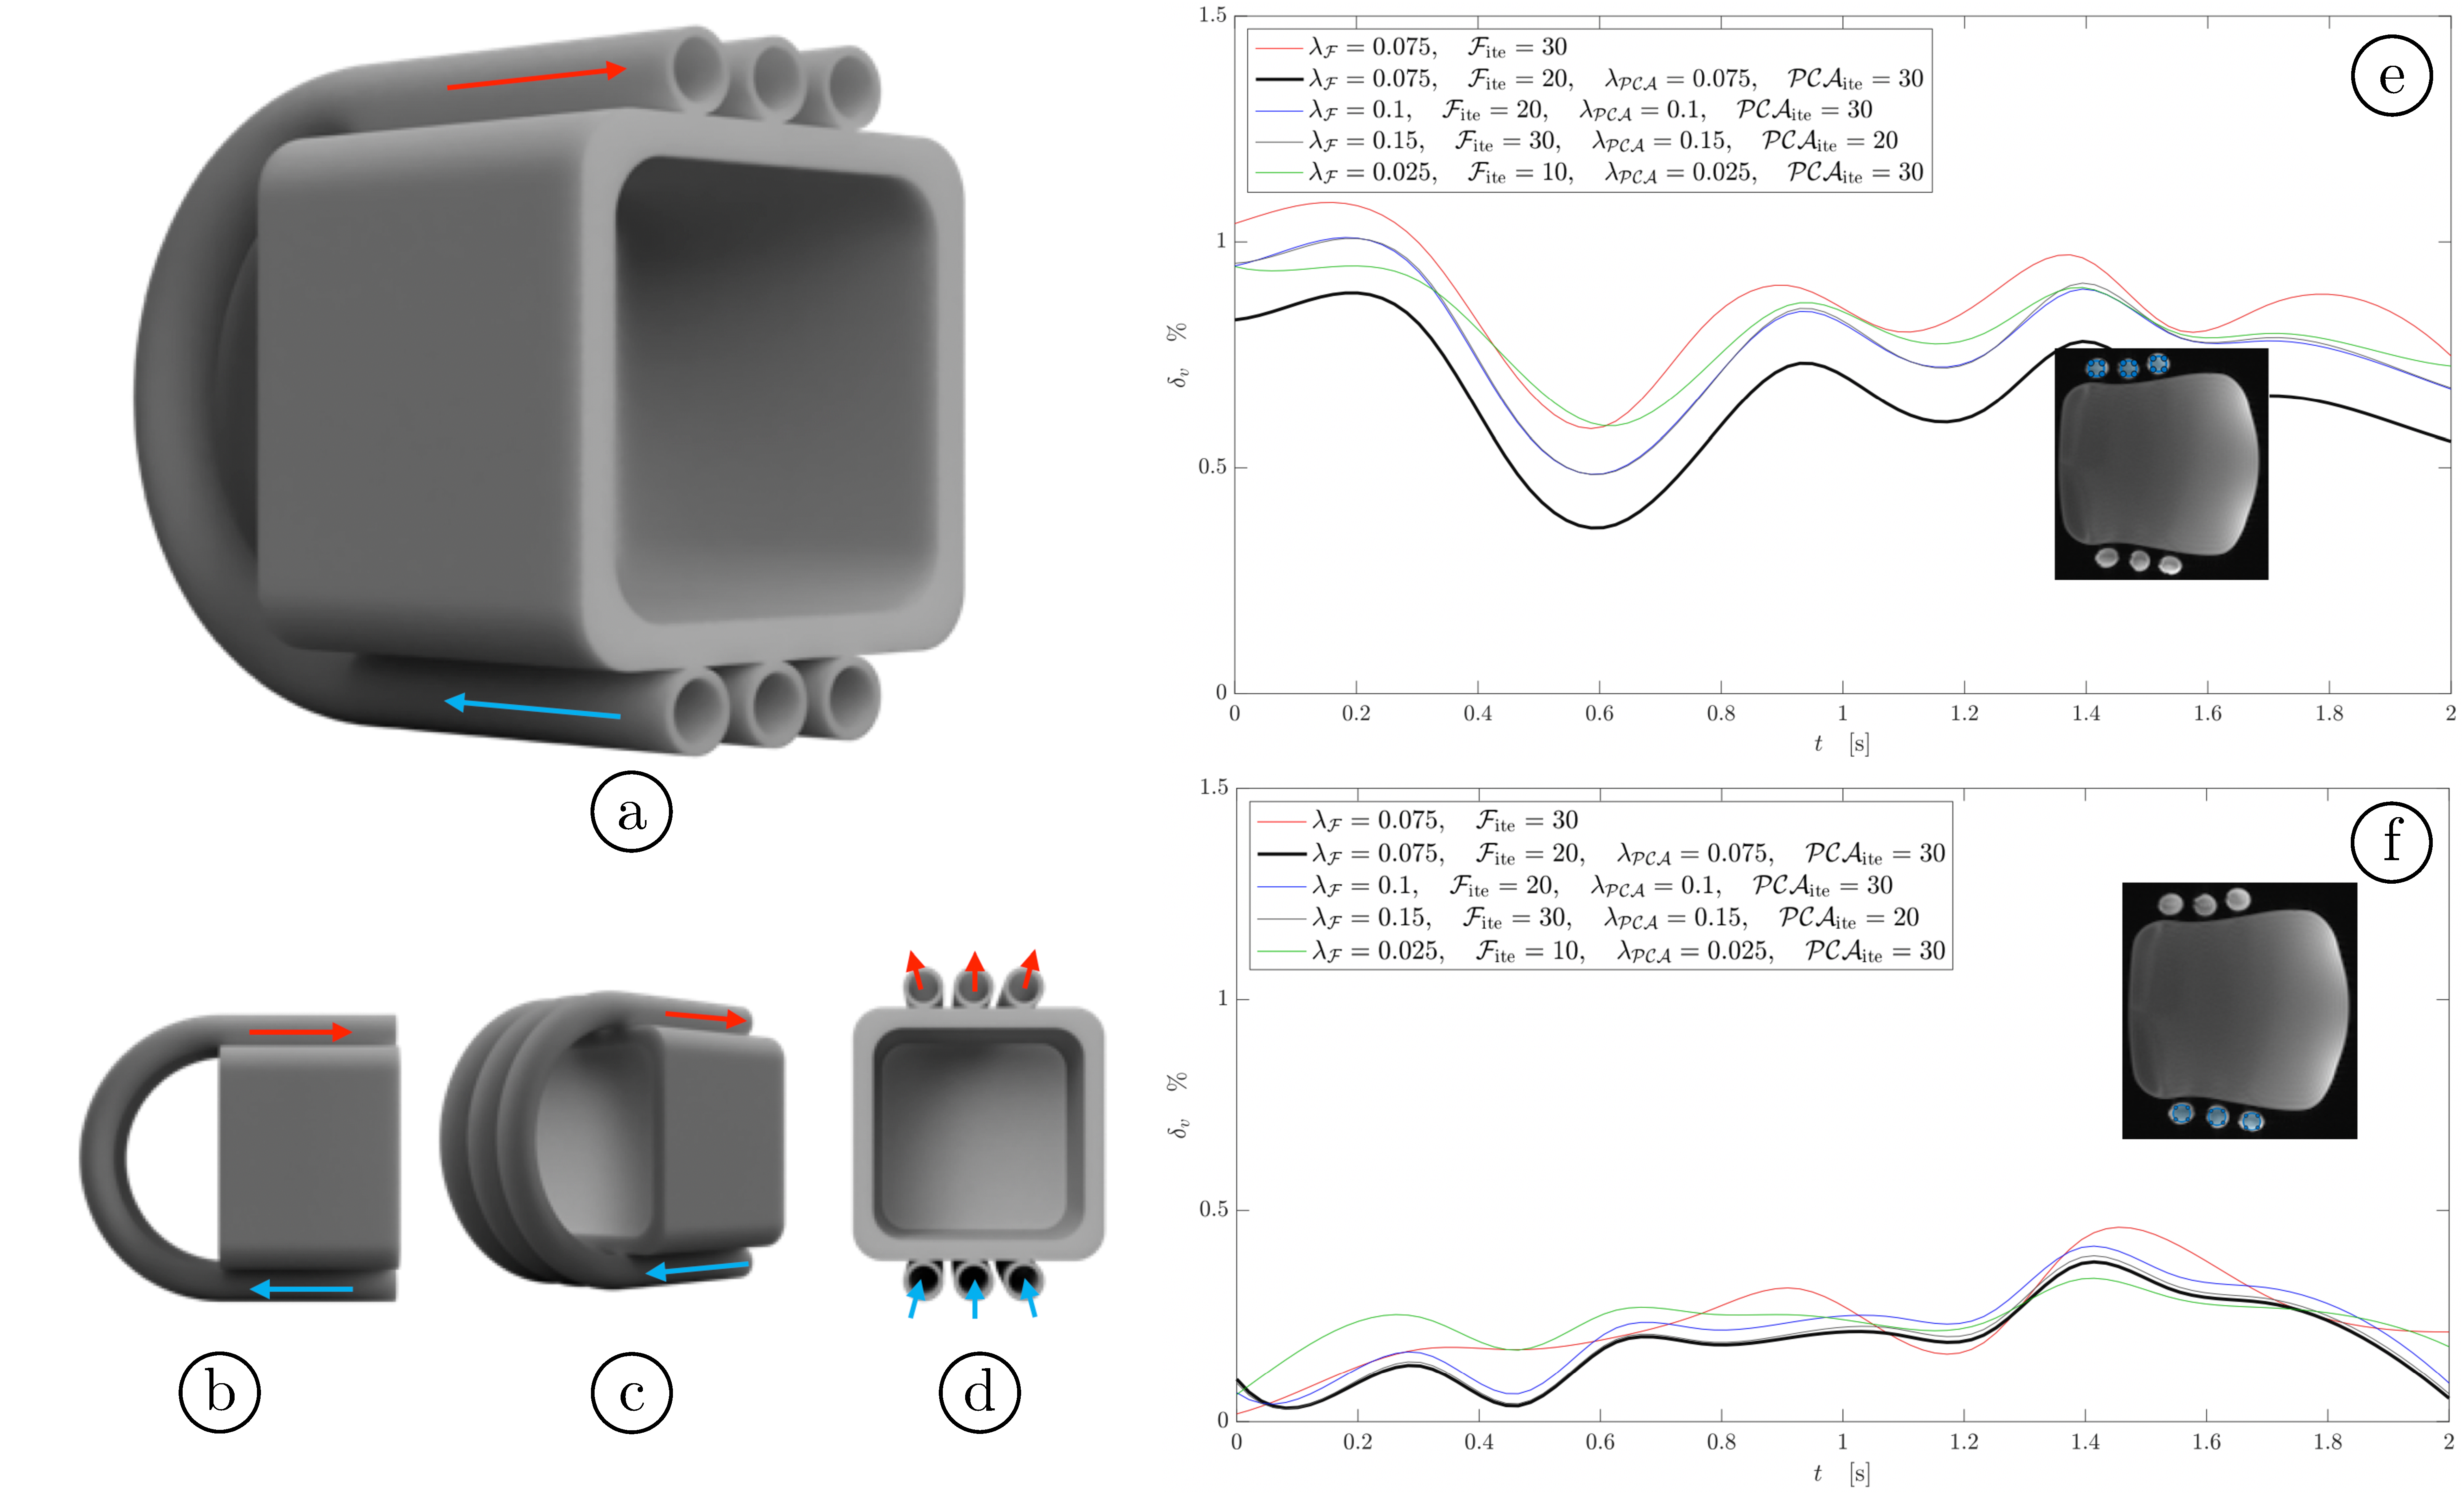
\includegraphics[width=1\textwidth]{Figures/CS1_3.pdf}
\caption[Rendering of the constant flow phantom and optimization plots]{Rendering of the constant flow phantom used to validate velocities calculated from the CS reconstructed images (a - d). Water flow directions are denoted by arrows. Velocity measurements were performed in the axial orientation (d). Optimization plots (e) for flow in the anterior and (f) posterior tubes for few best combinations.}
\label{fig: CSS1}
\end{figure}
%*********************************************************
Axial slices were acquired ensuring that the flow through the tubes was orthogonal to the plane of the image. 
The static/flow phantom was imaged with the full \mbox{\textit{k-}space} acquisition and with the undersampled acquisitions (eight different combinations of CS acceleration factors and views per segment). 
Three different in-flow velocities were set for the phantom: 2.5, 5 and $\SI{7.5}{\centi\meter/\second}$ and verified using the flowmeter~1G08~R3 (Cole-Parmer, IL, USA) resulting in 6 different (3 velocity magnitudes $\times$ 2 opposite directions $= 6$) flow velocities available for measurements using VEPC images.
%---------------------------------------------------------
\subsubsection{\textit{In-vivo} human subject imaging: }
%---------------------------------------------------------
Eleven subjects (5 male and 6 female) were included in this study after written informed consent had been obtained. 
The criterion for inclusion was that subjects should be moderately active and those with any surgical procedures performed on the lower leg were excluded. 
All subjects were normal, healthy volunteers. 
The study was carried out under the approval of the Medical Research Ethics Board of UC San Diego, and conformed to all standards for the use of human subjects in research as outlined in the Declaration of Helsinki on the use of human subjects in research.
%-new paragraph-%

%-new paragraph-%
Magnetic resonance imaging was performed on a $\SI{1.5}{\tesla}$ Signa HD16 MR scanner (GE Medical Systems, WI, USA), with the subject lying supine, feet first, with the right leg (i.e., the dominant leg to be imaged) resting against foot pedal~\cite{RNSS10}. 
An optical fiber pressure transducer was glued to the foot pedal placed inside 8-channel radiofrequency coil. 
Pressure exerted against the foot pedal during isometric contraction was detected by the transducer, converted to a voltage by a spectrometer (Luna Innovations, VA, USA), and used to trigger the MR image acquisition using in-house built software developed in LabVIEW (National Instruments Inc, TX, USA). 
For data analysis, the voltage output from the pressure transducer was later converted into units of force [$\SI{}{\newton}$] based on a calibration of the system using disc weights. 
Images were acquired during submaximal, isometric contraction at 35\% of the individual maximum voluntary isometric contraction (MVIC). 
The MR image acquisition was completed in approximately 53 cycles for the full \mbox{\textit{k-}space} acquisition and the number of cycles ranged from 44 to 13 cycles for the accelerated scans; thus, it was important to ensure consistency of motion. 
This was ensured by providing the subject with real-time visual feedback of the actual force generated by the subject superposed on the target force curve to facilitate consistent contractions~\cite{Malis:2018fr}.
%---------------------------------------------------------
\subsubsection{Magnetic resonance imaging}
%---------------------------------------------------------
The MR images used in this report included a localizer scan to identify the oblique sagittal orientation that best depicted the fascicles in the medial gastrocnemius. 
The acquisition parameters for the reference full \mbox{\textit{k-}space} VEPC acquisition was: echo time (TE):~$\SI{7.7}{\milli\second}$, repetition time (TR):~$\SI{17.8}{\milli\second}$, signal averages (NEX):~2, flip angle (FA):~$\SI{20}{\degree}$, slice thickness:~$\SI{5}{\milli\meter}$, field of view (FOV):~$\SI{30}{\centi\meter} \times \SI{22.5}{\centi\meter}$ (partial phase FOV: 0.55), matrix:~$256 \times 192$ (lower resolution in the phase direction), 4 views per segment (VPS), 3~slices, 17~temporal frames (with view sharing factor = 2), $\SI{10}{\centi\meter/\second}$ 3D velocity encoding. 
This resulted in 53 repetitions [192 (phase encode) $\times$ 2 (averages) $\times$ 0.55 (phase FOV)) / 4 (views per segment) = $53$] for each slice acquisition. 
The temporal resolution is calculated as: 17.8(TR) $\times$ 4 (VPS) $\times$ 4 (3 velocity encoding directions + 1 flow compensated) / 2 (view sharing) $ = \SI{142}{\milli\second}$. 
Seventeen temporal frames were collected within each isometric contraction-relaxation cycle of $\sim \SI{2.4}{\second}$ $(17 \times \SI{142}{\milli\second}  = \SI{2.4}{\milli\second})$. 
It should be noted that, in the reference sequence, the actual acquired number of temporal frames is only 8 with an acquired temporal resolution of $\SI{285}{\milli\second}$. 
For all the undersampled sequences, the geometry parameters were the same as in the original sequence while the number of phase-encode steps was decreased by the CS acceleration factors between 2 to 4 while varying views per segment between 2 and 4 as well. 
It should be noted that views per segment of 2 in the CS acquisitions increased the acquired temporal resolution by a factor of 2 compared to full \mbox{\textit{k-}space} acquisition (4 views per segment). 
The maximum \mbox{CS\textit{-factor}} achievable was determined from a simulation of a full \mbox{\textit{k-}space} data of muscle contraction. 
%-new paragraph-%

%-new paragraph-%
Flow phantom acquisition parameters were same as for the human scans with the only difference being that the cycle length was $\SI{2}{\second}$ resulting in 14 temporal frames.
%---------------------------------------------------------
\subsubsection{Image and Statistical Analysis}
%---------------------------------------------------------
Phase images were corrected for phase shading (mean background phase error) and denoised with a 2D anisotropic diffusion filter~\cite{RNCS17} to yield the velocity images. 
Phase shading was estimated by averaging all of the dynamic images in the cine sequence. 
This was based on the assumption that the net change in position (and therefore net velocity) over the isometric contraction-relaxation cycle was zero. 
The average image was subtracted from the phase image at each temporal frame. 
%-new paragraph-%

%-new paragraph-%
The ($2 \times 2$) SR tensor was calculated from the spatial gradient of the velocity images and then diagonalized to obtain the eigenvalues and eigenvectors~\cite{RNS16, Malis:2018fr}. 
Eigenvalues ($SR_{\mathrm{fiber}}$, $SR_{\mathrm{in-plane}}$) were sorted on a voxel basis. 
$SR_{\mathrm{fiber}}$ denotes deformation approximately along the muscle fiber long axis and is negative during muscle fiber shortening (contraction during phases 1-8 of reference VEPC sequence) and positive during relaxation (phases 9-17 of reference VEPC sequence). 
$SR_{\mathrm{in-plane}}$ denotes deformation in the muscle fiber cross-section and is positive during muscle fiber shortening and negative during relaxation.
%-new paragraph-%

%-new paragraph-%
Regions of interest were placed in the anterior and posterior tubes of the flow phantom were used to measure the velocity in the tubes for a range of flow in the phantom. 
Bland-Altman plots were used to analyze the velocities from the acquisitions with different VPS/CS combinations using the flowmeter velocity values as the reference. 
\textit{In-vivo} velocity and strain rate data were extracted and analyzed for the ROI [20px $\times$ 7px = $\SI{23}{\milli\meter}$ $\times$ $\SI{8}{\milli\meter}$] placed in the medial gastrocnemius. 
In order to ensure that the same anatomic region was sampled, each pixel in the ROI placed in the first temporal frame was tracked (with respect to the first frame) to locate the new pixel positions in successive frames, creating a frame-based ROI. 
Tracking was performed in 2D using the in-plane velocity information. 
The position in a subsequent frame was calculated based on the velocity information in the current frame. 
This allowed automated placement of an ROI in each frame that moved synchronously with the underlying anatomy. 
ROIs changed both location and shape (5 to 20\% in successive frames) but the number of points was kept constant to ensure average values were based on the same number of points/frame. 
Bland-Altman analysis was performed on strain rate data comparing that derived from reference full \mbox{\textit{k-}space} values to that obtained from undersampled sequences.
%~~~~~~~~~~~~~~~~~~~~~~~~~~~~~~~~~~~~~~~~~~~~~~~~~~~~~~~~~
\subsection{Results}
%~~~~~~~~~~~~~~~~~~~~~~~~~~~~~~~~~~~~~~~~~~~~~~~~~~~~~~~~~
Figure~\ref{fig: CSS2} shows, for one example subject, the average of the force measured in a full reference acquisition and for the undersampled acquisition (VPS/\mbox{CS\textit{-factor}}: $4/4$) over the contraction cycle. 
%*********************************************************
\begin{figure}[!htb]
\vspace{+0.2cm}
\centering
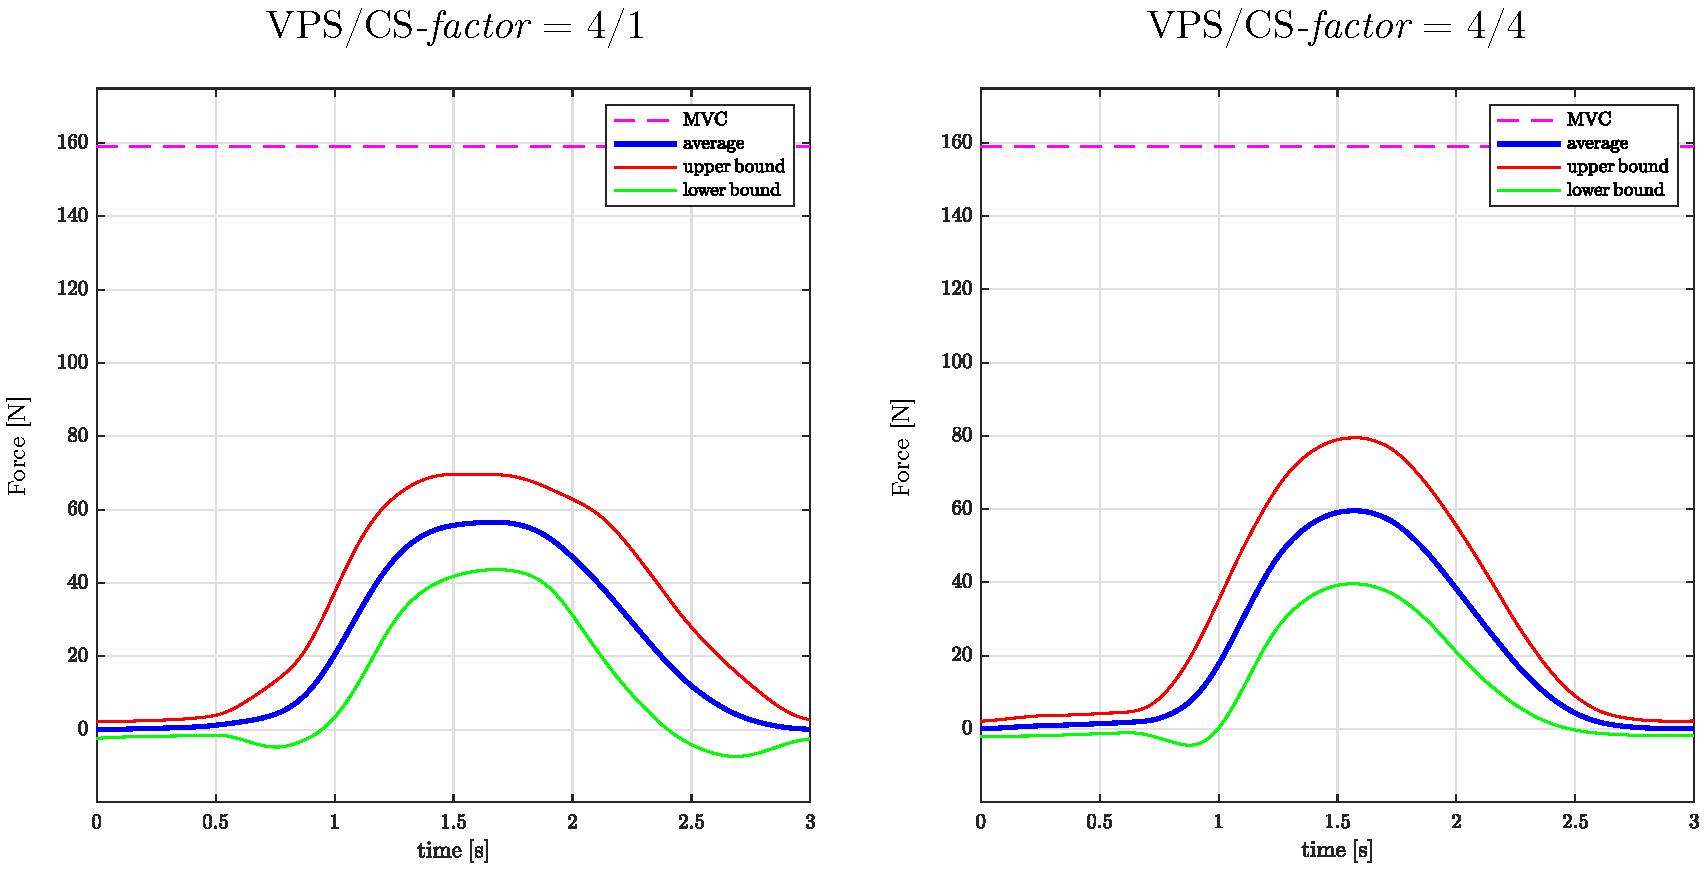
\includegraphics[width=\textwidth]{Figures/CS1_4.pdf}
\caption[Averaged force curve for the fully sampled acquisition and undersampled acquisition]{Averaged force curve with lower and upper boundary given as mean $\pm$ standard deviation for the fully sampled acquisition with 52 contractions cycles (left) and undersampled acquisition with 13 contractions cycles (right).}
\label{fig: CSS2}
\end{figure}
%*********************************************************
The upper and lower bound curves were generated by plotting points at mean $\pm$ standard deviation (SD) at each sampled point of the force output. 
While the range of upper and lower bound of the force during the contractions was not significantly different between the undersampled and full \mbox{\textit{k-}space}, the FWHM of the mean force is lower for the undersampled acquisition. 
Figure~\ref{fig: CSS3} shows an example velocity (phase) image from an undersampled acquisition (VPS/\mbox{CS\textit{-factor}}: $2/4$) and the denoised image after application of the 2D anisotropic diffusion filter. 
%*********************************************************
\begin{figure}[!htb]
\vspace{+0.2cm}
\centering
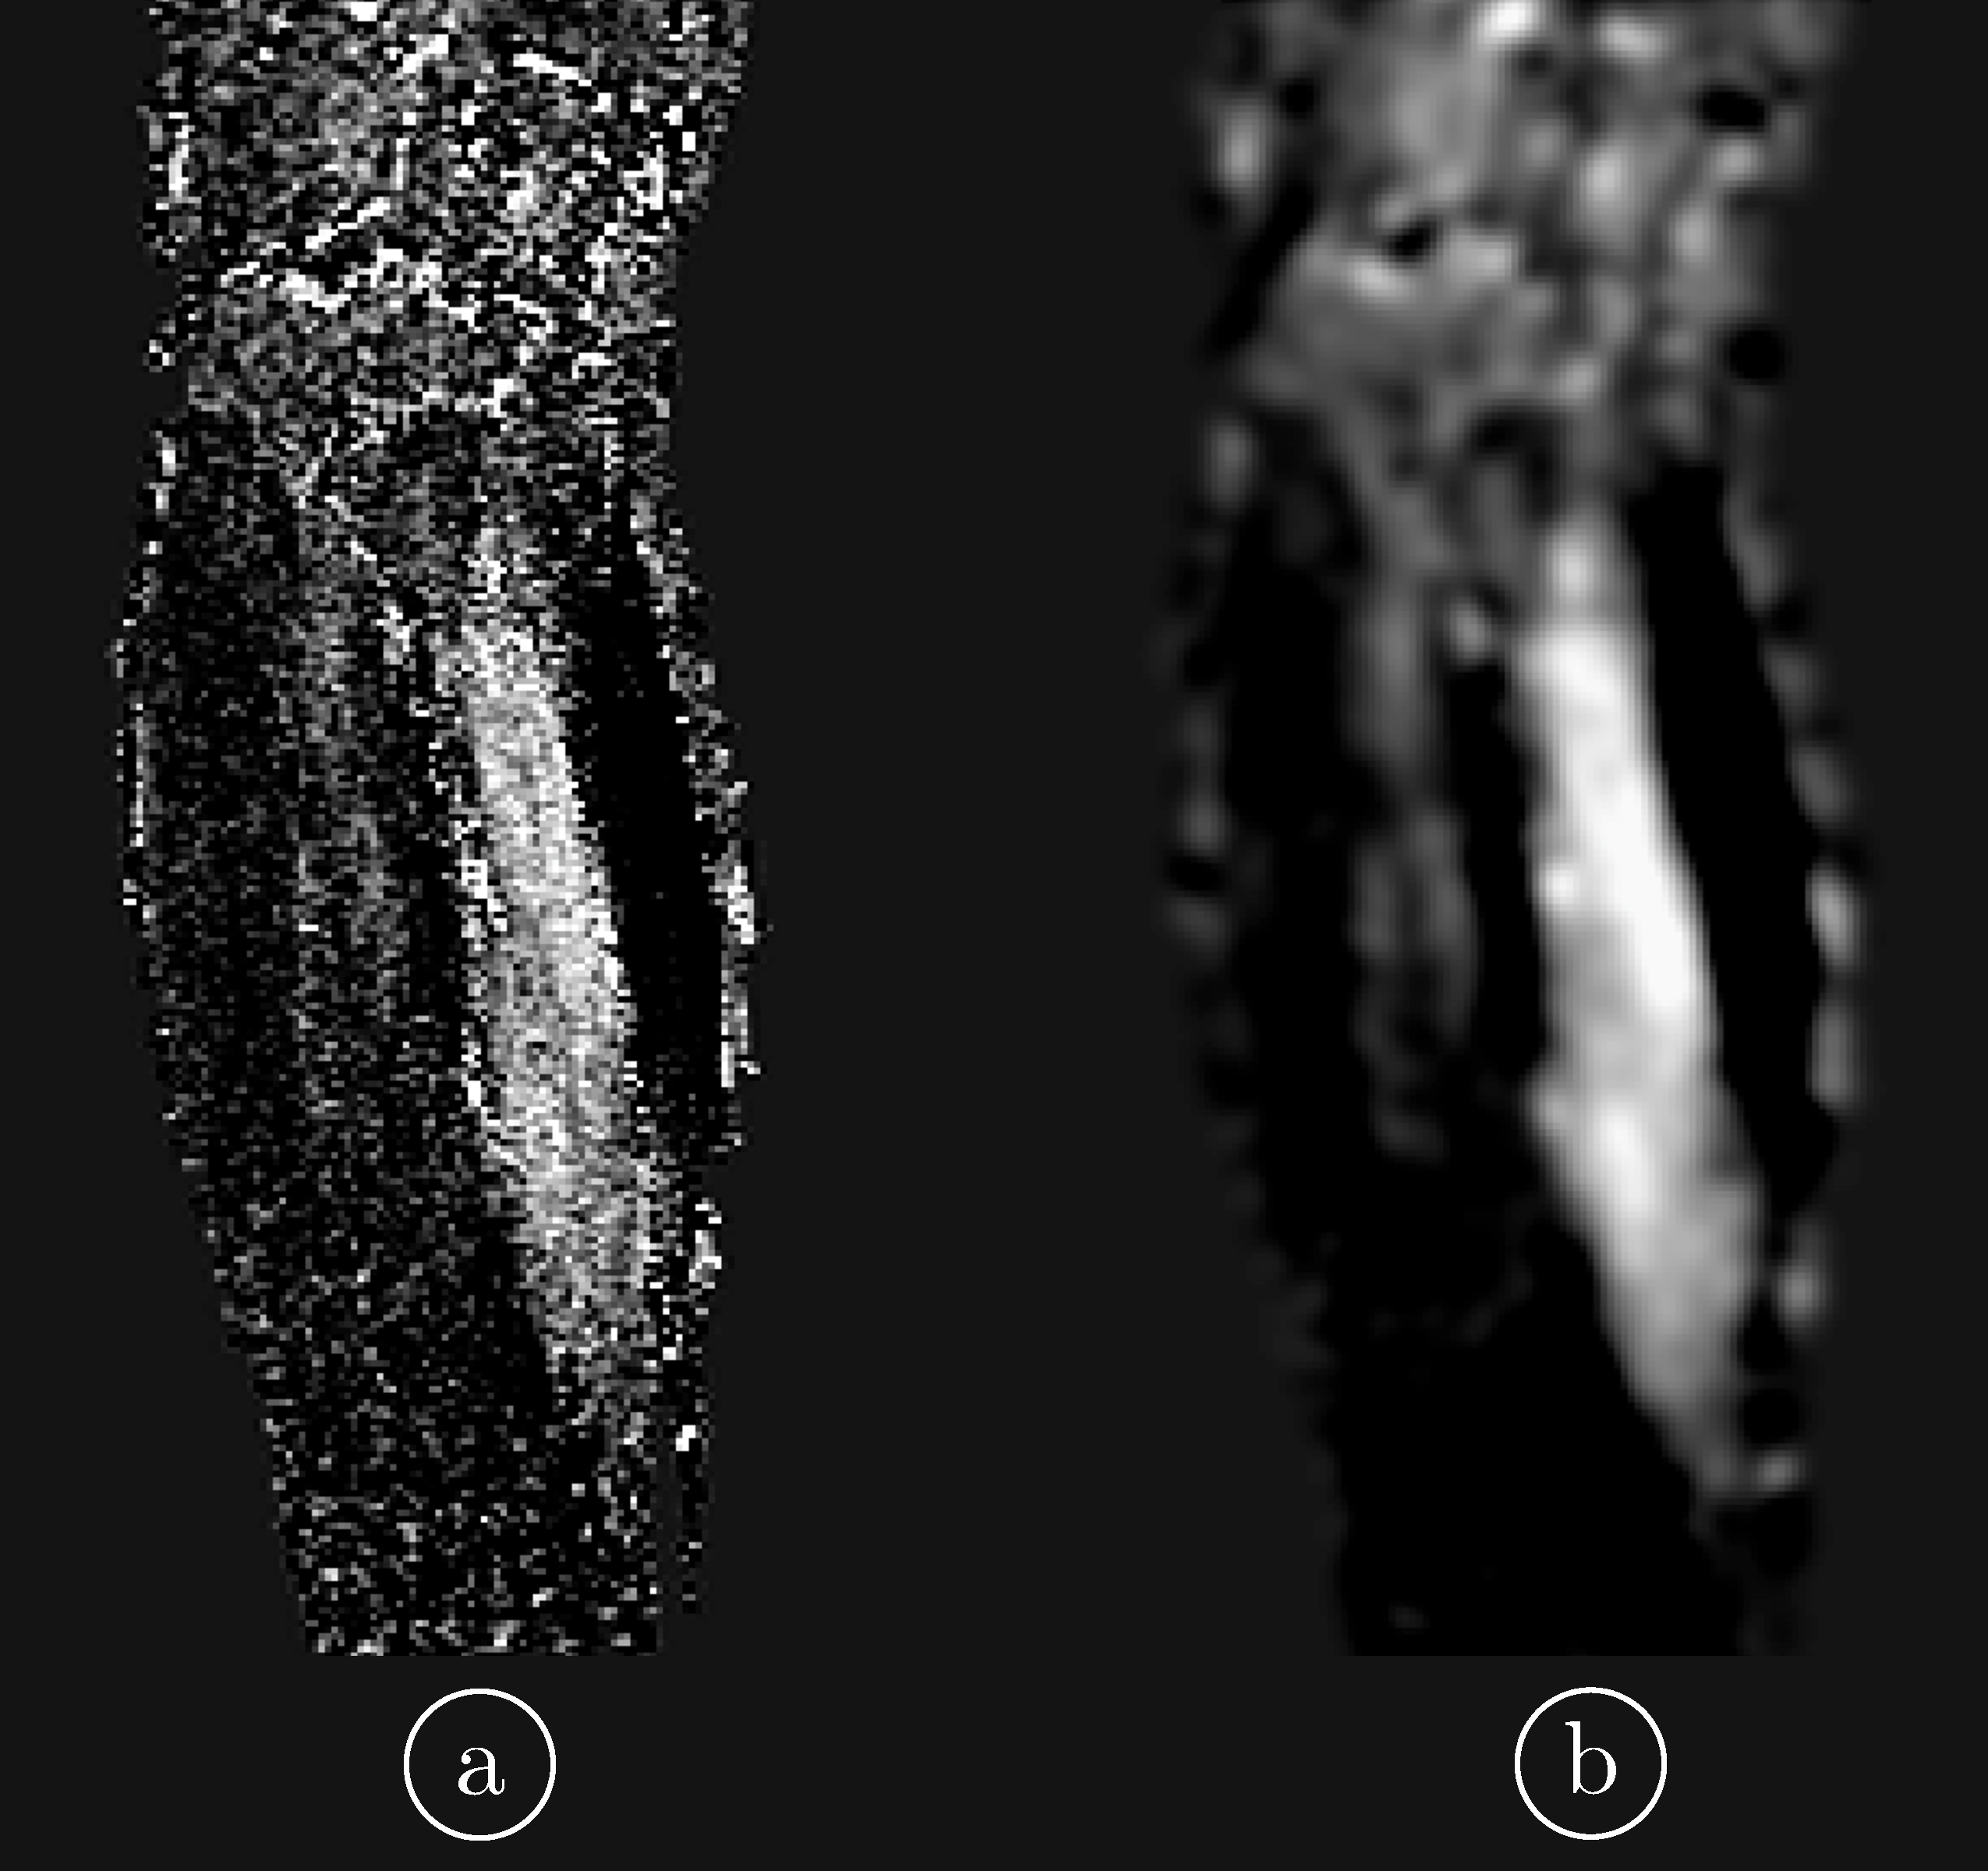
\includegraphics[scale=0.17]{Figures/CS1_5.pdf}
\caption[Velocity maps before and after 2D anisotropic diffusion filter]{Velocity maps before (a) and after (b) 2D anisotropic diffusion filter was applied for the frame corresponding to the peak of contraction cycle. Image shown on the left was acquired with a VPS/\mbox{CS\textit{-factor}} of 2/4. Parameters of anisotropic diffusion filter: $\kappa = 2$ , $\Delta = 1/7$  and 10 iterations.}
\label{fig: CSS3}
\end{figure}
%*********************************************************
The reduction in velocity (phase) noise is visually evident in the denoised image. 
Figure~\ref{fig: CSS4} shows the efficacy of the phase correction using the temporally averaged phase map on select frames of the dynamic cycle: the corrected frames show that the first and last frames are close to zero velocity (small discrepancies in the first and last frame arise from the fact the first frame is shifted compared to the start of the acquisition). 
%*********************************************************
\begin{figure}[!htb]
\vspace{+0.2cm}
\centering
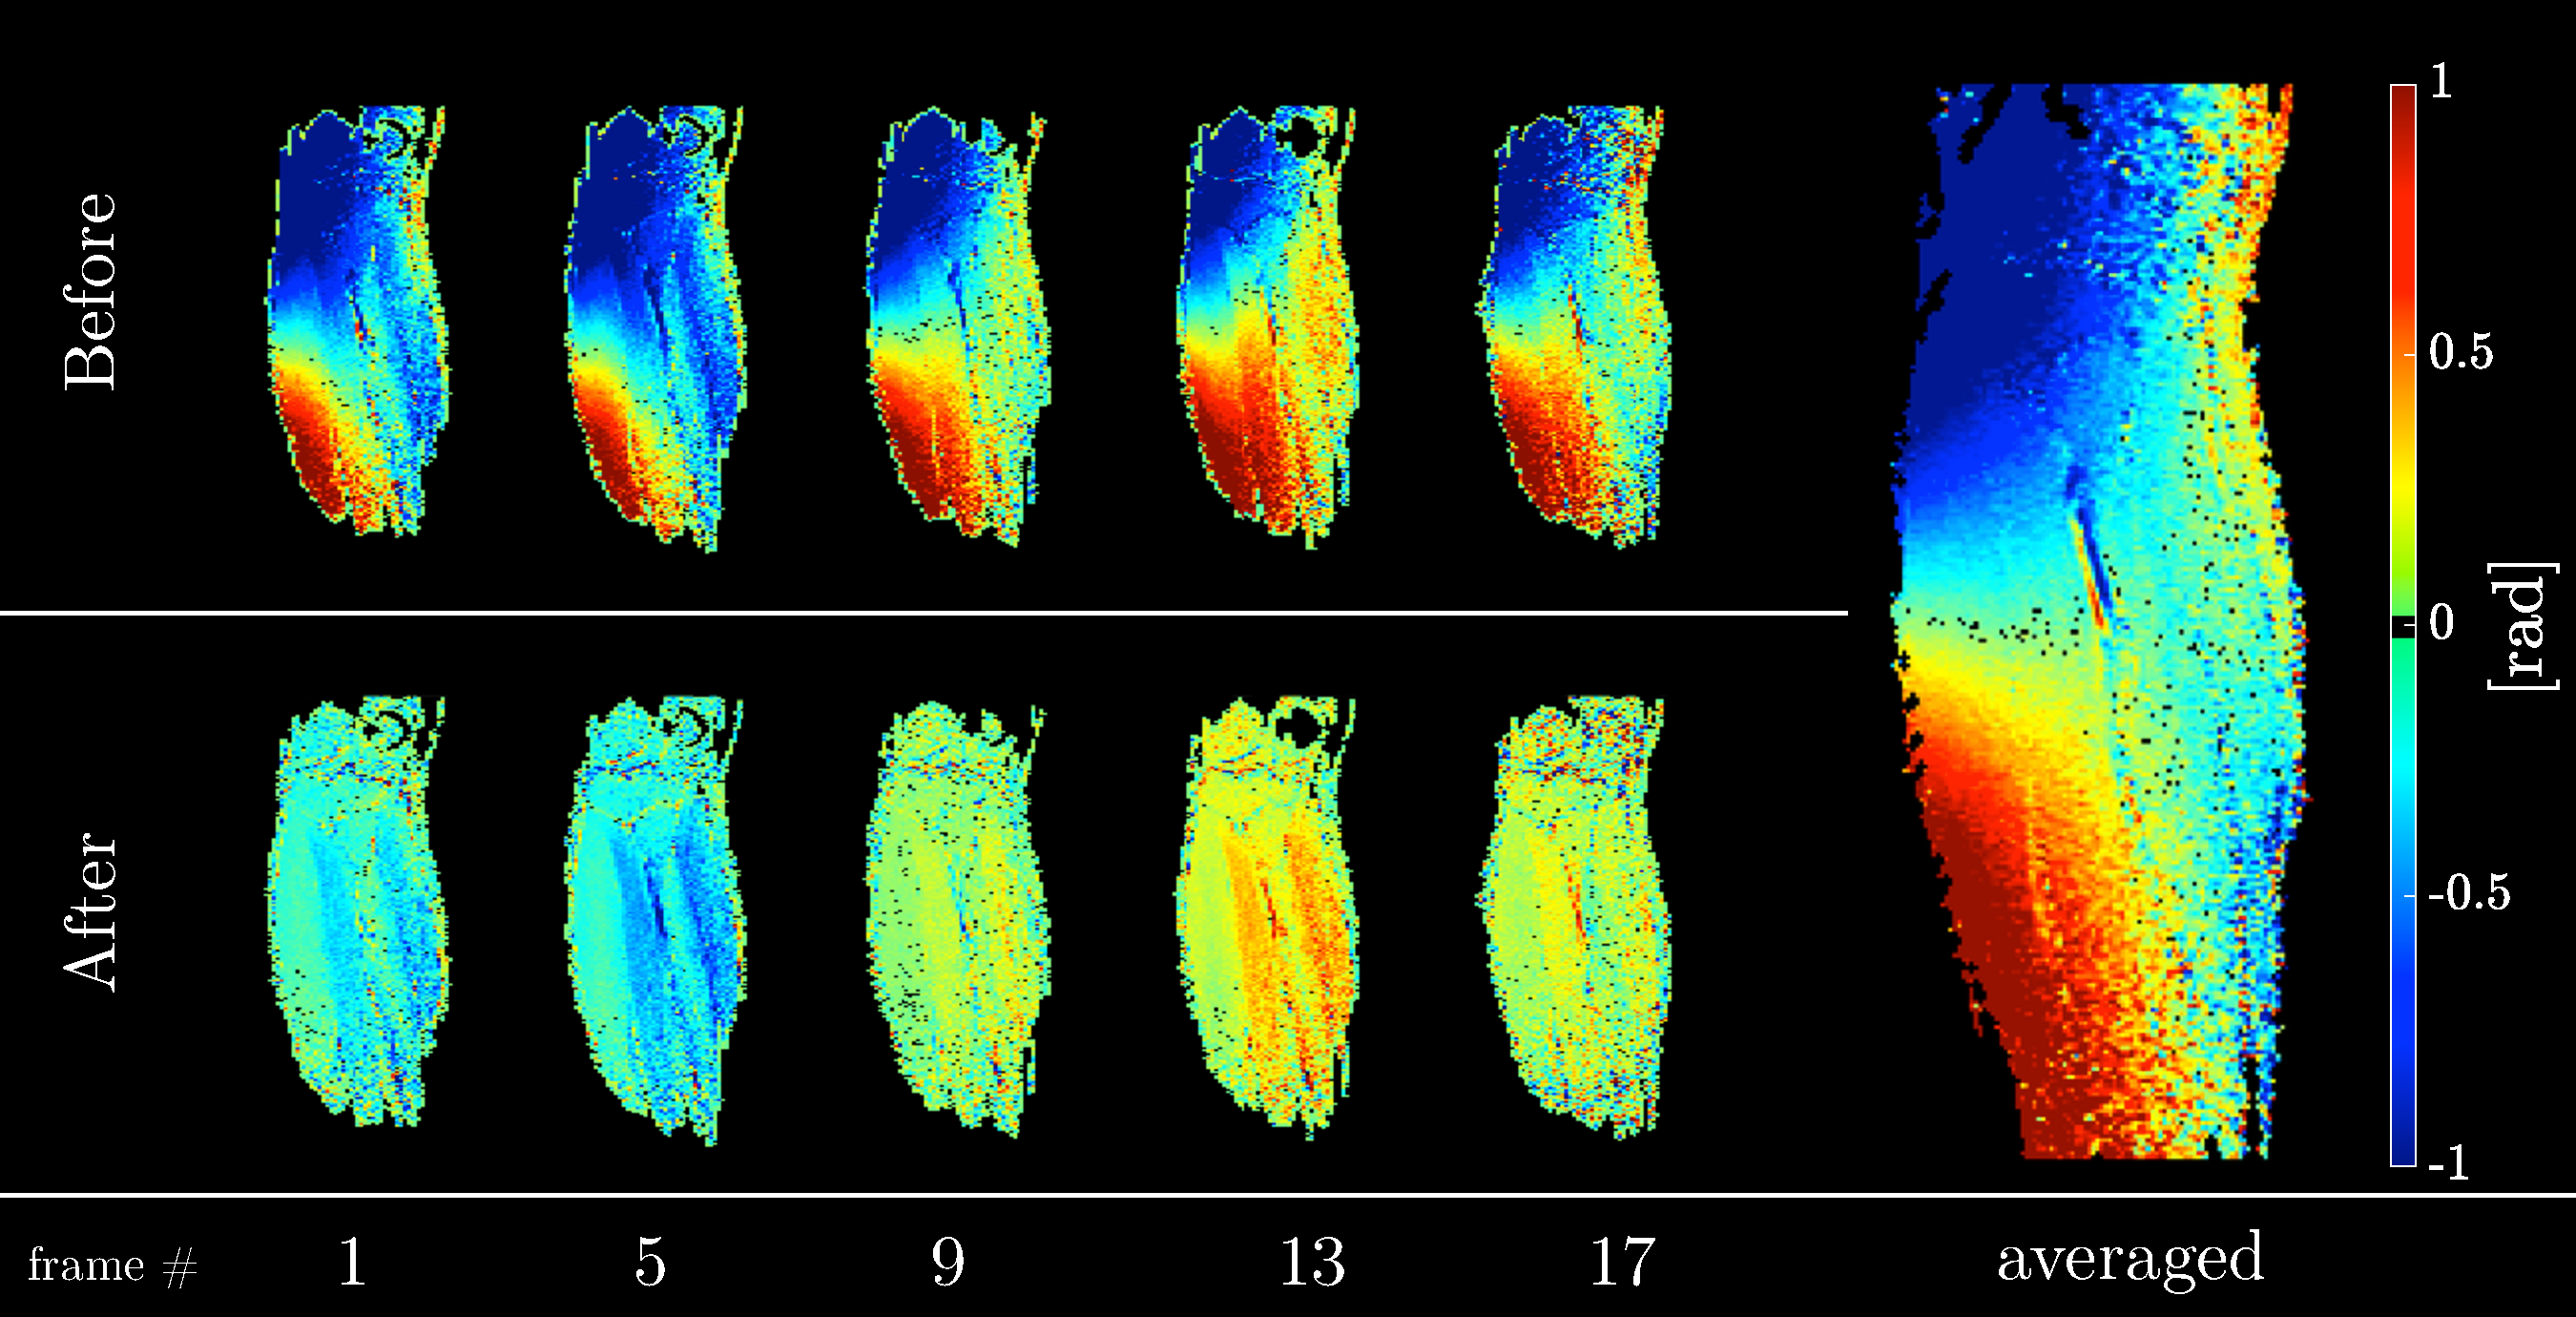
\includegraphics[width=0.9\textwidth]{Figures/CS1_6.pdf}
\caption[Selected frames of phase images for the direction of maximum velocity before and after correction for phase shading artifacts]{Selected frames of phase images for the direction of maximum velocity before (top row) and after (bottom row) correction for phase shading artifacts. The phase averaged image shown on the right is subtracted from each frame of the acquired images to generate the corrected images.}
\label{fig: CSS4}
\end{figure}
%*********************************************************
Two sparsifying transforms were used in the current study to improve image quality in the reconstructed images. 
The fully sampled dynamic magnitude data was undersampled in the $k_y$\textit{-t} plane to compare the sparsity provided by the temporal FT and temporal PCA transforms. 
Figure~\ref{fig: CS4} shows the images after the temporal FT and after the temporal PCA transform respectively and these images illustrate the higher sparsity of the PCA transform.
%*********************************************************
\begin{sidewaysfigure}
\vspace{+0.2cm}
\centering
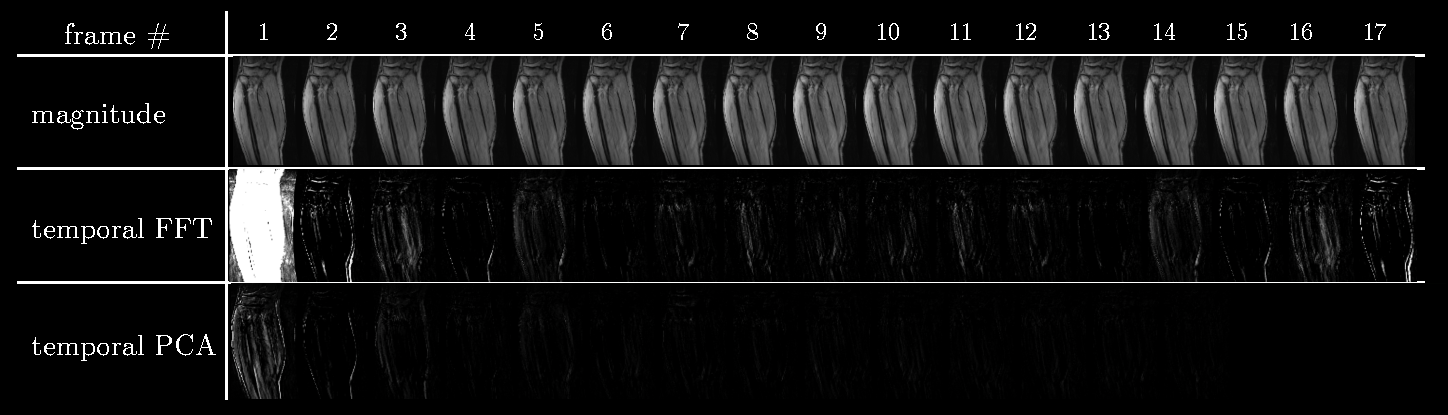
\includegraphics[width=8.5in]{Figures/CS1_7.pdf}
\captionsetup{width=8.5in}
\caption[Magnitude images and images after performing a temporal FFT and a temporal PCA transformations]{Magnitude images from a dynamic muscle scan based on the VEPC sequence: top row. Images after performing a temporal FFT (middle row) and a temporal PCA (bottom row) on the magnitude images. Middle (temporal FFT) and bottom (temporal PCA) have same intensity windowing.}
\label{fig: CS4}
\end{sidewaysfigure}
%*********************************************************
This is seen by the smaller number of images with non-zero coefficients in the PCA transform compared to the images in the FT transform. 
%-new paragraph-%

%-new paragraph-%
The results of the optimization of the regularization, $\lambda_{\mathcal{F}}$ and $\lambda_{\mathcal{PCA}}$ and iteration parameters for each stage using the phantom image data are shown in Figure~\ref{fig: CSS1}e,~f. 
Figure~\ref{fig: CSS1}e shows the optimization results for velocity estimated in the anterior tubes while Figure~\ref{fig: CSS1}f is the corresponding result for the tubes placed posteriorly. 
The root mean square of the difference (RMSE) in velocities (as a function of time in the dynamic cycle) measured in the constant flow phantom between reference full \mbox{\textit{k-}space} and undersampled \mbox{\textit{k-}space} was used as the metric for optimizing weights. 
The optimization was performed using undersampled data acquired with \mbox{CS\textit{-factor}} of 4, and VPS of 2. 
The plots are shown close to the minimum RMSE values since the total number of combinations of the parameters was large (503 combinations). 
At the optimal setting, the lowest values of 0.4\% was seen for the anterior tubes and $\sim 0.1\%$ for the posterior tubes confirming that the CS reconstruction was able to accurately reproduce velocities. 
The combination of values that minimized the RMSE was chosen as optimal and used for the rest of the phantom CS reconstructions. 
Figure~\ref{fig: CSS5} is the Bland-Altman plot of the velocities from the full \mbox{\textit{k-}space} acquisition and from undersampled acquisitions using 8 combinations of CS accelerations and VPS factors with the flowmeter values as the reference velocities. 
%*********************************************************
\begin{figure}[!htb]
\vspace{+0.2cm}
\centering
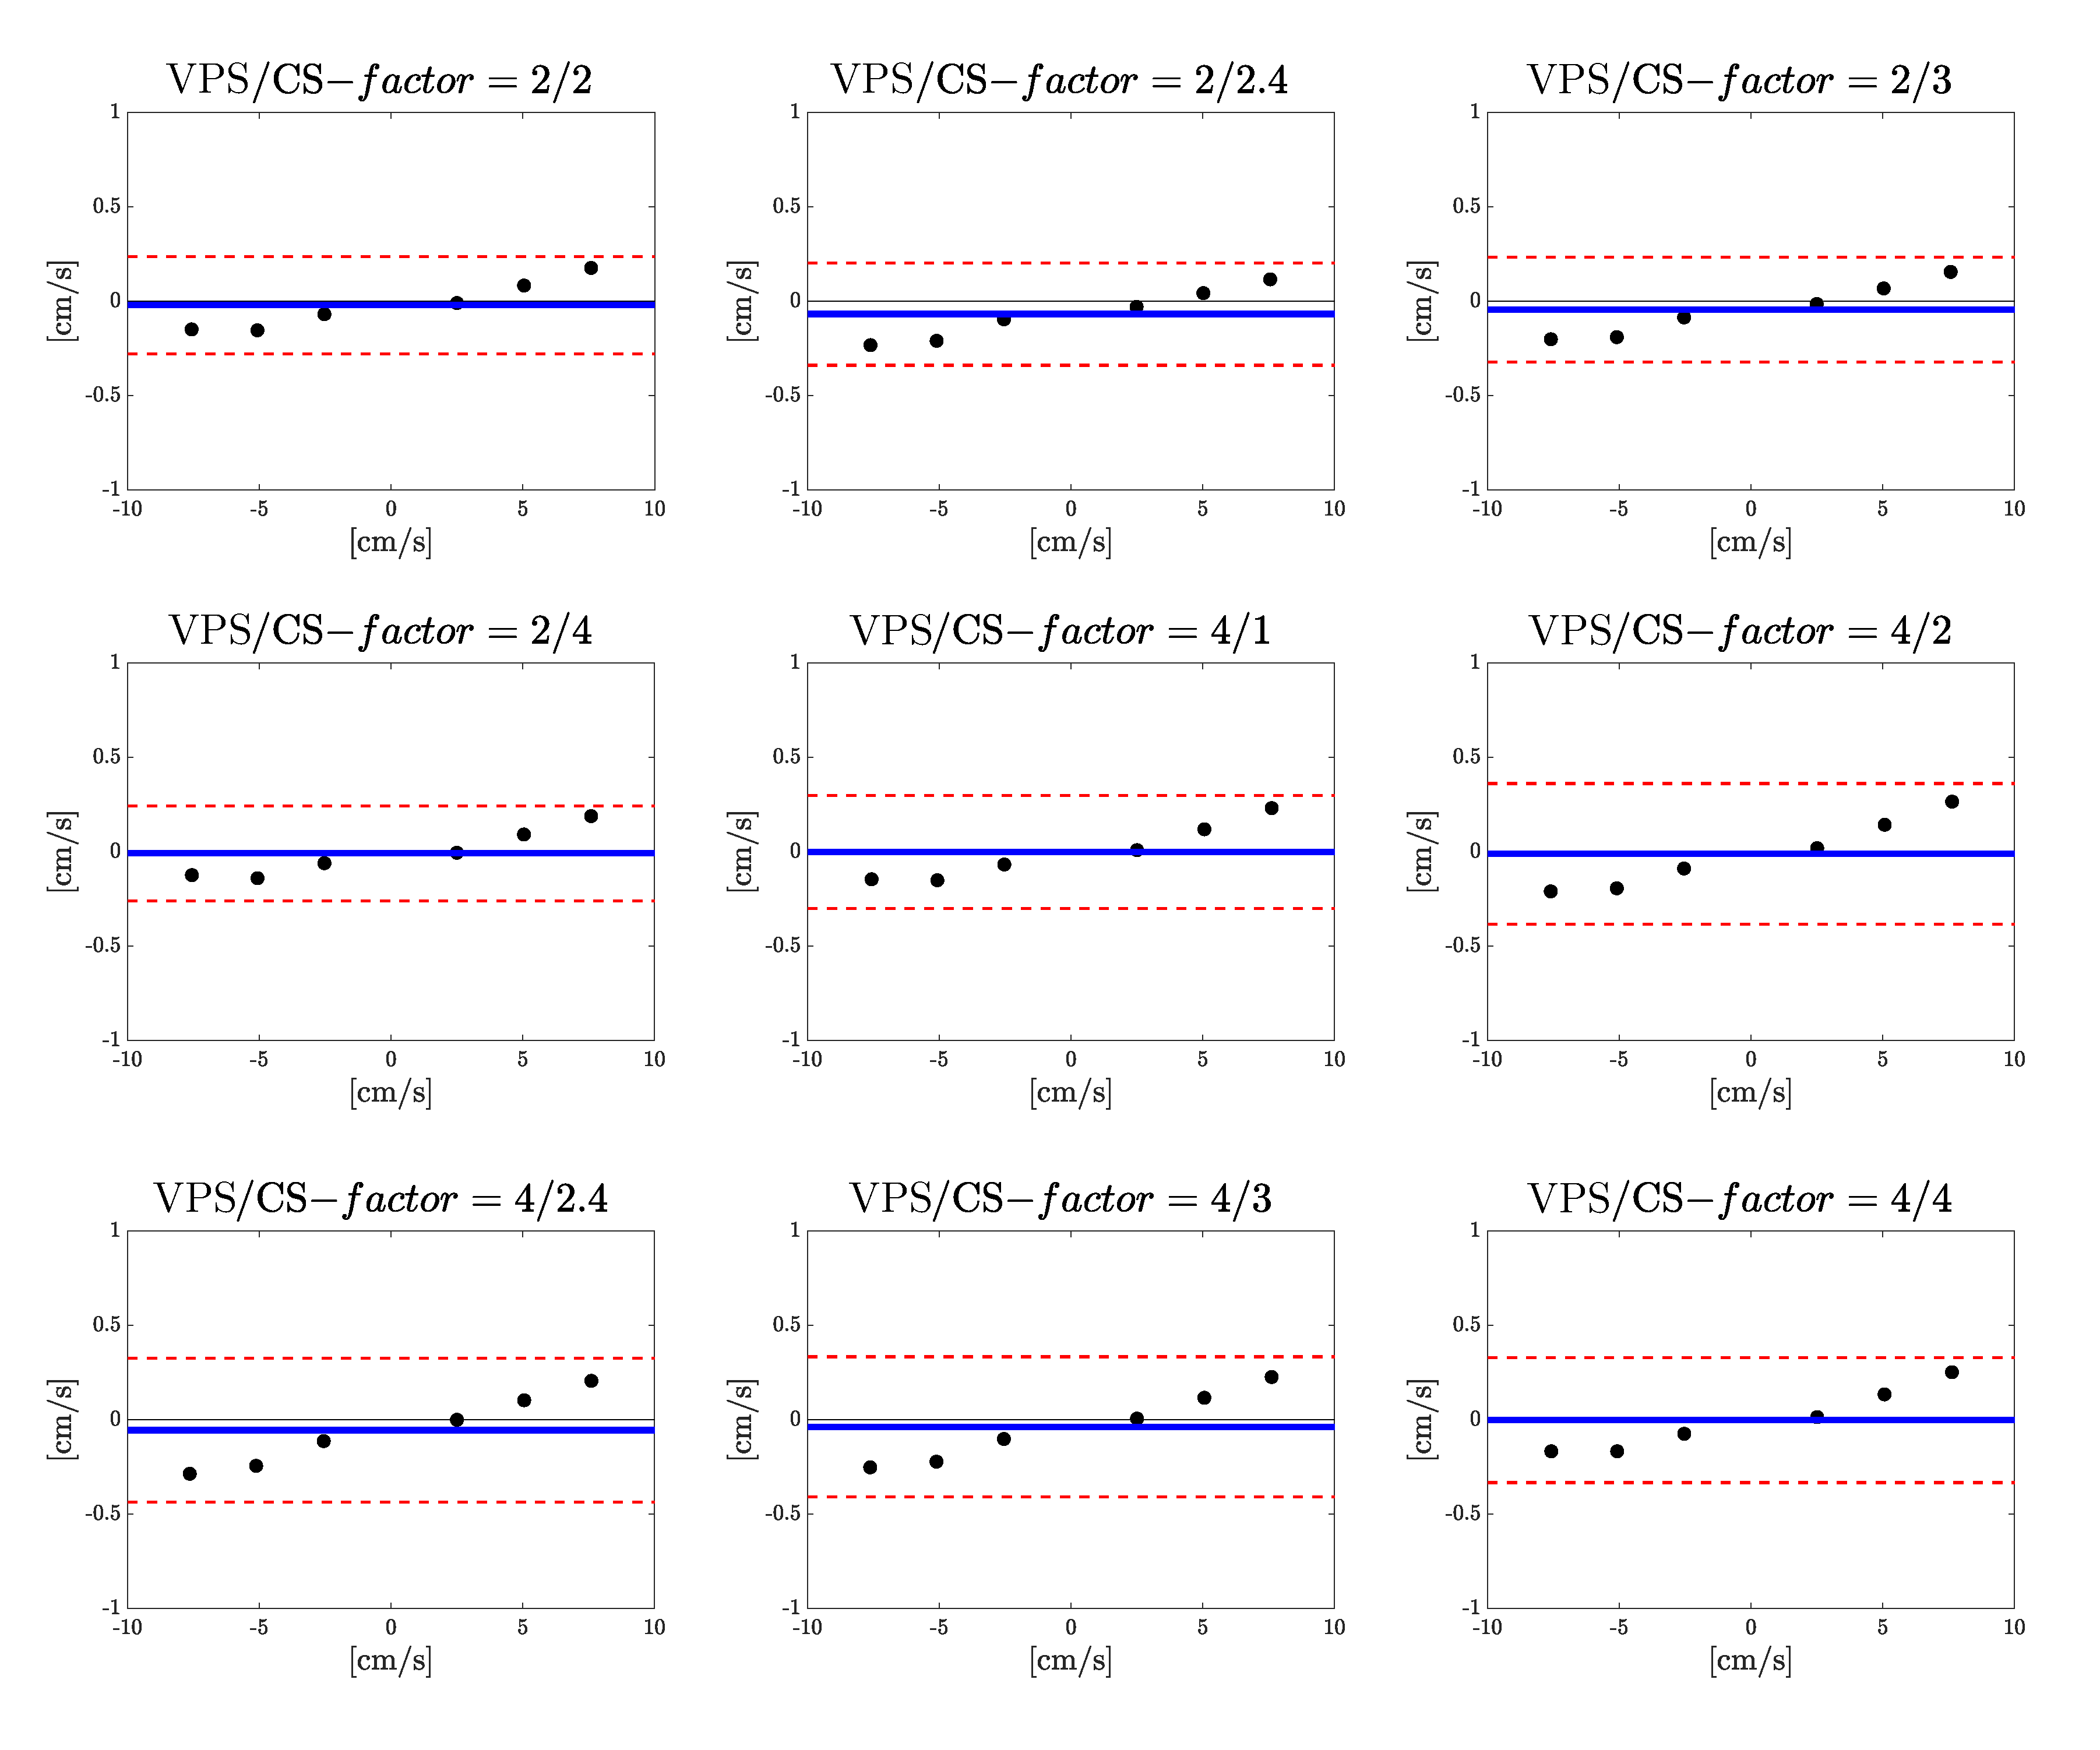
\includegraphics[width=\textwidth]{Figures/CS1_8.pdf}
\caption[Bland-Altman plots for velocity measurements for the constant flow phantom]{Bland-Altman plots for velocity measurements averaged in three regions of interest for the constant flow phantom for six different velocities. Measurements were performed for nine different combinations of views-per-segment (VPS) and undersampling factors (\mbox{CS\textit{-factor}}), flowmeter measurements are used as reference.}
\label{fig: CSS5}
\end{figure}
%*********************************************************
The agreement is high with the mean of the differences close to zero or with a small underestimation of $\SI{0.1}{\centi\meter/\second}$ for the different undersampled acquisitions compared to the flowmeter values. 
The 95\% confidence intervals across the different VPS/CS combinations range from $\pm \SI{0.25}{\centi\meter/\second}$ to $\pm \SI{0.4}{\centi\meter/\second}$. 
Notably, the mean difference of the velocities is dependent on the mean velocity; this dependency was attributed to the errors in the reference flowmeter velocity that increased with velocity. 
However, the \% difference between reference flowmeter and undersampled velocities was less than 2\% for any of the VPS/CS combinations. 
%-new paragraph-%

%-new paragraph-%
The optimization for the muscle data for the \mbox{CS\textit{-factor}} of 4 is shown in Figure~\ref{fig: CS5}. 
%*********************************************************
\begin{figure}[!hb]
\vspace{+0.2cm}
\centering
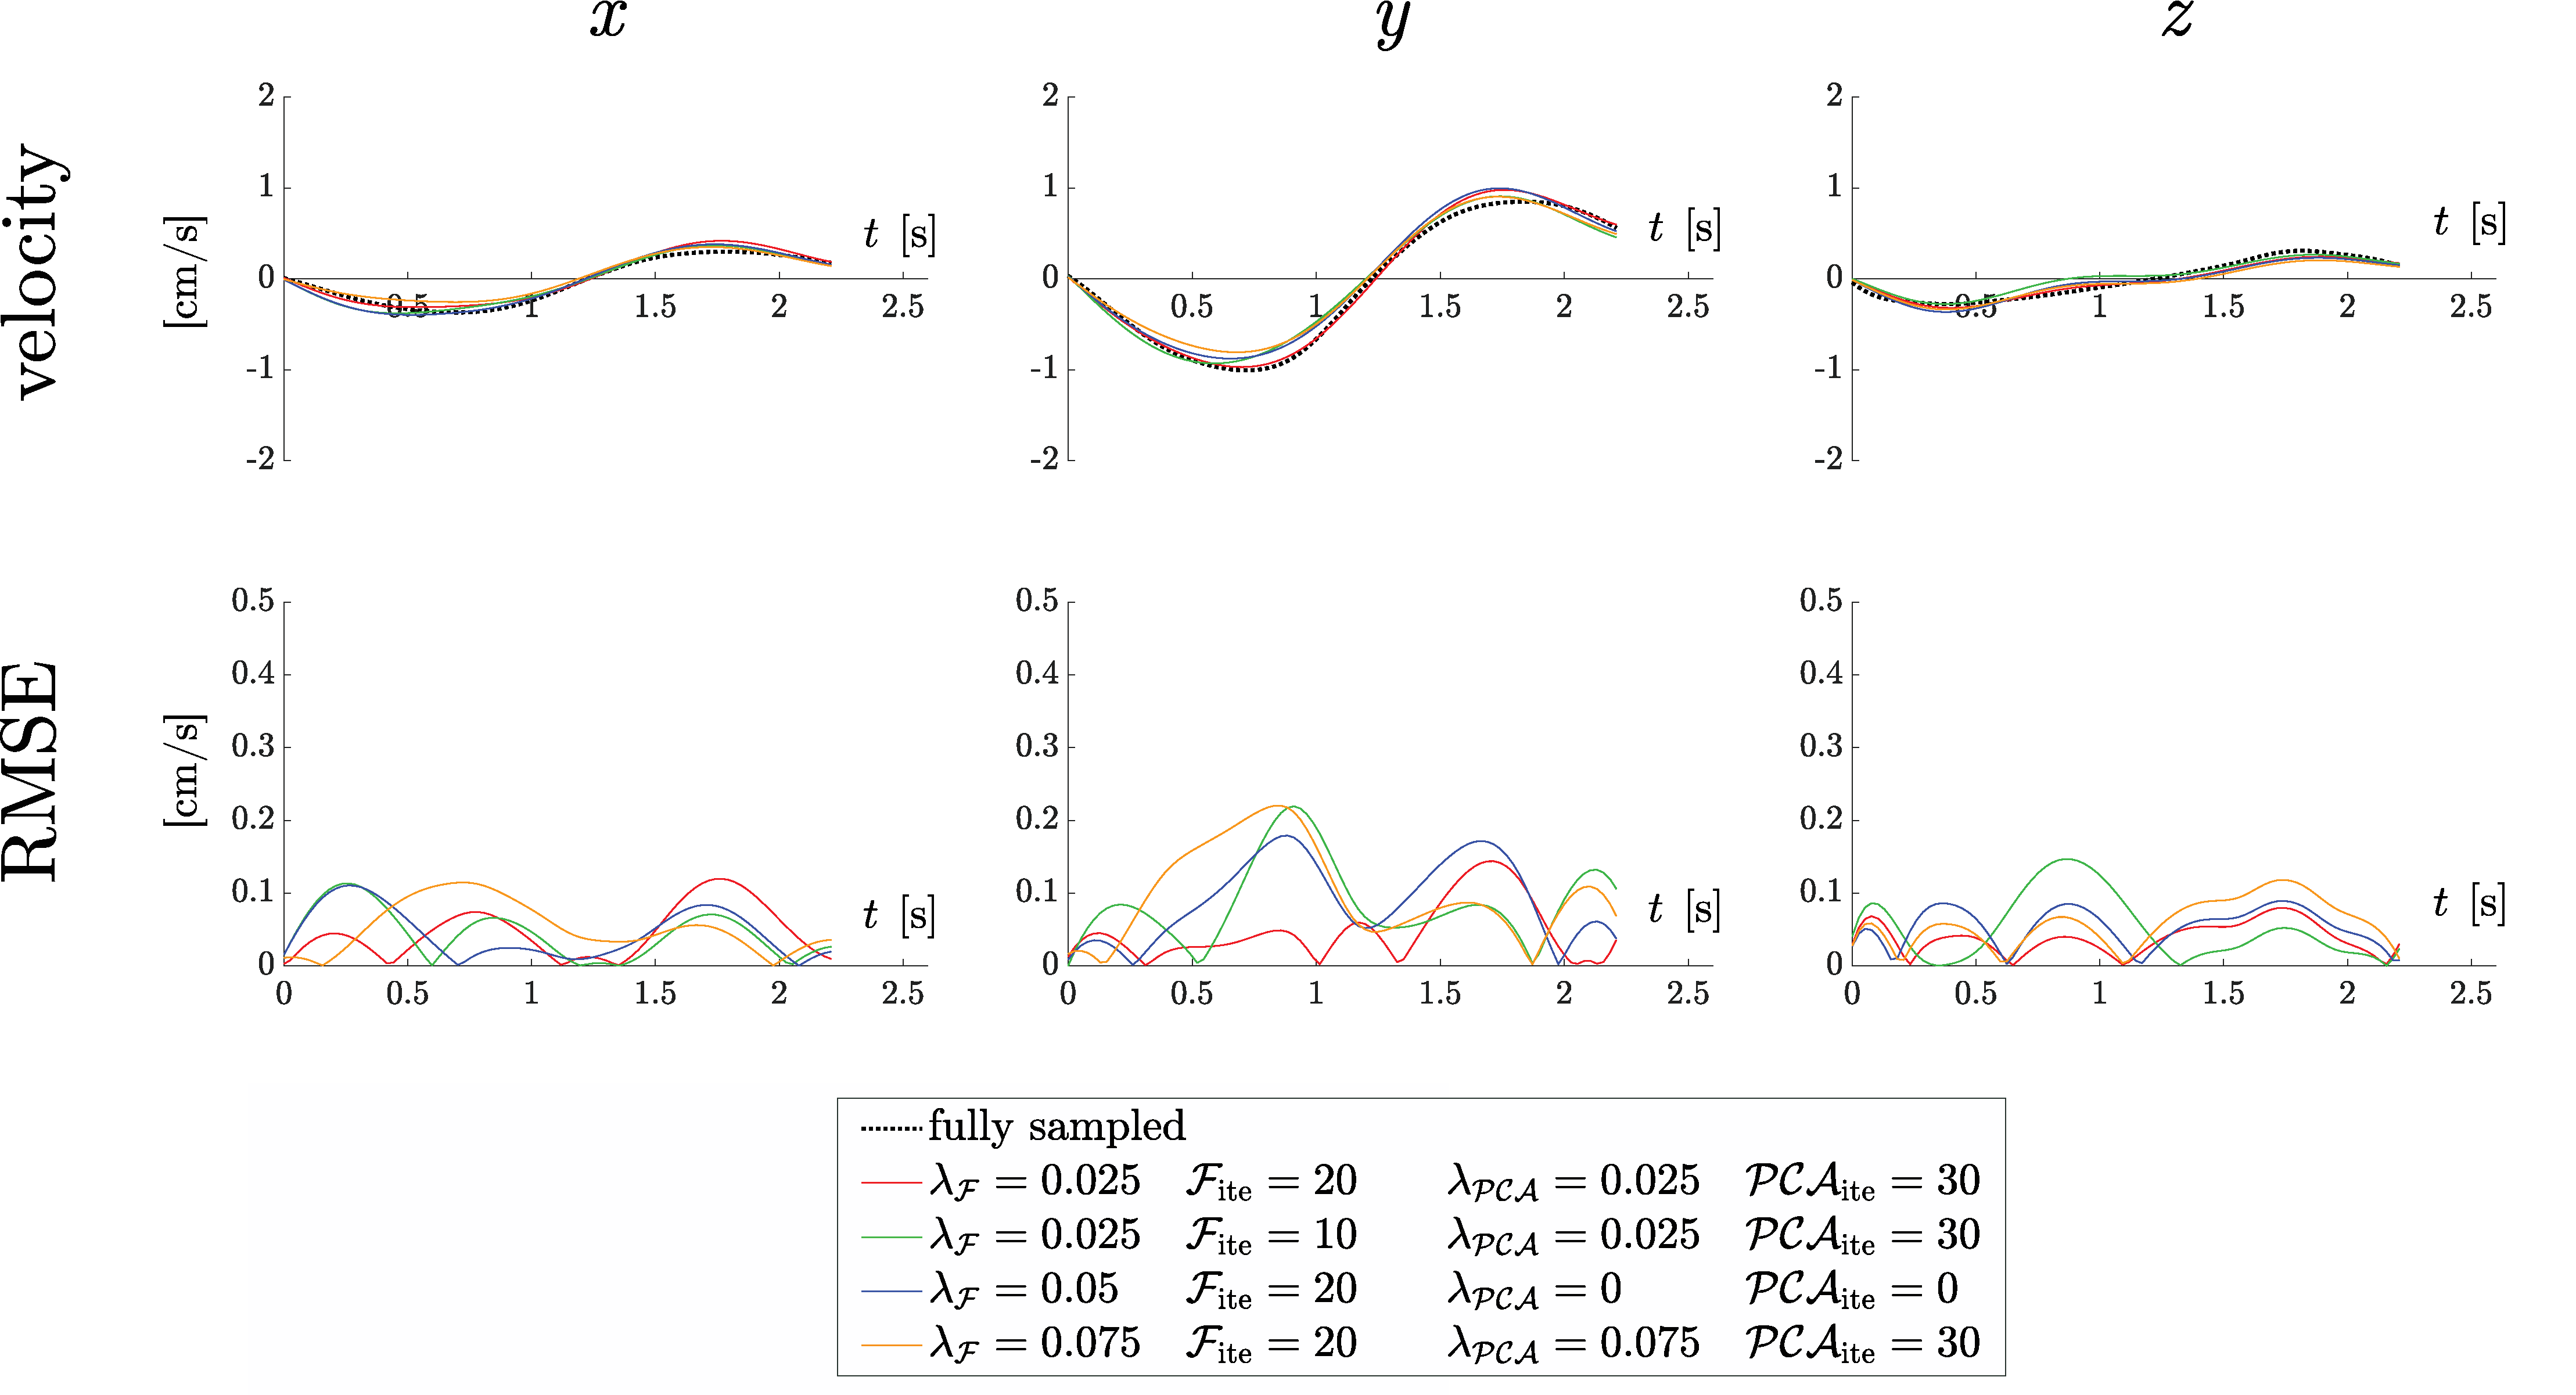
\includegraphics[width=\textwidth]{Figures/CS1_9.pdf}
\caption[Optimization of the compressed sensing parameters in human subject]{Optimization of the CS parameters in human subject. Each column represents each of the three orthogonal directions: $x$, $y$ (in-plane) and $z$ (out of plane). The plots of the velocities (top row), bottom row is the root-mean-squared error (RMSE) for each of the velocities. Plots with few best combinations only are shown here.}
\label{fig: CS5}
\end{figure}
%*********************************************************
The root-mean-square velocity at the peak of the contraction (in the large ROI placed in the MG) was used in calculating the RMSE for the optimization. 
Table~\ref{tab: CSS1} lists the regularization/iteration parameters for both steps of the reconstruction algorithm. 
%=========================================================
\begin{table}[!htb]
\vspace{+0.2cm}
\caption[Reconstruction parameters obtained for imaging sequences with different undersampling factors]{Reconstruction parameters obtained for imaging sequences with different undersampling factors.}
\label{tab: CSS1}
\begin{center}
\begin{tabular}{@{}ccccc@{}}
\toprule[1pt]\midrule[0.3pt]
\mbox{CS\textit{-factor}} & $\lambda_{\mathcal{F}}$ & $\mathcal{F}_{\mathrm{ite}}$ & $\lambda_\mathcal{PCA}$ & $\mathcal{PCA}_{\mathrm{ite}}$ \\ \midrule
4         & 0.025  & 20   & 0.025      & 30      \\
3         & 0.015  & 10   & 0.015      & 30      \\
2.4       & 0.010  & 10   & 0.010      & 20      \\
2         & 0.010  & 10   & 0          & 0       \\ \midrule[0.3pt]\bottomrule[1pt]
\end{tabular}
\end{center}
\vspace{-0.2cm}
\end{table}
%=========================================================
The value of ($\lambda_{\mathcal{F}/\mathcal{PCA}}$) and number of iterations decreased with the decrease in acceleration factors. 
Once the optimization was performed on one subject's muscle data, these parameters are used for the CS reconstruction of all \textit{in-vivo} data; the optimal parameters corresponding to each CS acceleration was chosen from Table~\ref{tab: CSS1}. 
%-new paragraph-%

%-new paragraph-%
Figure~\ref{fig: CS6} compares the phantom (static and flow) images acquired with the full \mbox{\textit{k-}space}, simulated and actual undersampled data acquired with \mbox{CS\textit{-factor}} of 4 at select temporal frames. 
%*********************************************************
\begin{figure}[!htb]
\vspace{+0.2cm}
\centering
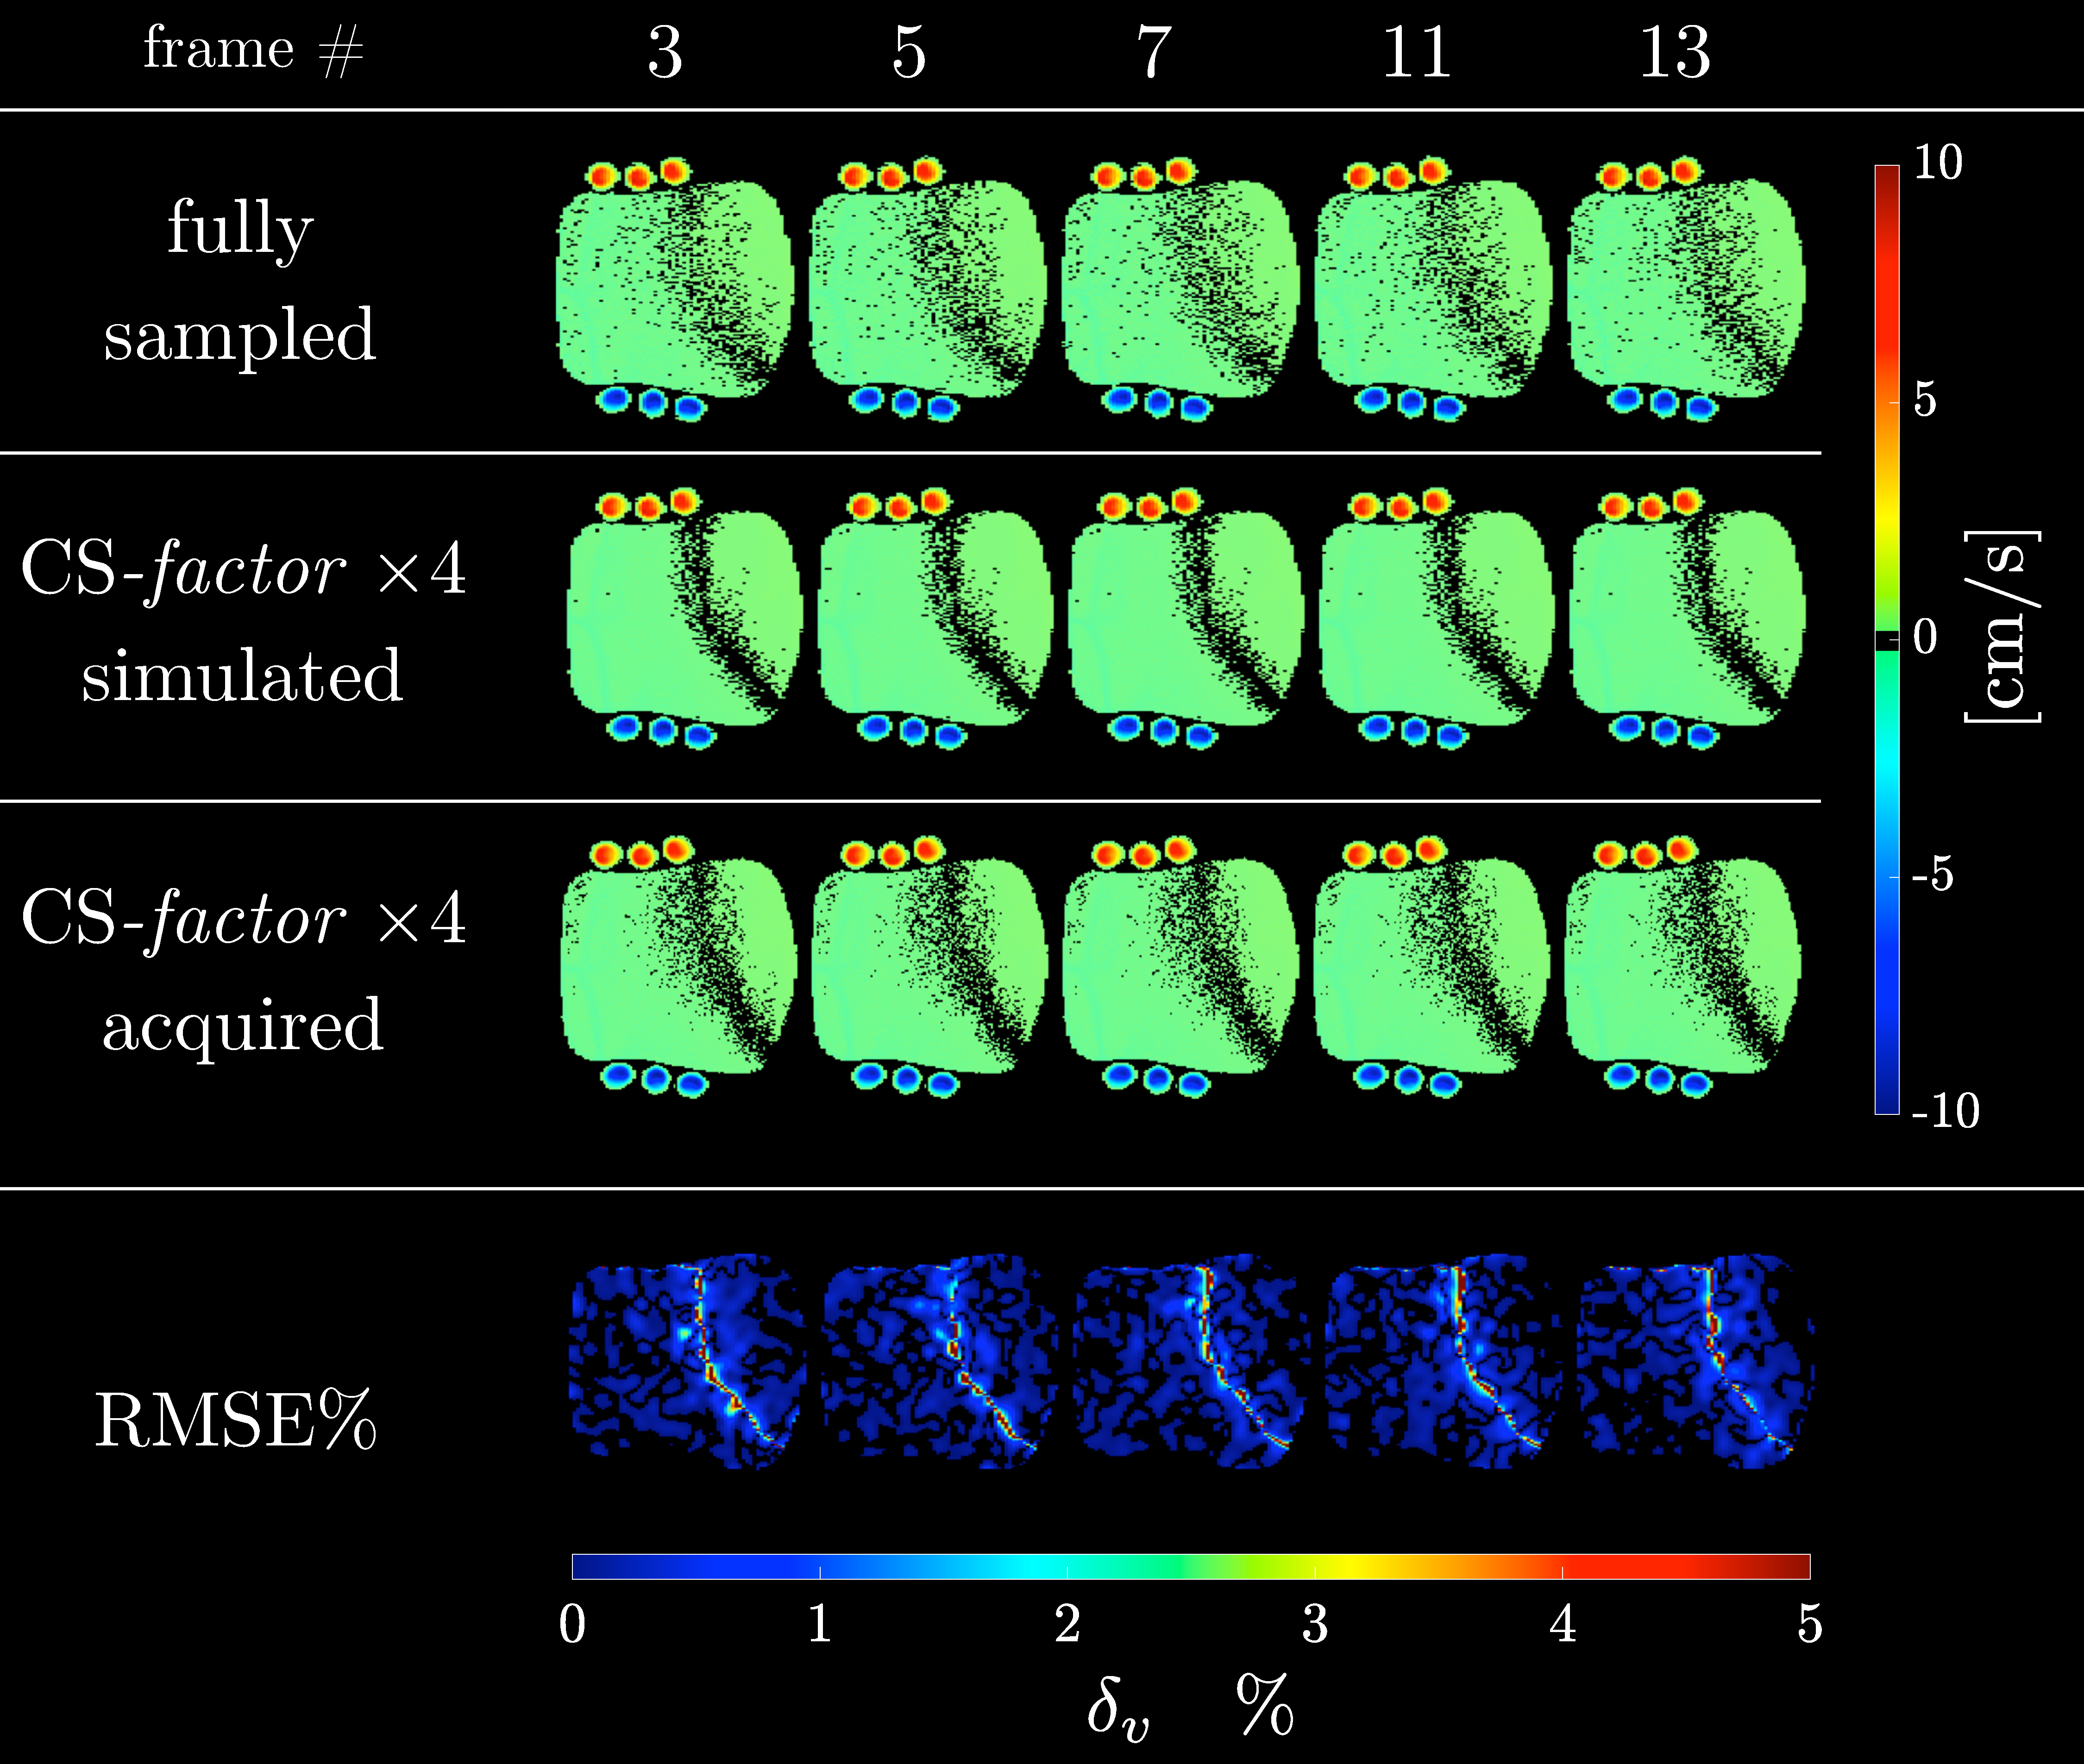
\includegraphics[width=0.9\textwidth]{Figures/CS1_10.pdf}
\caption[Velocity colormaps of the constant flow phantom at five temporal frames]{Velocity colormaps of the constant flow phantom at five temporal frames. The first row (fully sampled) velocity data, simulated undersapmpled (second row) and the acquired undersampled (third row) velocity data. RMSE maps of the difference in velocities of images in the first and third rows (last row).}
\label{fig: CS6}
\end{figure}
%*********************************************************
In the undersampled images, the static phantom is mapped correctly to values close to zero velocity (green shade in the color map) while flow out of the imaging plane is in red shade and into the imaging plane is in blue shade. 
The visual similarity of the fully sampled and undersampled velocity images is clearly evident. 
This is also confirmed by the root mean square error map of the fully sampled and acquired undersampled images shown in the last row. 
The flow phantoms are not visible on the RMSE maps (showing very close agreement between the velocities from full \mbox{\textit{k-}space} and undersampled \mbox{\textit{k-}space}) and there is only the background static phantom with very small RMSE errors. 
%-new paragraph-%

%-new paragraph-%
Figure~\ref{fig: CSS6} shows simulated muscle data from random undersampling (CS factors of 4 and 6) and the resultant magnitude images after CS reconstruction.
%*********************************************************
\begin{figure}[!htb]
\vspace{+0.2cm}
\centering
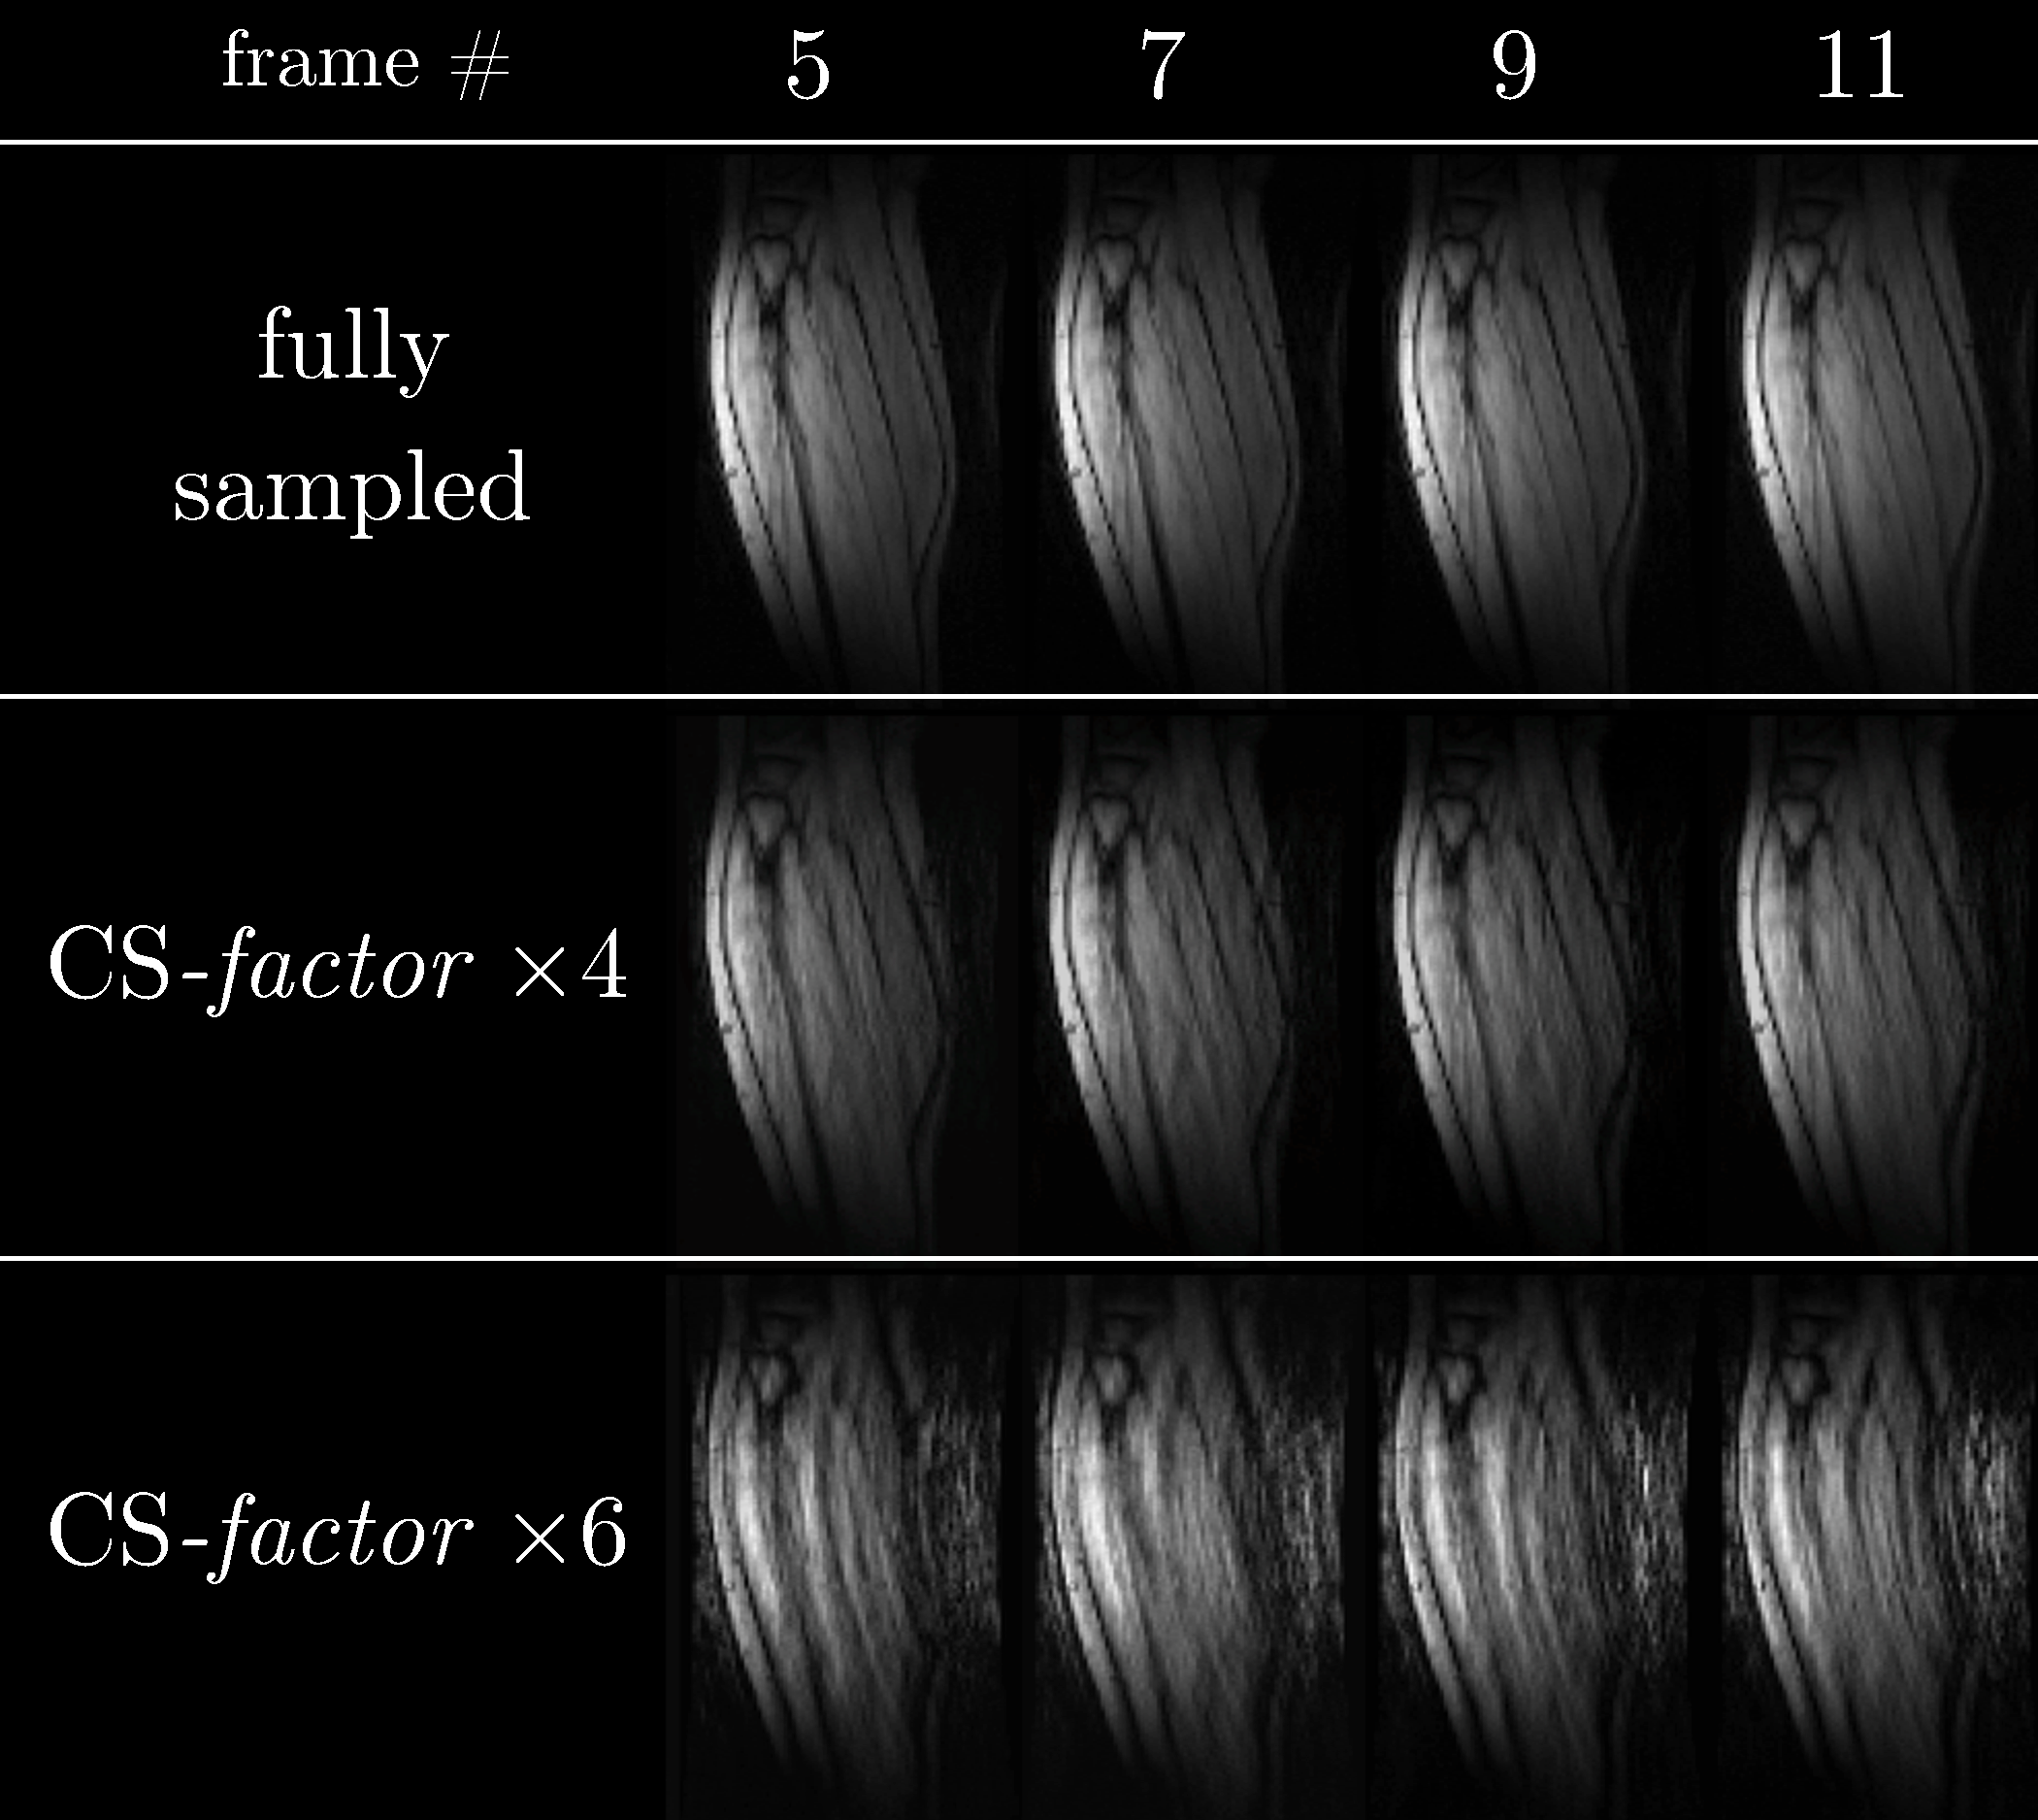
\includegraphics[width=0.9\textwidth]{Figures/CS1_11.pdf}
\caption[Selected frames of magnitude images reconstructed from the fully-sampled, undersampled \mbox{\textit{k-}space} with factors 4 and 6]{Selected frames of magnitude images reconstructed from the fully-sampled \mbox{\textit{k-}space} (top row), undersampled \mbox{\textit{k-}space} with factors 4 (middle row) and 6 (bottom row).}
\label{fig: CSS6}
\end{figure}
%********************************************************* 
The presence of artifacts at CS factor of 6 is visually evident. 
Color coded muscle velocity images of the fully sampled and the acquired undersampled images are shown in Figure~\ref{fig: CS7} as a function of the isometric contraction cycle for 17 temporal frames.
These are oblique sagittal images positioned to obtain the fibers of the medial gastrocnemius (MG) in the plane of the image. 
The two stage CS reconstruction using the optimized parameters based on muscle velocity images resulted in undersampled images that were visually close to the images reconstructed from fully sampled \mbox{\textit{k-}space} data. 
The spatial and temporal patterns of velocity are very similar for the full \mbox{\textit{k-}space} and the undersampled acquisitions.
%*********************************************************
\begin{sidewaysfigure}
\vspace{+0.2cm}
\centering
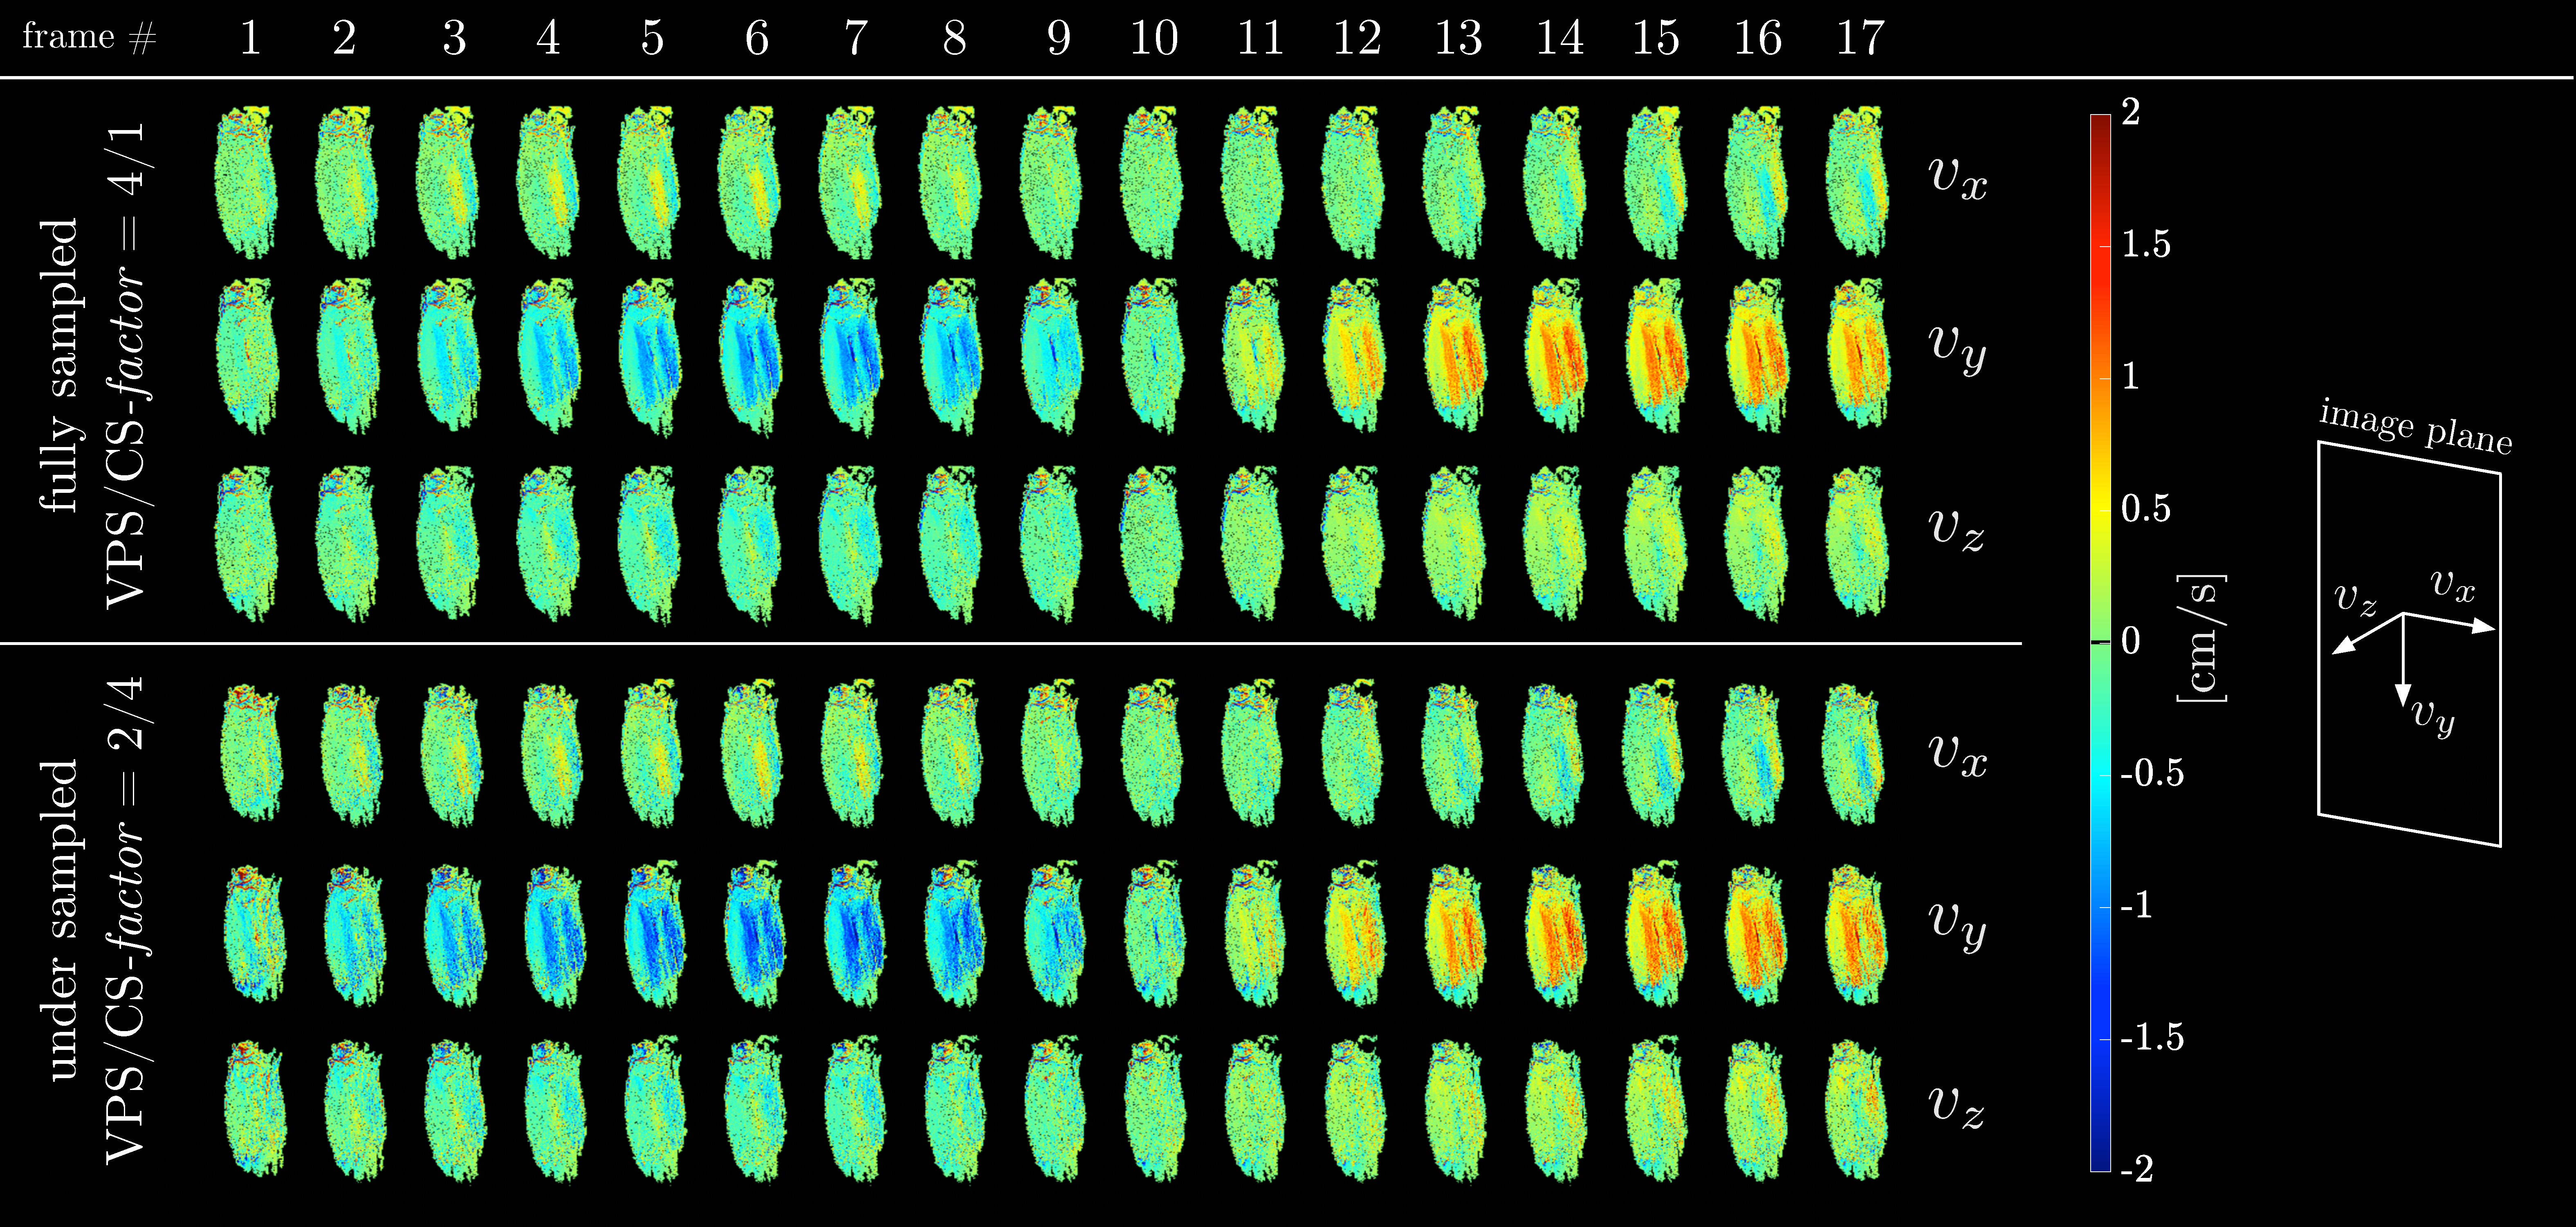
\includegraphics[width=8.5in]{Figures/CS1_12.pdf}
\captionsetup{width=8.5in}
\caption[Velocity colormaps for all three orthogonal directions in the oblique sagittal section through the calf muscles]{Velocity colormaps for all three orthogonal directions in the oblique sagittal section through the calf muscles; The fully sampled (top section) followed by undersampled (by a factor of $\times 4$) reconstructed using the parameters obtained through the optimization process.}
\label{fig: CS7}
\end{sidewaysfigure}
%*********************************************************  
The velocity in the image $y$-axis is the highest as this corresponds to the superior to inferior (SI) direction and the lowest velocity is in the $z$-direction which maps the out-of-plane motion. 
The blue shades are negative velocities around the peak of the isometric contraction (temporal frames 4 to 8) and the red shades are positive velocities at the peak of the relaxation (temporal frames 12 to 16).
Figure~\ref{fig: CS8} is a plot of the $v_y$ velocity component (averaged over the eleven subjects) as a function of the dynamic cycle measured in ROIs placed in the MG extracted from the full \mbox{\textit{k-}space} as well as from the undersampled \mbox{\textit{k-}space} with the different CS and VPS factors.
%*********************************************************
\begin{figure}[!htb]
\vspace{+0.2cm}
\centering
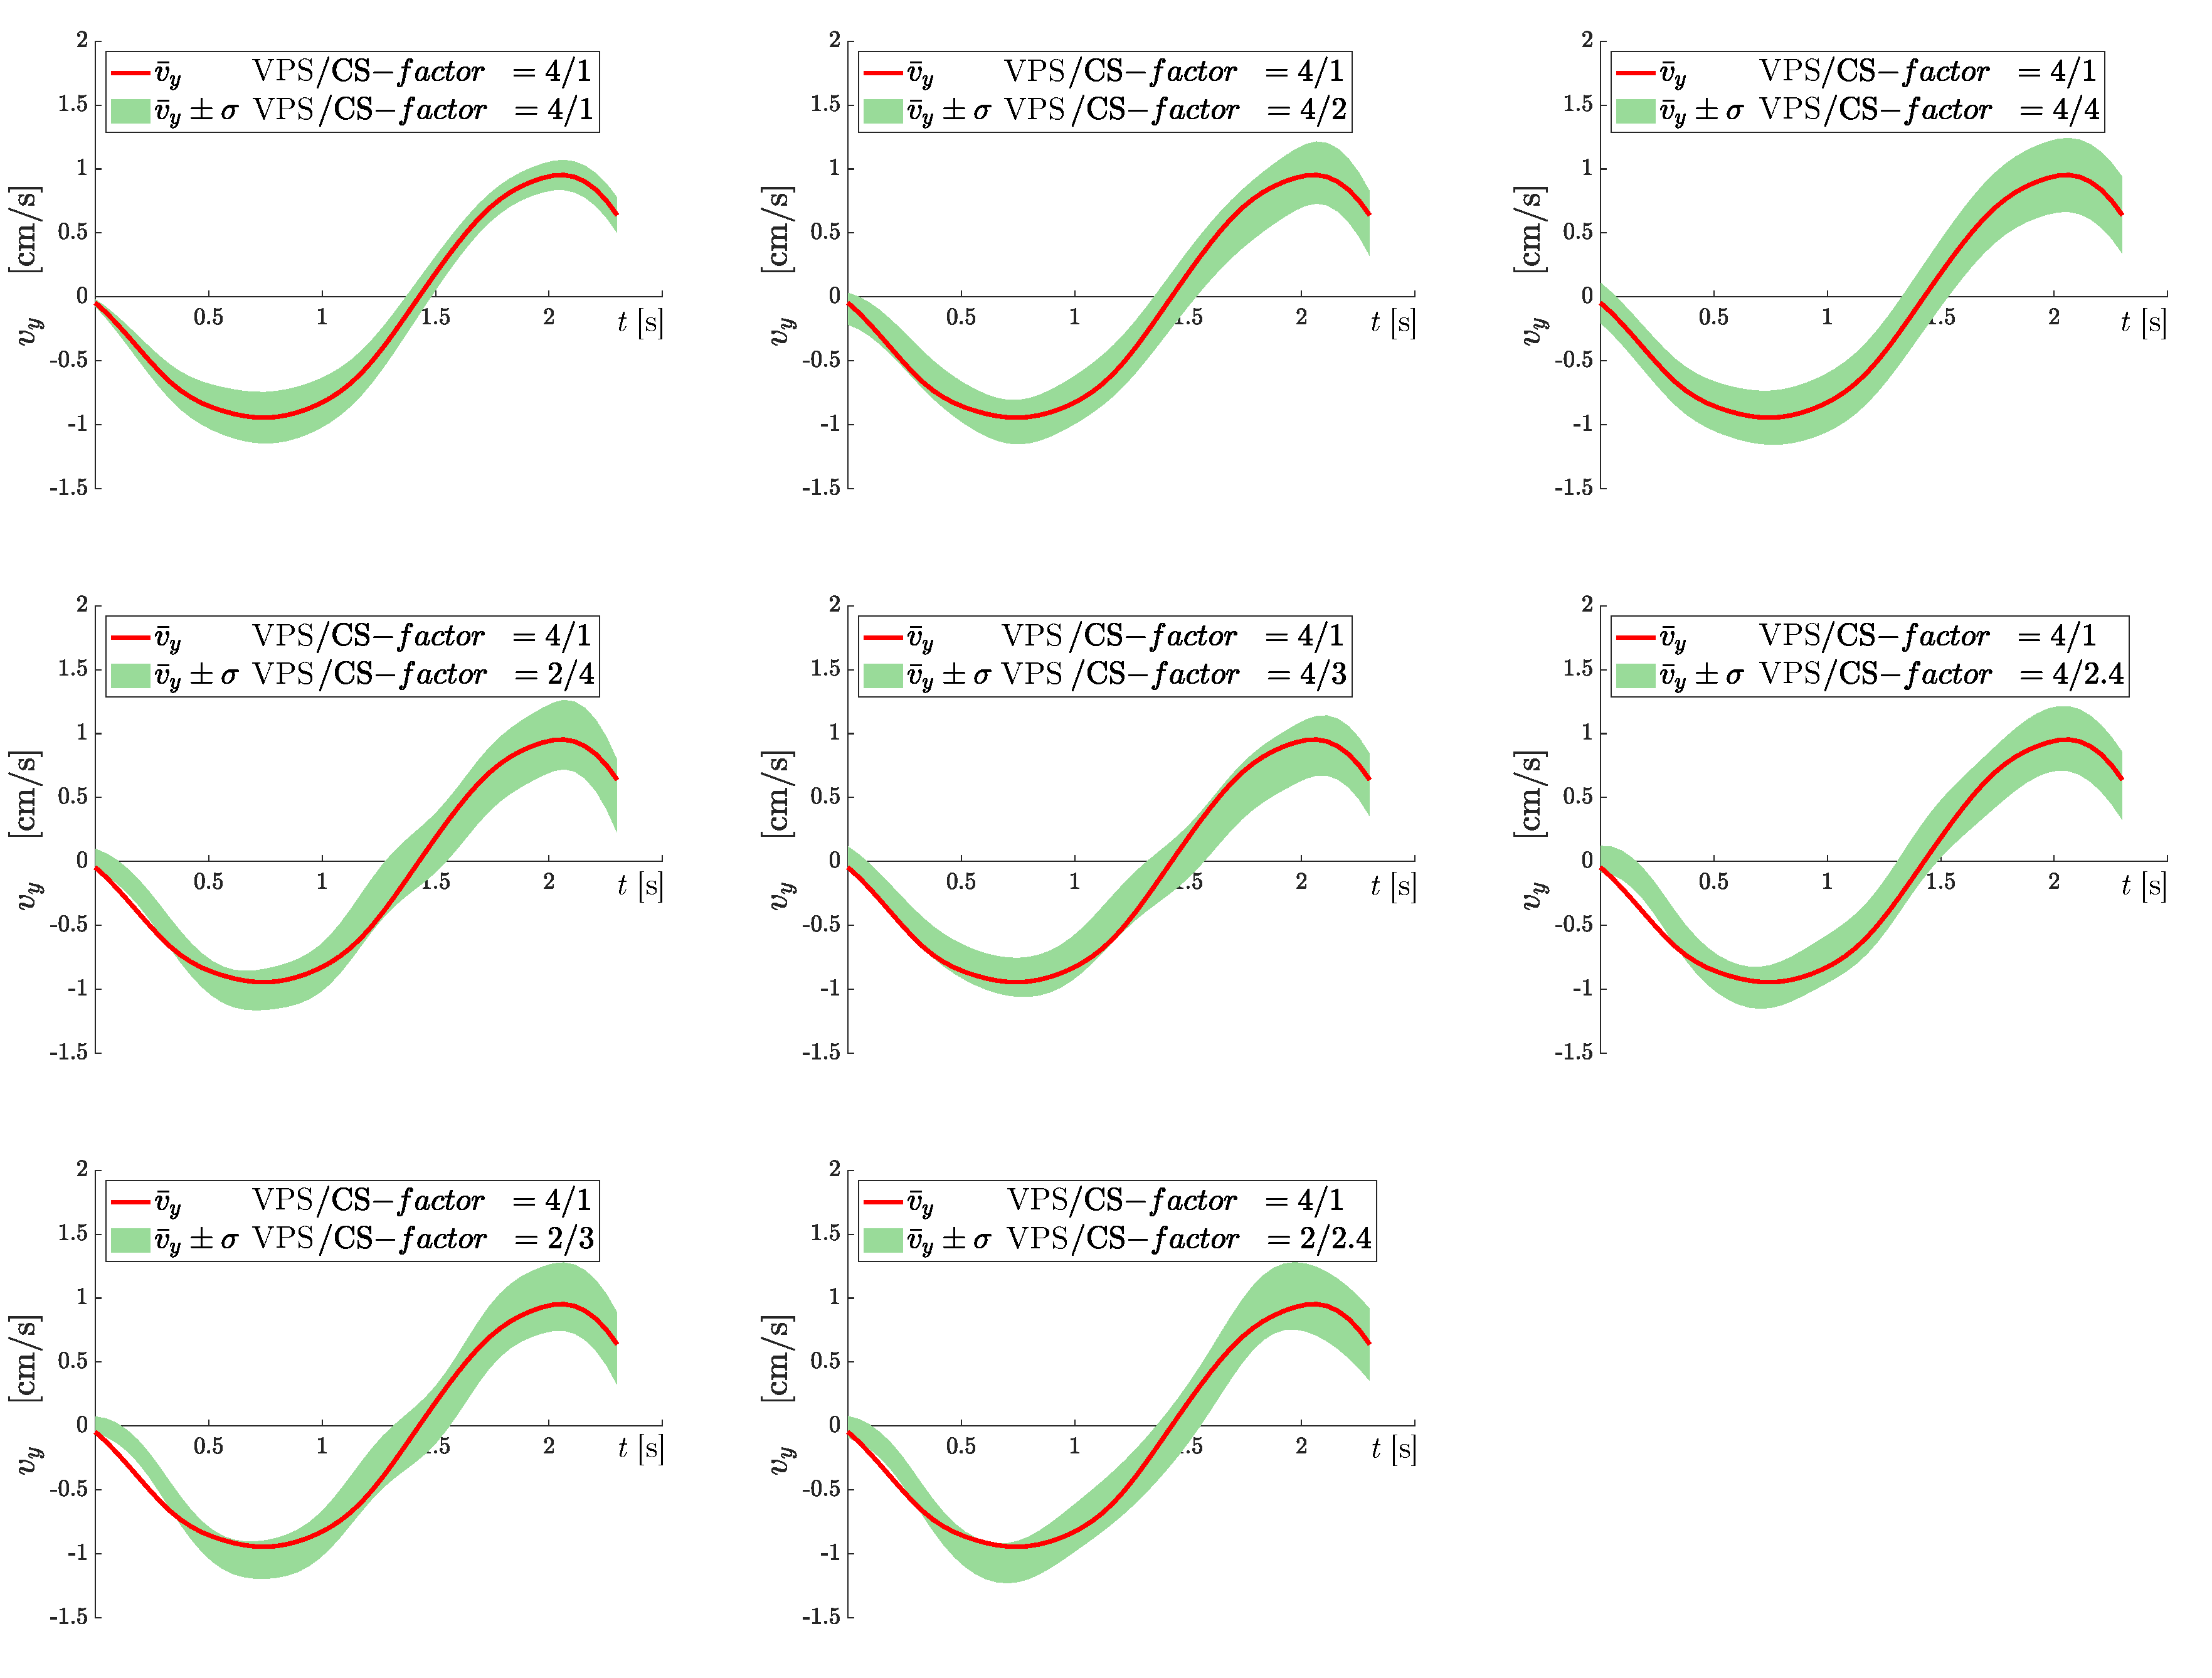
\includegraphics[width=\textwidth]{Figures/CS1_13.pdf}
\caption[Velocity $v_y$ plots as a function of the isometric contraction for scans acquired with 8 different VPS/\mbox{CS\textit{-factor}}]{Velocity $v_y$ plots as a function of the isometric contraction for scans acquired with 8 different VPS/\mbox{CS\textit{-factor}}. The values are the mean over the eleven subjects, the green shaded region reflects mean $\pm$ standard deviation. The red line is the mean (average of subjects) for the full \mbox{\textit{k-}space} acquisition.}
\label{fig: CS8}
\end{figure}
%********************************************************* 
The good agreement between the $v_y$ values from the reference and undersampled acquisitions is confirmed by the overlay of the mean $v_y$ from full \mbox{\textit{k-}space} on the $v_y \pm \sigma$ (average over 11 subjects) from the undersampled acquisitions. 
%-new paragraph-%

%-new paragraph-%
One of the goals of velocity mapping is to derive the strain or strain rate tensor to study muscle kinematics. 
It is important to note that both strain and strain rate are sensitive to noise as spatial gradients are calculated from the velocity or displacement maps to extract strain/strain rate; the use of the anisotropic diffusion filter to denoise was critical to the calculation of the strain rate maps (Figure~\ref{fig: CSS3}). 
Figure~\ref{fig: CS9} shows strain rate images (absolute values at the peak value in the contraction phase) calculated from the velocity maps acquired with different combinations of CS and VPS factors; SR image quality is maintained at the highest acceleration factors. 
%*********************************************************
\begin{figure}[!htb]
\vspace{+0.2cm}
\centering
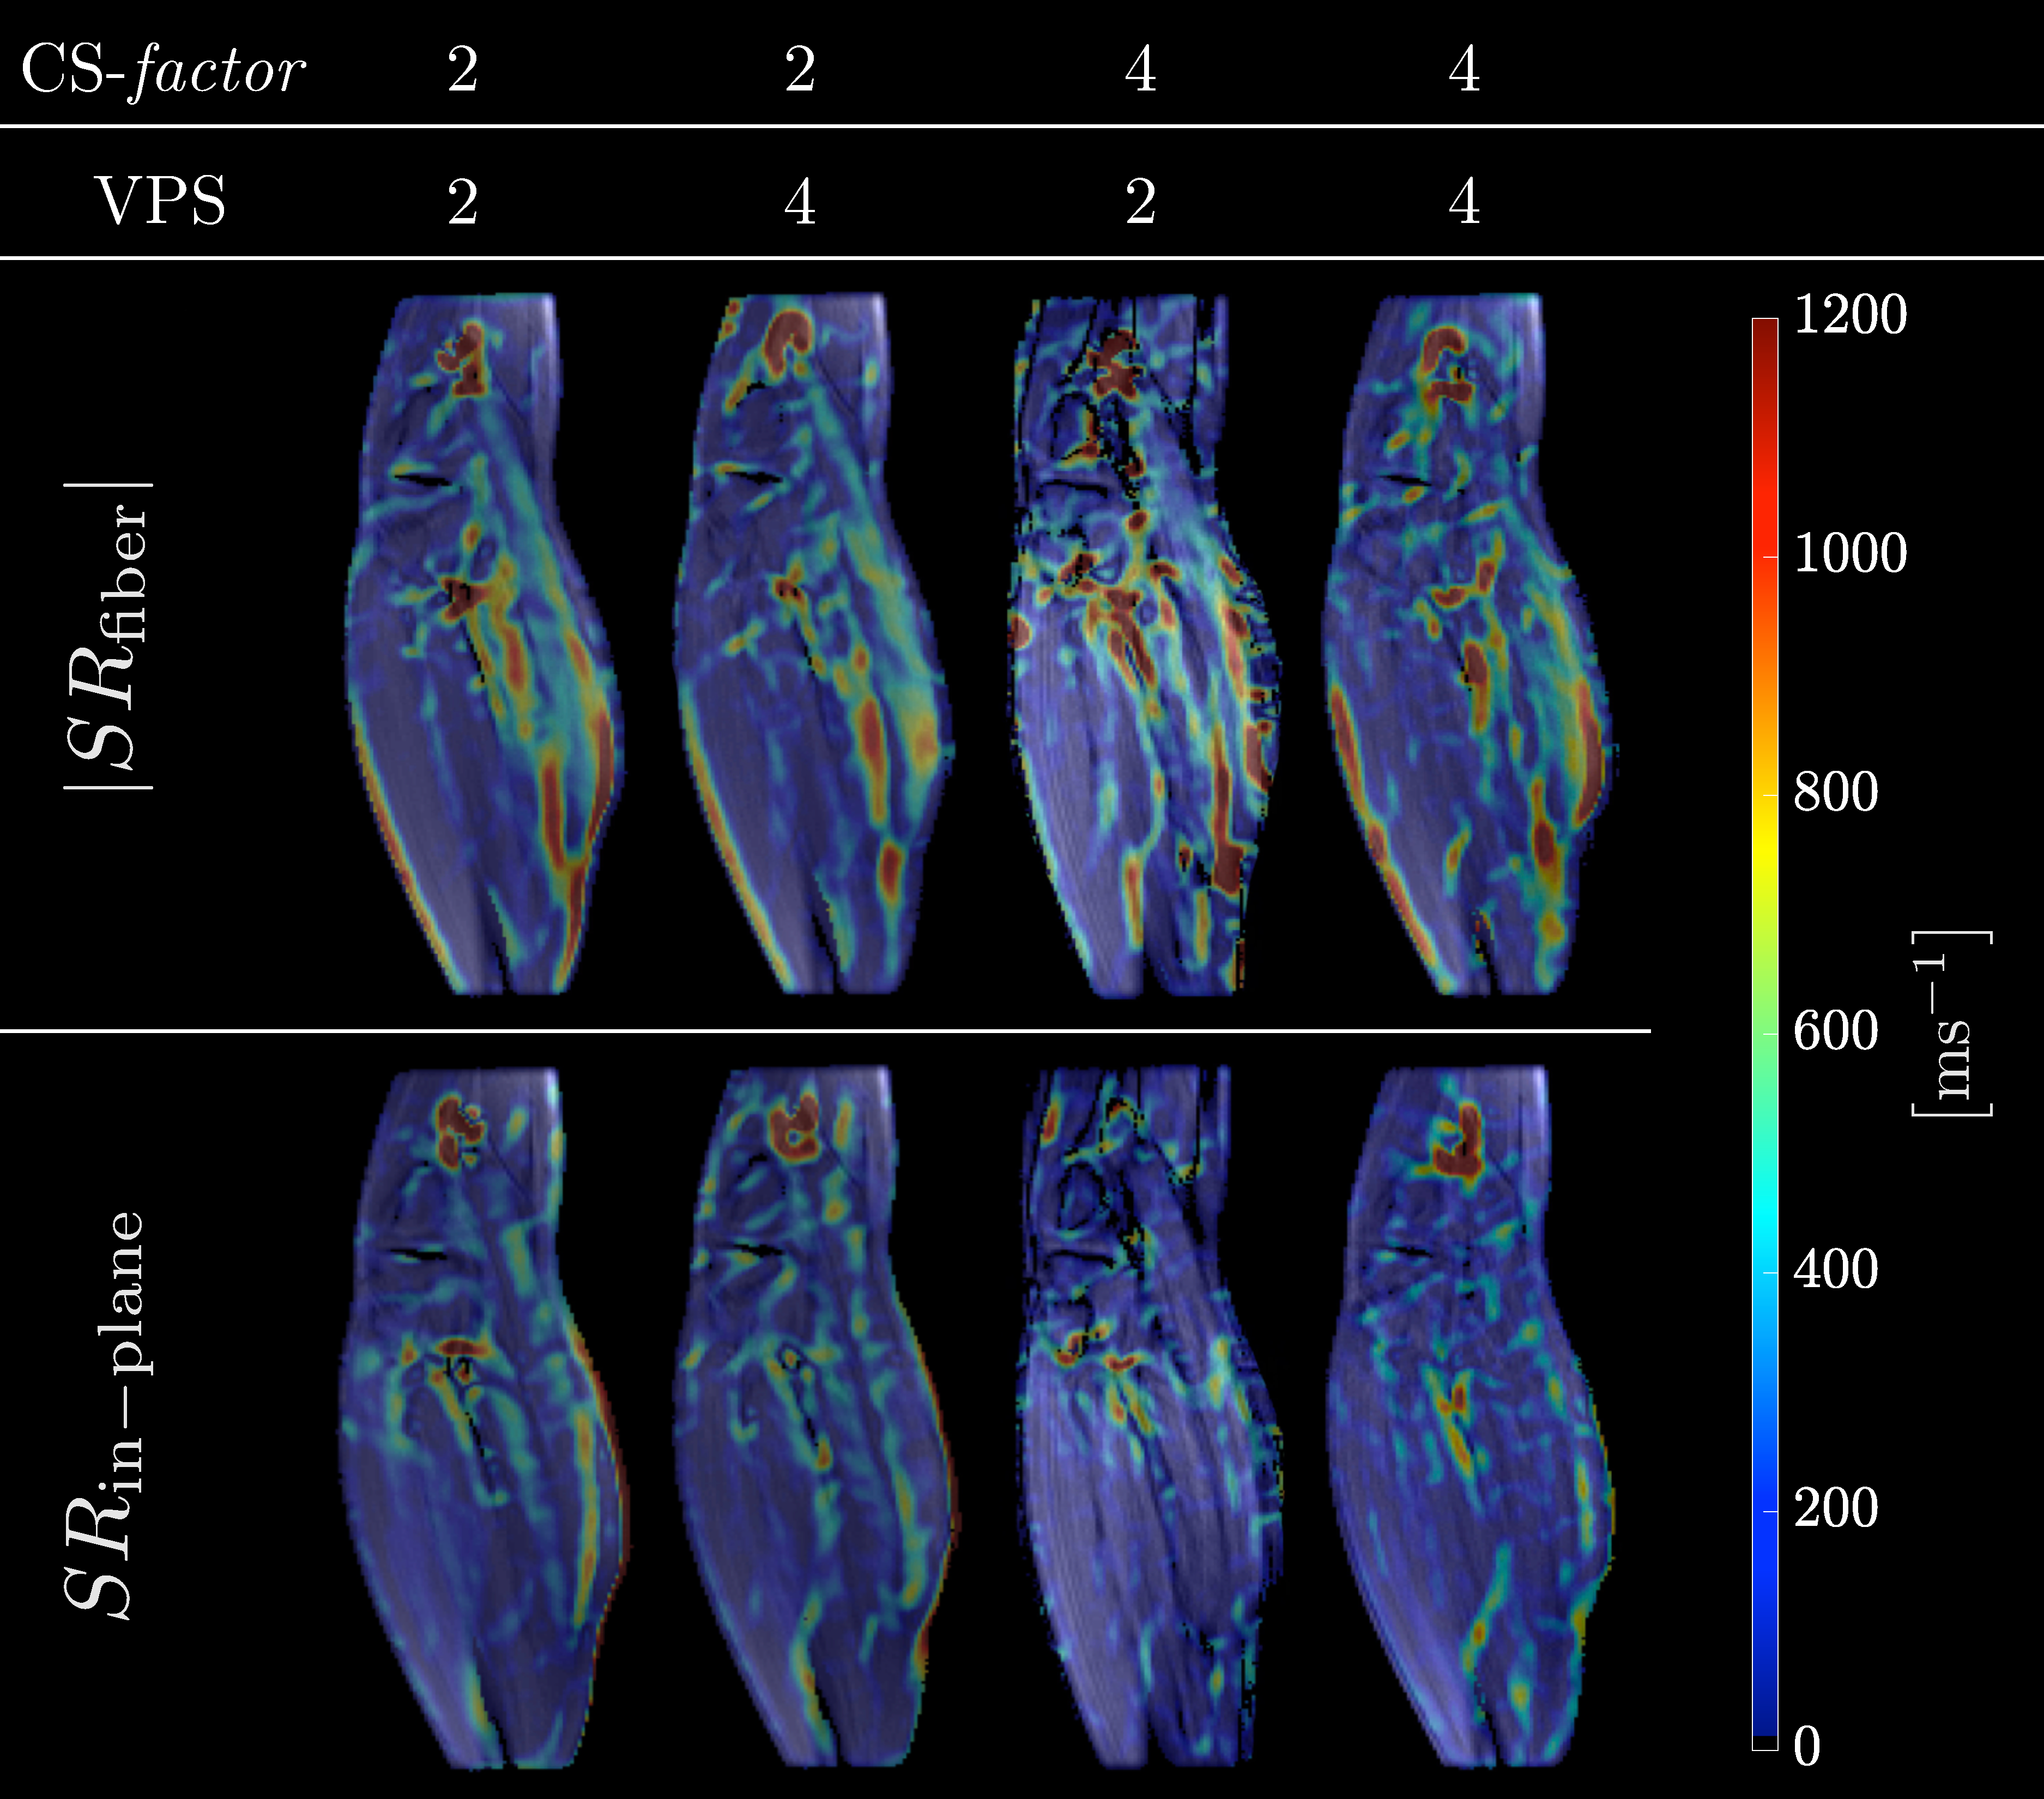
\includegraphics[width=0.9\textwidth]{Figures/CS1_14.pdf}
\caption[Absolute value strain rate tensor eigenvalue colormaps derived from velocity images for 4 different combinations of VPS/\mbox{CS\textit{-factor}}]{Absolute value strain rate tensor eigenvalue colormaps derived from velocity images for 4 different combinations of VPS/\mbox{CS\textit{-factor}}. The $SR_\mathrm{fiber}$ and $SR_\mathrm{in-plane}$ correspond to the strain rate maps along and perpendicular to the fiber direction respectively; shown here is one temporal frame at the peak of the contraction phase.}
\label{fig: CS9}
\end{figure}
%********************************************************* 
Bland-Altman plots (Figure~\ref{fig: CS10}) and the indices extracted from these plots (Table~\ref{tab: CS2}) show good agreement between the full \mbox{\textit{k-}space} acquisition and the subsampled acquisitions (average of mean differences ranges from 0.5\% to 6.7\% across the VPS/\mbox{CS\textit{-factor}} combinations).
%*********************************************************
\begin{figure}[!htb]
\vspace{+0.2cm}
\centering
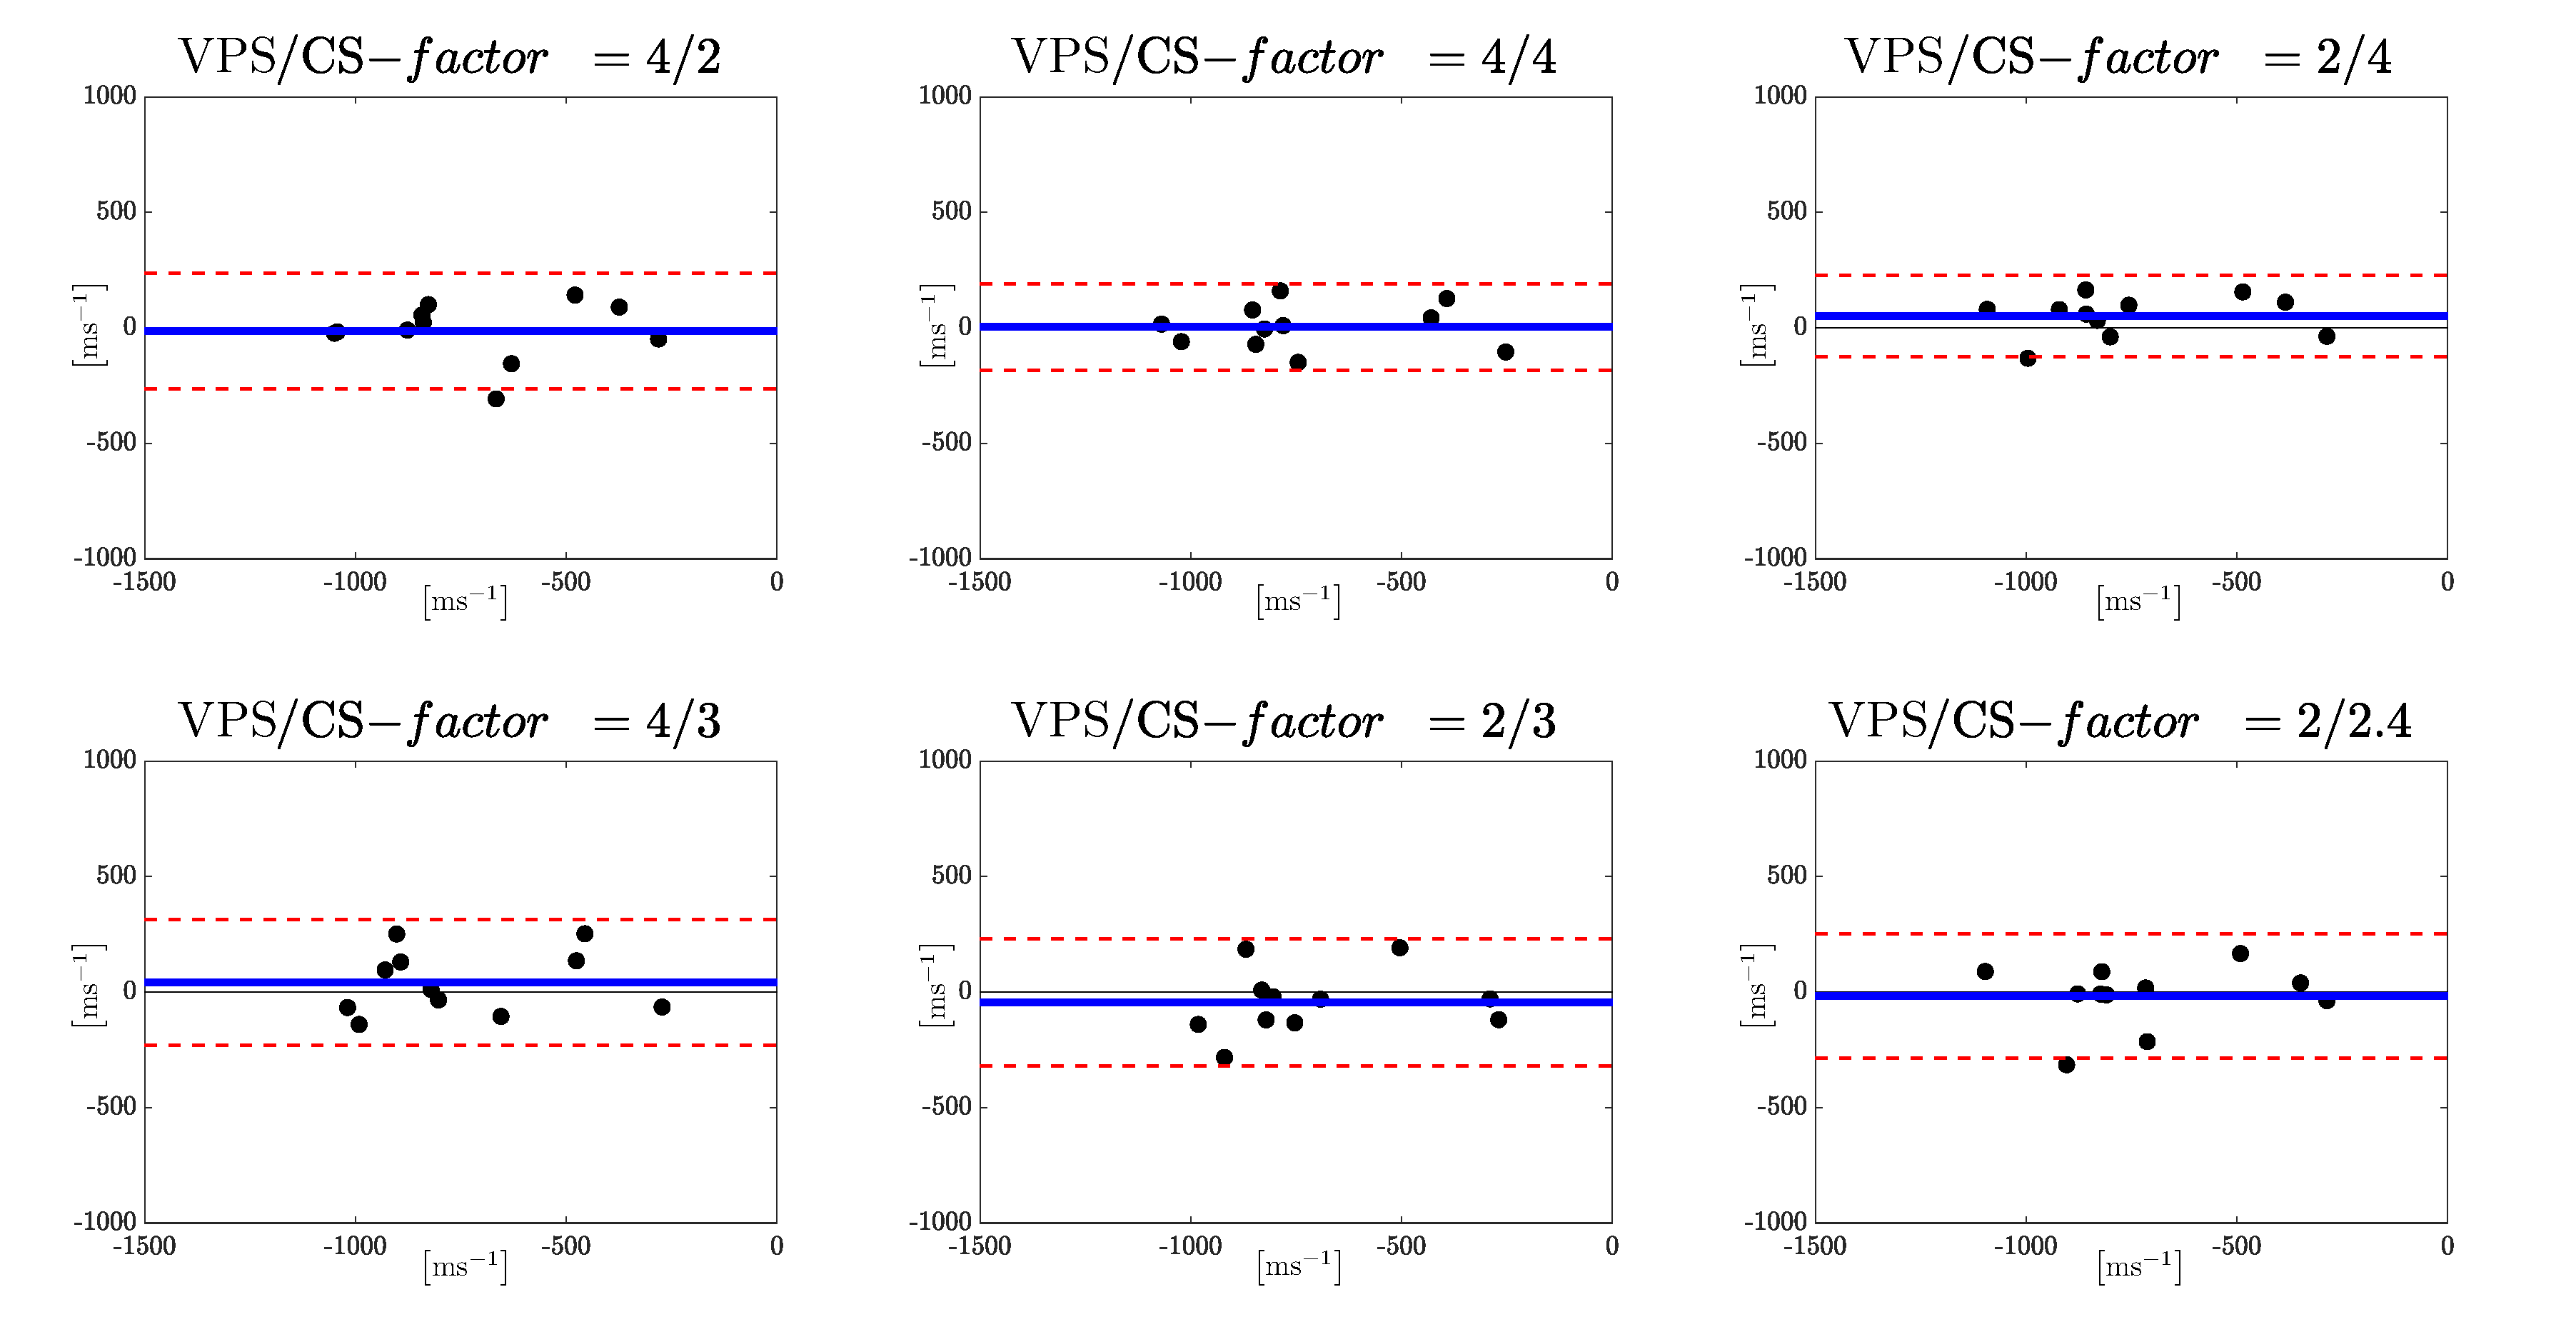
\includegraphics[width=\textwidth]{Figures/CS1_15.pdf}
\caption[Bland-Altman plots for the peak $SR_\mathrm{fiber}$ values during the contraction part of the cycle for 6 different combinations of VPS/\mbox{CS\textit{-factor}}]{Bland-Altman plots for the peak $SR_\mathrm{fiber}$ values during the contraction part of the cycle for 6 different combinations of VPS/\mbox{CS\textit{-factor}}. Mean value between fully sampled and undersampled data is shown in blue, the 95\% confidence interval is shown in dotted red lines.}
\label{fig: CS10}
\end{figure}
%********************************************************* 
%=========================================================
\begin{table}[!htb]
\vspace{+0.2cm}
\caption[Parameters obtained from the Bland-Altman plots of peak strain rates for seven different combinations of views per segment and undersampling factors]{Parameters obtained from the Bland-Altman plots (Figure~\ref{fig: CS10}) of peak strain rates for seven different combinations of views per segment (VPS) and undersampling factors (\mbox{CS\textit{-factor}}).}
\label{tab: CS2}
\begin{center}
\begin{tabular}{@{}ccccccc@{}}
\toprule[1pt]\midrule[0.3pt]
$\mathbf{<SR>}$     & $\mathbf{\Delta_{SR}}$ & $\mathbf{<\hat{SR}> \%}$ & ${CR}$    & ${\hat{CR}} \%$ & VPS & \mbox{CS\textit{-factor}} \\ \midrule
$-712.4$ & $-13.7$    	& 1.9   	& 249.3 & 35.0   	& 4   & 2                  \\
$-730.0$ & 4.0        	& $-0.5$  	& 187.5 & 25.7  		& 4   & 4                  \\
$-778.2$ & 52.1     	& $-6.7$  	& 176.1 & 22.6  		& 2   & 4                  \\
$-768.4$ & 42.3     	& $-5.5$  	& 271.9 & 35.4  		& 4   & 3                  \\
$-708.5$ & $-17.6$    	& 2.5   	& 269.2 & 38.0    	& 2   & 2.4                \\
$-681.4$ & $-44.7$    	& 6.6   	& 275.5 & 40.4  		& 2   & 3         \\ \midrule[0.3pt]\bottomrule[1pt]
\end{tabular}
\end{center}
\vspace{-0.2cm}
\end{table}
%=========================================================
Table~\ref{tab: CS2} lists the following values: mean strain rate (mean of reference and undersampled SR values) $\mathbf{<SR>}$, mean of the paired $\mathrm{differences}\colon$ $\mathbf{<\Delta_{{SR}}}>$ , \% normalized mean of the paired differences: $\mathbf{<\hat{SR}> \%} = 100 \times \mathbf{<SR>}/\mathbf{\Delta}_{\mathbf{SR}}$, Coefficient of Repeatability: $CR = 1/2 \times \left( \mathrm{upper \; 95\%} CI - \mathrm{lower \; 95\%} CI \right)$, \% normalized : $=\hat{CR} \% = 100 \times CR / \mathbf{<SR>}$. \textit{CI}: Confidence Interval. Units of $\mathbf{<SR>}, \mathbf{<\Delta_{{SR}}>}$, and ${CR}$ are in $\left[ \mathrm{s}^{-1} \right]$ while the normalized quantities are unitless.
The small mean differences confirm that the bias in the subsampled data compared to the full \mbox{\textit{k-}space} data is small. 
The normalized coefficient of repeatability was $\sim 24\%$ for the $\mathrm{CS}=4$ undersampling.
%~~~~~~~~~~~~~~~~~~~~~~~~~~~~~~~~~~~~~~~~~~~~~~~~~~~~~~~~~
\subsection{Discussion}
%~~~~~~~~~~~~~~~~~~~~~~~~~~~~~~~~~~~~~~~~~~~~~~~~~~~~~~~~~
Compressed sensing has been integrated in VEPC sequences~\cite{RNCS9, RNCS10} and applied to measuring flow in the cardiovascular system and offers a range of acceleration factors. 
One of the first report in combining compressed sensing with multicoil acquisition in a VEPC sequence was the $k_y$\textit{-t} SPARSE SENSE approach~\cite{RNCS9, RNCS10}. 
They used a two-stage compressed sensing scheme with a temporal FT as the sparsifying transform for the first stage and a temporal PCA for the sparsifying transform for the second stage. 
A recent study reported a compressed sensing accelerated 4D (3D spatial with 3 directional velocity encoding) phase contrast MRI using random undersampling patterns in the $k_y$-$k_z$ plane~\cite{RNCS11}.
The latter work reported acceleration factors of $\sim \times 6.4$ without loss of accuracy in velocity or in the derived strain rate maps. 
3D acquisition enables higher acceleration factors but in order to realize the higher accelerations, it is important to have a large number of slices and this offsets the time gain from the higher acceleration factors. 
For example, the undersampled 3D VEPC sequence discussed above reached an acceleration factor of $\sim \times 6.4$ for a 32-slice acquisition (scan time: $\SI{2}{\minute}$ $\SI{46}{\second}$)~\cite{RNCS11}. 
The undersampled 2D VEPC sequence presented in the current study has an acceleration factor of 4 and is completed in $\SI{40}{\second}$.
%-new paragraph-%

%-new paragraph-%
The current work extends the $k_y$\textit{-t} SPARSE SENSE method to 3 directional velocity encoded acquisition applied to the study of muscle kinematics (velocity and strain rate mapping) during isometric contraction to achieve scan times less than a minute. 
It should be noted, that for the current study, the imaging plane was chosen such that the medial gastrocnemius fibers were in the imaging plane. 
This ensured that the velocity perpendicular to the slice was close to zero and it should thus be possible to obtain the velocity information with 2 directional velocity encoding. 
However, a 3 directional velocity encoding was implemented as it is not always possible to choose the slice orientation to be in the plane of the muscle fibers.
The goal of the undersampled VEPC reported here is to enable the sequential acquisition of 3-5 slices to extract the full $3 \times 3$ strain/strain rate tensor. 
The reduction in scan time per slice will translate in the ability to image several slices. 
%-new paragraph-%

%-new paragraph-%
The original papers that proposed PCA as the single sparsifying transform required training data~\cite{RNCS18, RNCS19, RNCS20}. 
Subsequently, a bootstrapping method was proposed that self-calibrated the PCA without the use of training data. 
This two-step bootstrap reconstruction method using temporal FFT followed by temporal PCA was initially proposed by Jung and Ye~\cite{RNCS14} and then applied for reconstructing undersampled cardiac $\mathrm{T_2}$ mapping~\cite{RNCS21} and for cine phase contrast imaging~\cite{RNCS10}. 
Comparison of the temporal FT and the temporal PCA in single step sparsifying transforms showed that temporal PCA was superior ~\cite{RNCS10, RNCS21}. 
Further, Feng et~al.~\cite{RNCS21} reported that their preliminary results showed that the two-step method was better than the direct PCA approach. 
This was attributed to the fact that an accurate PCA basis cannot be directly estimated because a set of low frequency \mbox{\textit{k-}space} frequencies was not fully sampled~\cite{RNCS10, RNCS21}. 
Based on the results of these earlier studies, the current study implemented the two-step reconstruction using the temporal FFT as the first step sparsifying transform and the temporal PCA as the second sparsifying transform. 
Optimization of the regularization parameter and number of iterations for each step was performed using acquired undersampled data for the phantom whereas the optimization for the human subject data was performed on simulated undersampled data from a full \mbox{\textit{k-}space} acquisition. 
The approach for the human data was based on the fact that physiological variations in repeat dynamic studies of muscle contraction would influence the repeatability and this would have biased the optimization. 
In the phantom, the minimum RMSE in velocity with the full \mbox{\textit{k-}space} as the reference for the optimum values of the regularization parameters was less than 0.5\%, whereas the corresponding minimum RMSE (averaged over the cycle) for $v_y$ (velocity along the longitudinal muscle axis) from muscle data was around 5\%. 
A comprehensive search of a matrix of combinations of $\lambda_{\mathcal{F}}$, $\lambda_{\mathcal{PCA}}$ and the corresponding number of iterations in each step was performed. 
The value of $\lambda_{\mathcal{PCA}}$ for optimizing the flow in the femoral artery~\cite{RNCS9, RNCS10} was 0.01 for a \mbox{CS\textit{-factor}} of 6.3 while in the current study, for the flow phantom, it is 0.075 and for the \textit{in-vivo} muscle velocities, 0.025 for a \mbox{CS\textit{-factor}} of 4. 
Further, the regularization parameters changed with the acceleration factor. 
The optimization results emphasize the need for optimization for datasets with different velocities, background signals, and \mbox{CS\textit{-factor}}. 
%-new paragraph-%

%-new paragraph-%
The velocities derived from the VEPC images of the flow phantom for the reference acquisition and for the different combinations of CS and VPS were very well correlated with velocities measured by the flowmeter. 
This is also confirmed in the phantom images where the RMSE images obtained from the reference (full \mbox{\textit{k-}space}) and undersampled acquired data (\mbox{CS\textit{-factor} = 4}) show that the velocities in the undersampled images are accurately reconstructed (no difference in the velocities estimated by the two methods). 
%-new paragraph-%

%-new paragraph-%
The average force curves at the MVIC used in the current study (35\% MVIC) showed that the standard deviation of the force (measure of the consistency of contractions) is comparable for the fully sampled \mbox{\textit{k-}space} and the undersampled acquisition. 
It is highly likely though that differences in the standard deviation of the force will be more pronounced at higher \%MVICs, for the elderly and for subjects with compromise in muscle function; in all these cases it will be harder to maintain consistency for larger repetitions. 
Visually good agreement of the muscle velocity images acquired with the full \mbox{\textit{k-}space} and the undersampled \mbox{\textit{k-}space} data (\mbox{CS\textit{-factor} = 4}) confirm that the proposed two stage CS reconstruction accurately reproduces velocities without visual artifacts for \textit{in-vivo} undersampled data acquired in 40 seconds (compared to $\SI{2}{\minute}$ $\SI{40}{\second}$ for the full \mbox{\textit{k-}space} acquisition). 
A plot of the velocities, averaged over the eleven subjects shows good agreement with the reference velocities. 
However, a slightly larger variance in velocity is seen at the higher \mbox{CS\textit{-factor}} (e.g., \mbox{CS\textit{-factor} = 4}, $\mathrm{VPS} = 4$) presumably from the lower SNR of the phase maps of the undersampled images. 
The effect of temporal sampling and CS reconstruction on smoothing peak velocities merits discussion. 
In the reference scan with a $\mathrm{VPS} = 4$, smoothing occurs due to the lower number of temporal frames that are collected (8 frames). 
On the other hand, the undersampled data with $\mathrm{VPS} = 2$ has twice the temporal resolution but the joint CS reconstruction along the temporal frames introduces smoothing of peak velocities~\cite{RNCS10}; the amount of smoothing will depend on the acceleration factor. 
However, the undersampled data with $\mathrm{VPS} = 4$ will have smoothing artifacts from both low temporal resolution as well as from the CS reconstruction. 
So, when comparing undersampled $\mathrm{VPS} = 2$ acquisitions with that of the reference scan ($\mathrm{VPS} = 4$), comparable extent of smoothing in the peak velocities is anticipated. 
However, it should be noted though that the velocity peaks during the isometric contraction are not that sharp and have FWHM of $\sim \SI{700}{\milli\second}$  ($\mathrm{VPS} = 4/2$ have a temporal resolution of $\SI{285}{\milli\second}$/$\SI{142}{\milli\second}$) which may not result in significant smoothing of velocity peaks for any of the \mbox{CS\textit{-factor}}/VPS combinations tested here. 
Further, in an earlier study, the reference full \mbox{\textit{k-}space} data has been validated using a flow phantom with pulsatile flow profile similar to \textit{in-vivo} muscle motion~\cite{RNSS10}. 
Strain rate maps are particularly sensitive to noise in the original phase maps (i.e., the velocity maps). 
A good test of the quality (SNR) of the undersampled VEPC data is to assess the image quality of the strain rate maps generated from the undersampled velocity images. 
The quality of the strain rate maps generated from data acquired with different CS/VPS factors confirms that image quality is good (in terms of SNR as well as absence of artifacts) as the \mbox{CS\textit{-factor}} changes from low to high acceleration factors. 
The Bland-Altman plots of reference SR values and undersampled SR values had good agreement and no bias for all combinations but the lowest confidence intervals (CI) were seen for the VPS/\mbox{CS\textit{-factor}} of 2/4 followed by the combination of 4/4. 
The 2/4 combination offers an increase in temporal resolution by a factor of 2 over the reference sequence and time savings factor of 2 while the 4/4 results in a time savings of 4. 
The normalized coefficient of repeatability is around 24\% for the $\mathrm{CS} = 4$ undersampled data which is high and may arise from two other sources besides the differences between the full \mbox{\textit{k-}space} and the undersampled acquisitions: higher noise in computed SR maps compared to velocity maps as well as the physiological variability in two separate acquisitions. 
%-new paragraph-%

%-new paragraph-%
The choice of either sequence (VPS/\mbox{CS\textit{-factor}} of 2/4 or 4/4) will depend on the application. 
Increased temporal resolution VEPC sequences will find application in monitoring blood flow and cardiac motion where rapid changes are anticipated at the systolic phase~\cite{RNCS9, RNCS10}. 
In studying skeletal muscle dynamics, a high temporal resolution VEPC sequence may be useful to monitor muscle motion under nerve simulation where the initial rise of muscle strain is steep~\cite{RNCS12}. 
High temporal resolution may also be employed to track the correlation of the force curve in submaximal voluntary contractions to the strain curve; strain appears to diminish more slowly than the force and the force-strain temporal correlation patterns may be used to explore myotonic disorders that are associated with delayed relaxation~\cite{RNCS12}.
Considering a decrease in total scan time, applications can extend to study cohorts (e.g. in muscular dystrophies~\cite{RNCS12}) who cannot perform a large of repeated contractions as well as increase the range of \%MVICs.
%-new paragraph-%

%-new paragraph-%
In order compare the maximum \mbox{CS\textit{-factor}} achieved in the current study versus in earlier studies using the $k_y$\textit{-t} SPARSE SENSE approach~\cite{RNCS9, RNCS10}, it is important to note the number of phase encode lines in the reference full \mbox{\textit{k-}space} as well as the number of multicoils; both of these have an impact on the maximum CS achievable. 
Kim~et~al.~\cite{RNCS10} reported on undersampled VEPC studies for flow imaging that achieved a \mbox{CS\textit{-factor}} of 6.3 starting with the full \mbox{\textit{k-}space} PE lines of 192 ($\sim 30$ undersampled lines) and a 32-channel coil. Otazo~et~al.~\cite{RNCS9} achieved a \mbox{CS\textit{-factor}} of 8 starting with the full \mbox{\textit{k-}space} PE lines of 192 ($\sim 24$ undersampled lines) and a 12-channel coil. 
In the current study, a 8-channel coil starting with a full \mbox{\textit{k-}space} lines of 106 was used resulting in $\sim 26$ undersampled lines. 
The number of undersampled lines between the current and earlier studies is comparable while the number of channels in the multicoil was the lowest in the current study. 
There are several limitations to the study. 
The validation with the phantom experiments occurred with constant flow, in contrast to the \textit{in-vivo} situation in which a dynamically changing velocity profile in skeletal muscle was imaged. 
A 2D VEPC sequence as proposed here is appropriate for certain muscles in which the imaging plane can be selected such that muscle fibers run in the imaging plane; this is possible for the medial gastrocnemius which is the focus of this study. 
If it is possible to select this orientation, a single slice at an orientation of the muscle fibers is sufficient since the deformation and strain in the direction orthogonal to the muscle fibers has been shown to be very small to zero from 3D strain measurements~\cite{RNS31, RNCS11}. 
However, it is important to be able to extend the technique to monitor other muscles that have complex fiber trajectories. 
Future studies will explore compressed sensing methods for 4D VEPC imaging to achieve under a minute scan time for 3D imaging as well. 
Recent innovations such as including random undersampling in the velocity encoding directions termed Multi-Dimensional Flow-Preserving Compressed Sensing (MuFloCoS)~\cite{RNCS22} may help achieve the high acceleration factors required to obtain 3D imaging with 3 directional velocity encoding in acquisitions times of under a minute. 
Another limitation is that validation (for muscle data) using the velocities from the undersampled data compared to the reference data is difficult using acquired data since the reproducibility of velocities acquired in separate dynamic scans will be limited by the subject's ability to reproduce the same force patterns in the reference and in the undersampled patterns. 
Inclusion of a deformable phantom mimicking tissue deformation may help to accurately validate the undersampled acquisitions using the fully sampled acquisition as a reference.
%-new paragraph-%

%-new paragraph-%
In conclusion, this is a report of implementing a compressed sensing method for 2D VEPC for monitoring muscle motion during contraction paradigms. 
CS reconstructions provided artifact free images as well as accurate velocity values in phantoms and in \textit{in-vivo} human muscle during isometric contractions for acceleration factors up to 4 resulting in scan times of 40 seconds. 
This decrease in scan time extends the applicability of the technique to study muscle kinematics at higher \%MVIC and in cohorts such as aging, sarcopenic or dystrophic subjects.
%=========================================================
\section{Study of Age Related Difference in Strain Indices}
\label{sec: CS_SRYO}
%=========================================================
The variation of the deformation indices with submaximal force output (\% Maximum Voluntary Isometric Contraction, MVIC) can provide information on stress-strain like relationships. 
However, such studies have been limited by the long sequence time precluding its use at high MVICs~\cite{Malis:2018fr}. 
The technique developed and described in the previous section enables acquisitions in senior population across a range of MVICs to extract 3D Strain and SR tensors. 
The CS technique combines multiple coils and a $k_y$\textit{-t} SENSE SPARSE reconstruction to obtain artifact free images in 75 seconds. 
The objective was to study the differences in 3D strain and SR tensor components (in the principal and fiber aligned frames of reference) with age and with \%MVIC.
%~~~~~~~~~~~~~~~~~~~~~~~~~~~~~~~~~~~~~~~~~~~~~~~~~~~~~~~~~
\subsection{Methods}
%~~~~~~~~~~~~~~~~~~~~~~~~~~~~~~~~~~~~~~~~~~~~~~~~~~~~~~~~~
11 young (28 $\pm$ 7 years old) and 8 senior (74 $\pm$ 6 years old) subjects were recruited after IRB approval and scanned on a $\SI{1.5}{\tesla}$ Signa HD16 MR scanner (GE Medical Systems, WI, USA).
Data acquisition and image processing pipeline are summarized in Figure~\ref{fig: CSYO1}.
%*********************************************************
\begin{sidewaysfigure}
\vspace{+0.2cm}
\centering
\includegraphics[scale=0.85]{Figures/CS2_1.pdf}
\caption[Pipeline of data acquisition and image processing for 3D strain/strain rate using undersampled VEPC sequence]{Pipeline of data acquisition and image processing for 3D strain/strain rate using undersampled VEPC sequence.}
\label{fig: CSYO1}
\end{sidewaysfigure}
%*********************************************************
Gated VEPC images were obtained during 3 submaximal isometric contraction levels.
VEPC acquisition was: echo time (TE): $\SI{7.7}{\milli\second}$, repetition time (TR): $\SI{17.8}{\milli\second}$, signal averages (NEX): 2, flip angle (FA): $\SI{20}{\degree}$, slice thickness: $\SI{5}{\milli\meter}$, field of view (FOV): $\SI{30}{\centi\meter} \times \SI{22.5}{\centi\meter}$ (partial phase FOV: 0.55), matrix $256 \times 192$ (lower resolution in the phase direction), 17 temporal frames (with view sharing factor = 2), $\SI{10}{\centi\meter/\second}$ three directional velocity encoding, 24 repetitions, cycle length $\SI{2.9}{\second}$.
Three contiguous slices were acquired at each \%MVIC for a total of nine dynamic acquisitions; each dynamic scan was 75 seconds resulting in $\times 8.6$ times accelerated acquisition (\mbox{CS\textit{-factor}} of 4.3, views per segment (VPS) = 2). 
The protocol also included a geometrically matched spin echo DTI EPI sequence.
The multi-coil CS scheme used a variable density random undersampling with maximum density at the center of \mbox{\textit{k-}space}. 
A two-step $k_y$\textit{-t} SENSE SPARSE CS joint reconstruction (of reference and velocity encoded images) was performed~\cite{RNCS10} using the coil sensitivities with a temporal FFT followed by a temporal PCA as the sparsifying transforms. 
The lower leg was resting against foot-pedal device~\cite{RNSS10} with strain sensor and anchored in an 8-channel RF coil; real-time visual feedback was provided to the subject. 
Data sets were obtained for submaximal forces (30, 40 and 60\% MVIC) for all subjects. 
3D strain and SR tensors were calculated for the central slice of the three acquired slices. 
Prior to the analysis, phase-contrast images were corrected for phase shading artifacts and denoised using a 3D anisotropic diffusion filter~\cite{RNCS17}.
Voxels in the entire volume were tracked to obtain displacements and locations in subsequent temporal frames. 
The 3D strain and SR images were generated from the spatial gradients of the velocity and displacement images; both Eulerian and Lagrangian strains and SR were evaluated. 
Two invariants were calculated from the rank 2 strain and SR tensors (volumetric and maximum shear strain rate $SR_{fc\_\,\mathrm{max}}$). 
The strain and strain tensors in principal axis were rotated to the DTI eigenvector frame of reference. 
The rotation matrix, R was generated from the DTI eigenvectors to reorient the strain and SR tensors from:
%.........................................................
\begin{equation}\label{eq: SRDTI}
SR_{\mathrm{fb}}=\mathrm{R_{DTI}}\cdot SR_{\mathrm{pb}} \cdot \mathrm{R_{DTI}}^\intercal
\end{equation}
%.........................................................
and components of the 3D strain rate tensor are:
%.........................................................
\begin{equation}
SR_{\mathrm{fb}} =\left[
\begin{array}{ccc}
SR_{ff} & SR_{fs} & SR_{ft} \\[4pt]
SR_{sf} & SR_{ss} & SR_{st} \\[4pt]
SR_{tf} & SR_{ts} & SR_{tt} \\
\end{array}\right]
\end{equation}
%.........................................................
Quantitative analysis was performed for a region of interest (ROI) placed in medial gastrocnemius and soleus muscles (7 $\times$ 7).
Indices were extracted at the frame corresponding to maximum $SR_\mathrm{fiber}$ during the contraction part of the cycle.
%~~~~~~~~~~~~~~~~~~~~~~~~~~~~~~~~~~~~~~~~~~~~~~~~~~~~~~~~~
\subsection{Results}
%~~~~~~~~~~~~~~~~~~~~~~~~~~~~~~~~~~~~~~~~~~~~~~~~~~~~~~~~~
Figure~\ref{fig: CSYO2} shows the $SR_\mathrm{fiber}$, $SR_\mathrm{in-plane}$ and $SR_{fc\_\,\mathrm{max}}$ maps respectively at 30 and 60 \%MVIC effort for one young and one senior subject; the maps correspond to the temporal frame at max $SR_\mathrm{fiber}$ in the contraction cycle.
%*********************************************************
\begin{sidewaysfigure}
\vspace{+0.2cm}
\centering
\includegraphics[width=8.5in]{Figures/CS2_2.pdf}
\captionsetup{width=8.5in}
\caption[Colormaps of the two strain rate eigenvalues $SR_\mathrm{fiber}$, $SR_\mathrm{in-plane}$ and invariant $SR_{fc\_\,\mathrm{max}}$ at 30\% and 60\% MVIC effort for one young and one senior subject]{Colormaps of the two strain rate eigenvalues $SR_\mathrm{fiber}$, $SR_\mathrm{in-plane}$ and invariant $SR_{fc\_\,\mathrm{max}}$ at 30\% and 60\% MVIC effort for one young subject and one senior; the maps correspond to the temporal frame at max $SR_\mathrm{fiber}$ in the contraction cycle.}
\label{fig: CSYO2}
\end{sidewaysfigure}
%*********************************************************
The quality of the SR eigenvalue colormaps underlines the efficiency of the CS reconstruction. 
Increase in eigenvalues with the increase in level of MVIC can be visually appreciated for subjects in both age groups. 
Figure~\ref{fig: CSYO4} shows colormaps of the diagonal components of SR in the fiber frame of reference for young and senior subject at the peak of the contraction.
%*********************************************************
\begin{sidewaysfigure}
\vspace{+0.2cm}
\centering
\includegraphics[width=8.5in]{Figures/CS2_4.pdf}
\captionsetup{width=8.5in}
\caption[Colormaps of the diagonal components of strain rate tensor in the fiber reference frame for one young and one senior subjects at two different levels of MVIC]{Colormaps of the diagonal components of strain rate tensor in the fiber reference frame for one young (left) and one senior (right) at two different levels of MVIC: 30\% (top row), 60\% (bottom row); the maps correspond to the temporal frame at max $SR_\mathrm{fiber}$ in the contraction cycle.}
\label{fig: CSYO4}
\end{sidewaysfigure}
%*********************************************************
Much smaller values of SR are seen in the fiber frame of reference and differences between young and senior are less than for components in principle frame. 
Table~\ref{tab: CSYO1} lists only the strain and strain rate indices (ROIs placed in the MG and Soleus) that were either significantly different between age groups and/or \%MVIC; no significant age*MVIC effect was seen.
%=========================================================
\begin{table}[!htb]
\vspace{+0.2cm}
\caption[Strain rate indices for two regions of interest in MG and SOL extracted at the the peak of the contraction]{Strain rate indices for two regions of interest in MG and SOL extracted at the temporal frame corresponding to $\max$ $SR_{\mathrm{fiber}}$ during the contraction phase.}
\label{tab: CSYO1}
\begin{center}
\begin{threeparttable}
\begin{tabular}{@{}lclrrrr@{}}
\toprule[1pt]\midrule[0.3pt]
\multicolumn{2}{l}{\multirow{2}{*}{}} & \multicolumn{1}{c}{\multirow{2}{*}{age}} & \multicolumn{2}{c}{MG}                                      &  \multicolumn{2}{c}{SOL}                                     \\ \cmidrule(lr){4-5} \cmidrule(lr){6-7} 
\multicolumn{2}{l}{}                  & \multicolumn{1}{c}{}                           & \multicolumn{1}{c}{30 \%MVIC} & \multicolumn{1}{c}{60\% MVIC} &  \multicolumn{1}{c}{30 \%MVIC} & \multicolumn{1}{c}{60\% MVIC} \\ \midrule[0.3pt]
\multirow{2}{*}{$\Delta_x$}\tnote{$1$, $2$, $4$}				& \multirow{2}{*}{$\left[\SI{}{\milli\meter}\right]$}   		 	& young     & $3.45 \pm 1.93$   & $6.78 \pm 3.53$  &  $2.54 \pm 1.03$  & $5.27 \pm 2.99$   \\
	  	  													&                  							     				& senior    & $2.54 \pm 2.23$   & $4.02 \pm 2.77$  &  $2.78 \pm 2.56$  & $3.84 \pm 2.90$   \\[4pt]
\multirow{2}{*}{$\Delta_y$}\tnote{$1$, $4$}					& \multirow{2}{*}{$\left[\SI{}{\milli\meter}\right]$}	   		& young     & $8.10 \pm 5.22$   & $10.14 \pm 4.74$ &  $5.89 \pm 1.98$  & $9.61 \pm 4.12$   \\
						    								&                   							     			  	& senior    & $5.05 \pm 3.40$   & $6.93 \pm 4.29$  &  $5.46 \pm 3.48$  & $7.65 \pm 4.67$   \\[4pt]
\multirow{2}{*}{$v_x$}\tnote{$1$, $2$, $4$}					& \multirow{2}{*}{$\left[\SI{}{\milli\meter/\second}\right]$} 	& young     & $9.22 \pm 4.91$   & $15.12 \pm 5.89$ &  $7.01 \pm 2.41$  & $13.05 \pm 5.56$  \\
															&                   							     				& senior    & $7.15 \pm 5.32$   & $9.89 \pm 6.16$  &  $7.51 \pm 7.25$  & $11.30 \pm 7.68$  \\[4pt]
\multirow{2}{*}{$v_y$}\tnote{$1$, $4$}						& \multirow{2}{*}{$\left[\SI{}{\milli\meter/\second}\right]$} 	& young     & $18.72 \pm 10.21$ & $23.37 \pm 7.49$ &  $14.50 \pm 3.82$ & $23.95 \pm 10.86$ \\
                  											&                   							     				& senior    & $12.49 \pm 8.05$  & $17.89 \pm 11.55$&  $12.86 \pm 9.34$ & $20.31 \pm 11.86$ \\[4pt]
\multirow{2}{*}{$E_{\mathrm{max}}$}\tnote{$1$}				&                   							     				& young     & $-0.92 \pm 0.49$   & $-1.60 \pm 0.57$  &  $-1.14 \pm 0.64$  & $-1.60 \pm 1.02$   \\
 				                    							&                   							     				& senior    & $-0.95 \pm 0.54$   & $-1.46 \pm 0.81$  &  $-1.01 \pm 0.65$  & $-1.21 \pm 0.93$   \\[4pt]
\multirow{2}{*}{$L_{\mathrm{max}}$}\tnote{$1$}				&                   							     				& young     & $-1.01 \pm 0.53$   & $-1.68 \pm 0.59$  &  $-1.16 \pm 0.59$  & $-1.65 \pm 1.02$   \\
                  											&                   							     				& senior    & $-1.02 \pm 0.56$   & $-1.57 \pm 0.85$  &  $-1.05 \pm 0.69$  & $-1.30 \pm 1.02$   \\[4pt]
\multirow{2}{*}{$SR_{fc\_\,\mathrm{max}}$}\tnote{$2$, $3$}	& \multirow{2}{*}{$\left[\SI{}{\per\milli\second}\right]$} 		& young     & $-197 \pm 83$   	& $-442 \pm 306$    &  $-283 \pm 227$    & $-400 \pm 263$     \\
                  											&                   							     				& senior    & $-244 \pm 165$  	& $-377 \pm 272$    &  $-209 \pm 157$    & $-261 \pm 155$     \\[4pt]
\multirow{2}{*}{$E_{\mathrm{fiber}}$}\tnote{$2$}	        		&                   							     				& young     & $-0.62 \pm 0.27$   & $-1.07 \pm 0.42$  &  $-0.60 \pm 0.31$  & $-0.92 \pm 0.56$   \\
                  											&                   							     				& senior    & $-0.59 \pm 0.33$   & $-0.94 \pm 0.51$  &  $-0.57 \pm 0.39$  & $-0.68 \pm 0.54$   \\[4pt]
\multirow{2}{*}{$L_{\mathrm{fiber}}$}\tnote{$2$}	        		&                   							     				& young     & $-0.66 \pm 0.27$   & $-1.12 \pm 0.43$  &  $-0.61 \pm 0.27$  & $-0.94 \pm 0.55$   \\
                  											&                   							     				& senior    & $-0.64 \pm 0.35$   & $-1.01 \pm 0.55$  &  $-0.59 \pm 0.41$  & $-0.74 \pm 0.61$   \\[4pt]
\multirow{2}{*}{$SR_{\mathrm{fiber}}$}\tnote{$2$, $3$}		& \multirow{2}{*}{$\left[\SI{}{\per\milli\second}\right]$} 		& young     & $-115 \pm 49$  	& $-263 \pm 170$   &  $-183 \pm 161$   & $-230 \pm 142$  \\
                  											&                   							     				& senior    & $-153 \pm 104$  	& $-234 \pm 176$   &  $-131 \pm 87$    & $-164 \pm 85$  \\[4pt]
\multirow{2}{*}{$SR_{\mathrm{in-plane}}$}\tnote{$2$, $3$}	& \multirow{2}{*}{$\left[\SI{}{\per\milli\second}\right]$} 		& young     & $120 \pm 52$   	& $258 \pm 194$    &  $154 \pm 110$    & $243 \pm 166$   \\
                  											&                   							     				& senior    & $137 \pm 91$   	& $211 \pm 140$    &  $118 \pm 103$    & $146 \pm 102$   \\ \midrule[0.3pt]\bottomrule[1pt]
\end{tabular}
\begin{tablenotes}[flushleft]\footnotesize
\item[$1$] Significant difference between age groups for MG.
\item[$2$] Significant difference between 30\% and 60\% MVIC for MG.
\item[$3$] Significant difference between age groups for SOL.
\item[$4$] Significant difference between 30\% and 60\% MVIC for SOL.
\end{tablenotes}
\end{threeparttable}
\end{center}
\vspace{-0.2cm}
\end{table}
%=========================================================
%~~~~~~~~~~~~~~~~~~~~~~~~~~~~~~~~~~~~~~~~~~~~~~~~~~~~~~~~~
\subsection{Discussion}
%~~~~~~~~~~~~~~~~~~~~~~~~~~~~~~~~~~~~~~~~~~~~~~~~~~~~~~~~~
Maximum shear strain rate $SR_{fc\_\,\mathrm{max}}$ (and shear strains), $SR_\mathrm{fiber}$ and $SR_\mathrm{in-plane}$ (and strains in-plane) were significantly lower with age and with \%MVIC (30 and 60\%MVIC). 
The source of the shear strain is hypothesized (based on computational models) to be the shear in the extracellular matrix; these models have also shown that shear strain is the mechanism of lateral transmission of force. 
The in-plane strain and $SR_\mathrm{in-plane}$ reflect the deformation in the fiber cross-section and will change with the mechanical properties of the extracellular matrix (stiffer ECM will restrict the in-plane deformation). 
%~~~~~~~~~~~~~~~~~~~~~~~~~~~~~~~~~~~~~~~~~~~~~~~~~~~~~~~~~
\subsection{Conclusions}
%~~~~~~~~~~~~~~~~~~~~~~~~~~~~~~~~~~~~~~~~~~~~~~~~~~~~~~~~~
Compressed sensing VE-PC enables dynamic acquisition of multi-slice/multiple levels of submaximal contraction in young and senior subjects. 
Significant differences with age seen in shear strains and in shear strain rates imply that the significant remodeling with age may occur in the extracellular matrix which could be a contributor to force loss. 
%~~~~~~~~~~~~~~~~~~~~~~~~~~~~~~~~~~~~~~~~~~~~~~~~~~~~~~~~~
\section{Acknowledgments}
%~~~~~~~~~~~~~~~~~~~~~~~~~~~~~~~~~~~~~~~~~~~~~~~~~~~~~~~~~
Section~\ref{sec: CS_paper} is a reprint of material, with minor edits as it appears in: V.~Malis, U.~Sinha, and S.~Sinha, ``Compressed sensing velocity encoded phase contrast imaging: Monitoring skeletal muscle kinematics,'' \emph{Magn. Reson. Med.}, Dec. 2019.
The author of the dissertation was the primary author of this paper.
%-new paragraph-%

%-new paragraph-%
Section~\ref{sec: CS_SRYO} is a reprint of material, with minor edits as it appears in: V.~Malis, U.~Sinha, and S.~Sinha, ``Principal Axis and Fiber Aligned 3D Strain / Strain Rate Mapping with Compressed Sensing Velocity Encoded Phase Contrast MRI to study Aging Muscle,'' \emph{Proceedings of the International Society of Magnetic Resonance in Medicine}, Sydney, 2020.
The author of the dissertation was the primary author of this abstract.